\chapter{Estimación de los fondos} \label{cap:fondos}

Como se describe en el Capítulo anterior (\cref{sec:signal_regions}), a partir
de las muestras MC, se estima que la contribución dominante de fondos del Modelo
Estándar es la producción de {\wgam} y {\ttgam}. Además en la {\SRL} también se
espera una contribución de procesos de {\ttbar} en los que un electrón es mal
identificado como fotón.

En este Capítulo se describe la estrategia utilizada para la estimación de los
fondos del SM. Los fondos provenientes de electrones o jets mal identificados
como fotones son estimados a partir los datos observados como se describe en
\cref{sec:efakes,sec:jetfakes}. Para los fondos mas importantes,
{\wgam} y {\ttgam}, como no es posible obtener una estimación de los datos, se
utiliza las muestras simuladas por MC pero corregidas usando los datos en una
región de control, como se explica en la \cref{sec:bkg_wgam_ttgam}. Lo mismo se utiliza para
el fondo de {\gjet}, que a pesar de ser despreciable en las SR, si la energia faltante
producida por la mal reconstruccion de los jets es elevada, puede ser relevante
(ver \cref{sec:bkg_gjet}).
Las demás contribuciones, que son despreciables en las
regiones de señal, se estimaron directamente de las muestras MC.

%% El fondo de {\gjet} no es un fondo importante en las SR debido a que no posee energía faltante
%% verdadera y por lo tanto el corte en {\met} es suficiente para reducirlo significativamente.
%% A pesar de eso, como las simulaciones Monte Carlo ... también se utiliza una CR para
%% corregir la normalización de la misma.


\section[Producción de {\wgam} y $tt\gamma$]{Producción de {\wgam} y {\ttgam}}
\label{sec:bkg_wgam_ttgam}

Los eventos provenientes de la producción de {\wgam} y {\ttgam} son las
contribuciones dominantes en ambas regiones de señal.

La producción de {\wgam} es básicamente $pp \to W\gamma + X \to \nu_l
\bar{l}\gamma + X$. Cuando el leptón no es reconstruido o se pierde por la
aceptancia del detector, pueden entrar en la SR. En el caso de que el $W$
decaiga hadronicamente no hay energía faltante, se espera de simulaciones MC que
su contribución sea despreciable. Igualmente para la estimacion final se considera
esta contribucion a partir de las muestras MC ($V(\to qq)\gamma$).

En el caso de {\ttgam}, cada quark \emph{top} decae en un bosón $W$ y un
{\bjet}. Si uno de los $W$ decae leptonicamente y el leptón no es identificado
ocurre lo mismo que en el caso de {\wgam} y puede contaminar la SR.

Se definen entonces dos regiones de control para determinar la normalización del
MC de {\wgam} (CRW) y {\ttgam} (CRT). Cada una de estas regiones de control es
diseñada para que esté dominada por cada uno de estos fondos, para lo cual se
pide un fotón, un leptón, jets y \met. Para {\CRW} se pide además que no haya
{\bjets} en el evento para reducir la contaminación de {\ttgam}, mientras que
para {\CRT} se requiere la presencia de al menos uno.
Los cortes de selección se mantienen lo
mas similares posibles a la correspondiente SR para minimizar el efecto de la
extrapolación.
Se remueven o relajan
algunos cortes para aumentar la estadística. En especial se relaja el corte en
{\met} y no se aplican los cortes en {\HT} y en {\rt}. Un esquema muy simple de
estas CR puede verse en \cref{fig:bkg_crt_crw}.

La selección completa de cada CR se puede ver en \cref{tab:bkg_crs}. Se utilizan
dos regiones de control asociada a cada SR.

\begin{figure}[!htbp]
  \centering

  \resizebox{0.5\textwidth}{!}{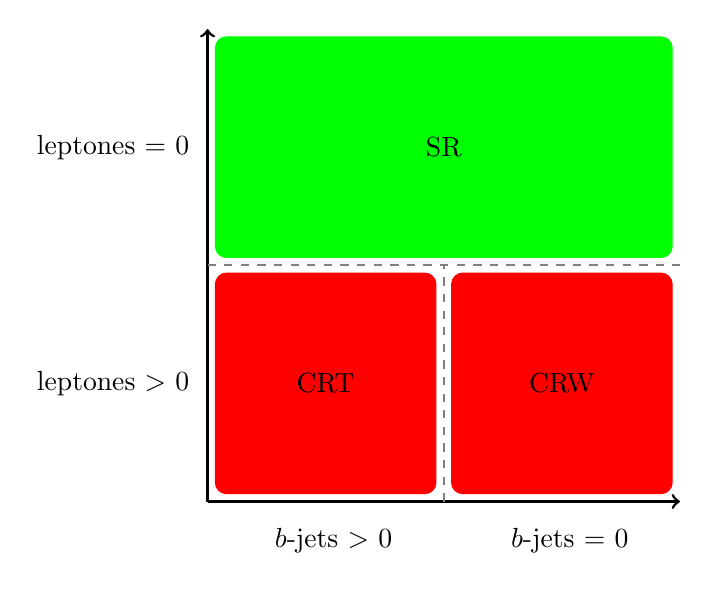
\begin{tikzpicture}[domain=0:4]

  \tikzstyle{region} = [rounded corners, fill]

  \draw[line width=1, ->] (0,0) -- (6,0);
  \draw[line width=1, ->] (0,0) -- (0,6);

  \draw[gray, dashed, line width=0.8] (0, 3.0) -- (6.0, 3.0);
  \draw[gray, dashed, line width=0.8] (3.0, 0) -- (3.0, 3.0);

  \draw node at (1.6,-0.5) {$b$-jets $>$ 0};
  \draw node at (4.6,-0.5) {$b$-jets = 0};
  \draw node at (-1.2, 1.5) {leptones $>$ 0};
  \draw node at (-1.2, 4.5) {leptones = 0};

  \draw[green, region] (0.1,3.1) rectangle (5.9,5.9);
  \draw node at (3.0,4.5) {SR};

  \draw[red, region] (0.1,0.1) rectangle (2.9,2.9) ;
  \draw node at (1.5,1.5) {CRT};

  \draw[red, region] (3.1,0.1) rectangle (5.9,2.9) ;
  \draw node at (4.5,1.5) {CRW};

\end{tikzpicture}
}

  \caption{Regiones de control definidas para normalizar el fondo de {\wgam} (CRW) y {\ttgam} (CRT). En este contexto 'leptón' se refiere solo a electrones o muones.}
  \label{fig:bkg_crt_crw}
\end{figure}



\begin{table}[!htbp]
  \centering

  \caption{Selección para las regiones de control utilizadas para normalizar los
    fondos de {\wgam}, {\ttgam} y {\gjet}, asociadas a las regiones de señal
    {\SRL} y {\SRH}}
  \label{tab:bkg_crs}

  \begin{tabularx}{\textwidth}{r|CCC|CCC}

    \hline
                                        & \multicolumn{3}{c|}{\SRL} & \multicolumn{3}{c}{\SRH} \\
    \cline{2-7}
                                       &      \CRWL &      \CRTL &   \CRQL &     \CRWH &    \CRTH  &   \CRQH  \\
  \hline
  $\pt^\gamma$ [\gev] $>$              &        125 &        125 &    125 &       150 &      150  &     300 \\
  $N_\mathrm{leptones}$                &          1 &    $\ge 1$ &      0 &         1 &  $\ge 1$  &       0 \\
  {\met} [\gev]                        &  [100-200] &   [80-200] &  $<50$ &  [100-200] & [80-200] &   $<50$ \\
  $N_\mathrm{jets} \ge$                &          4 &          4 &      4 &         2 &        2  &       2 \\
  $N_{b\text{-jets}}$                  &          0 &    $\ge 1$ &      - &         0 &  $\ge 1$  &       - \\
  $\pt^{j_1},\pt^{j_2}$ [\gev] $>$     &        100 &        100 &    100 &        40 &       40  &      40 \\
  $\dphijm >$                          &        0.4 &        0.4 &    0.4 &       0.4 &      0.4  &     0.4 \\
  $\rt <$                              &          - &          - &   0.85 &         - &        -  &       - \\
  {\HT} [\gev] $>$                     &          - &          - &      - &         - &        -  & $800$ \\
  $\dphijg <$                          &          - &          - &      - &       2.0 &      2.0  &     2.0 \\ % &    2.0 \\
  \hline
  \end{tabularx}

\end{table}


%% As seen in \Fig \ref{fig:sig_CR}, the signal contamination in the CRs is
%% expected to be small. For CRM, the low \MET cut kills most of the signal events,
%% keeping its fraction below 0.5\% across the whole grid and decreasing with the
%% gluon mass.

%% ## CRLW_2
%% Percentage of wgamma:  63.26 % 3.81429171562 / 6.02966526151
%% Largest contamination:  41.84 %
%% ## CRLW_3
%% Percentage of wgamma:  69.18 % 15.5461444855 / 22.4714100622
%% Largest contamination:  11.3 %
%% ## CRLT_2
%% Percentage of ttbarg:  55.83 % 8.56628704071 / 15.3442126885
%% Largest contamination:  74.96 %
%% ## CRLT_3
%% Percentage of ttbarg:  60.23 % 14.3853740692 / 23.8827633113
%% Largest contamination:  40.28 %

Es importante que las CR no tengan una contaminación de señal. Se aplica además
un corte superior en {\met} para reducir la contaminación de señal. En {\CRW} y
{\CRT} la contaminación de señal en las CR es $<3\%$ para la mayor parte de la
grid, aunque es mayor (hasta 70\%) para algunos puntos de baja masa de gluino en
{\CRTL} (ver \cref{fig:bkg_cr_contamination}). De cualquier forma, la
contaminación de señal se tiene en cuenta en el ajuste final para establecer los
limites de exclusión.


\begin{figure}[!htbp]
  \centering
  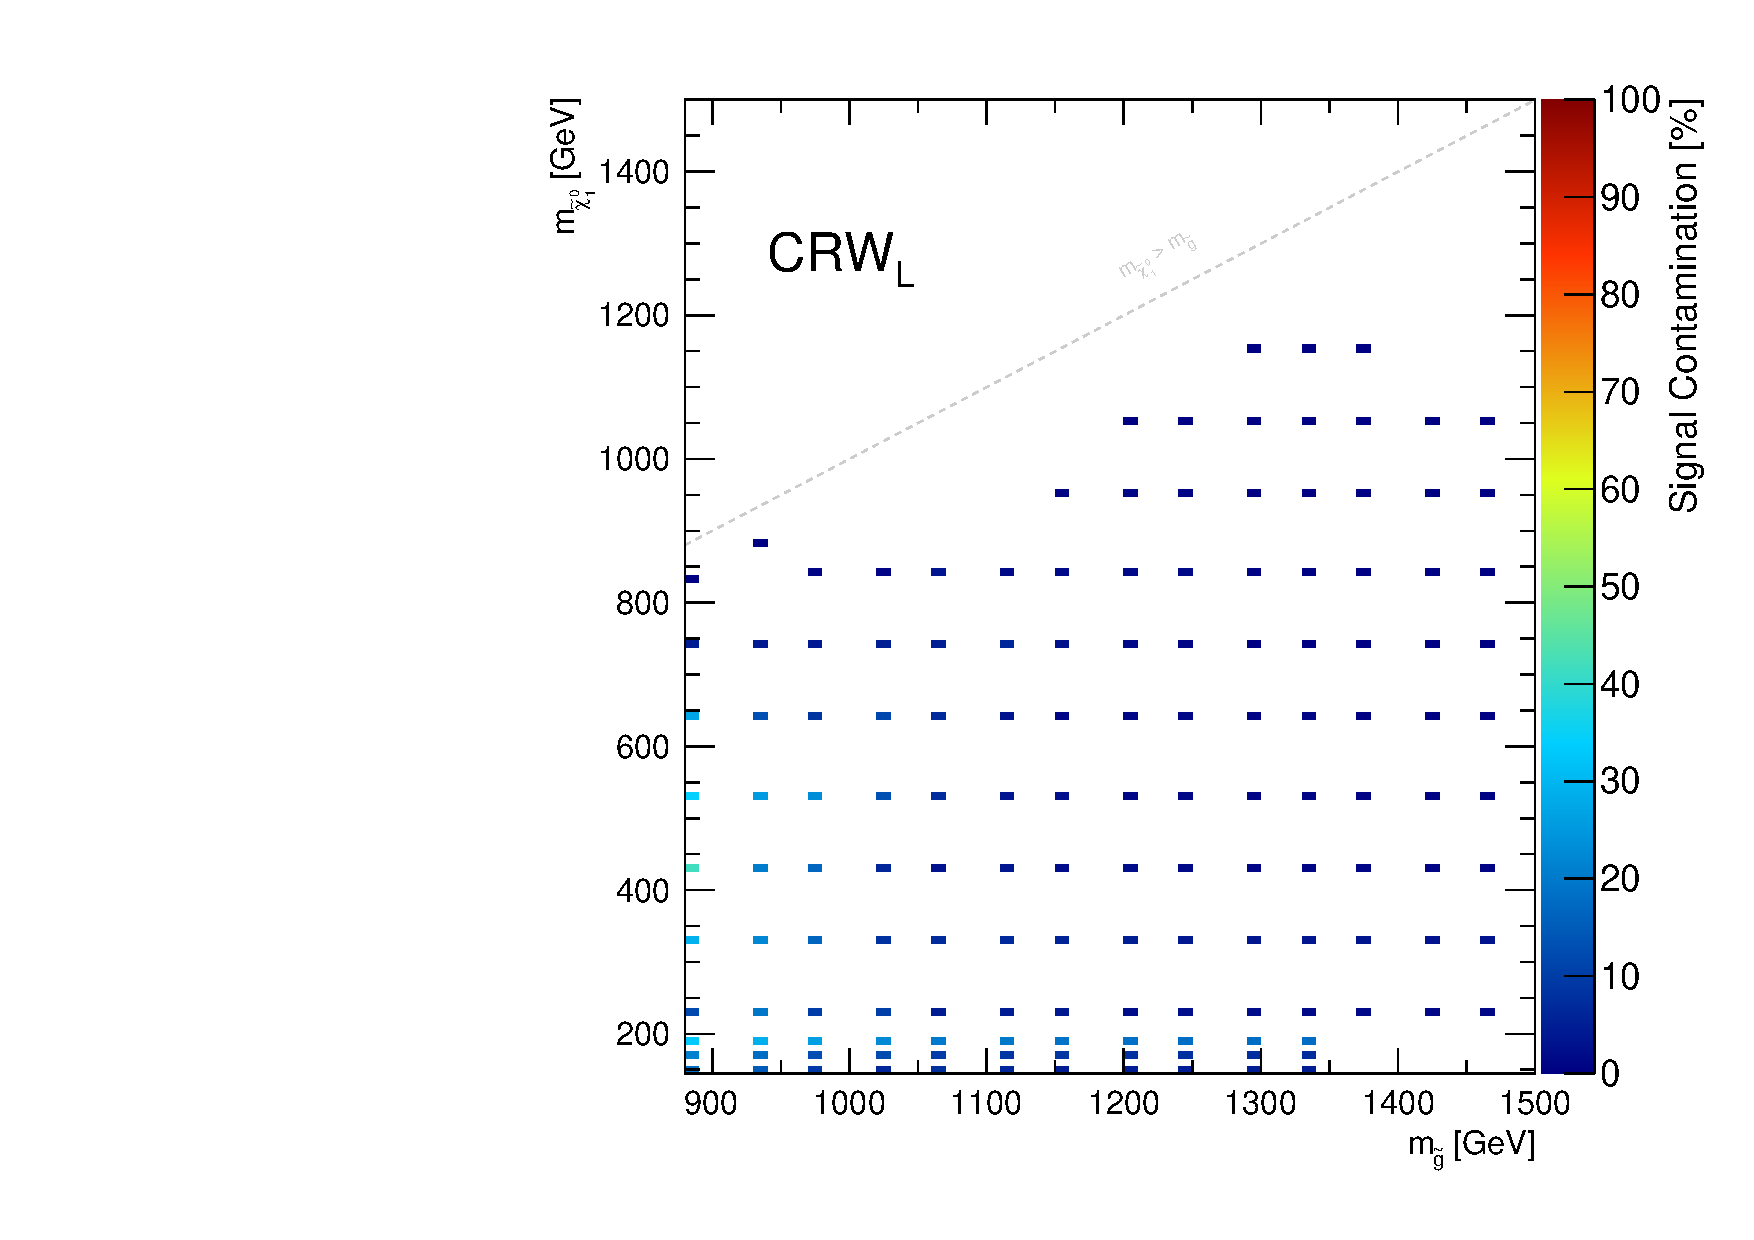
\includegraphics[width=0.49\textwidth]{figures/signal_contamination_crwl}
  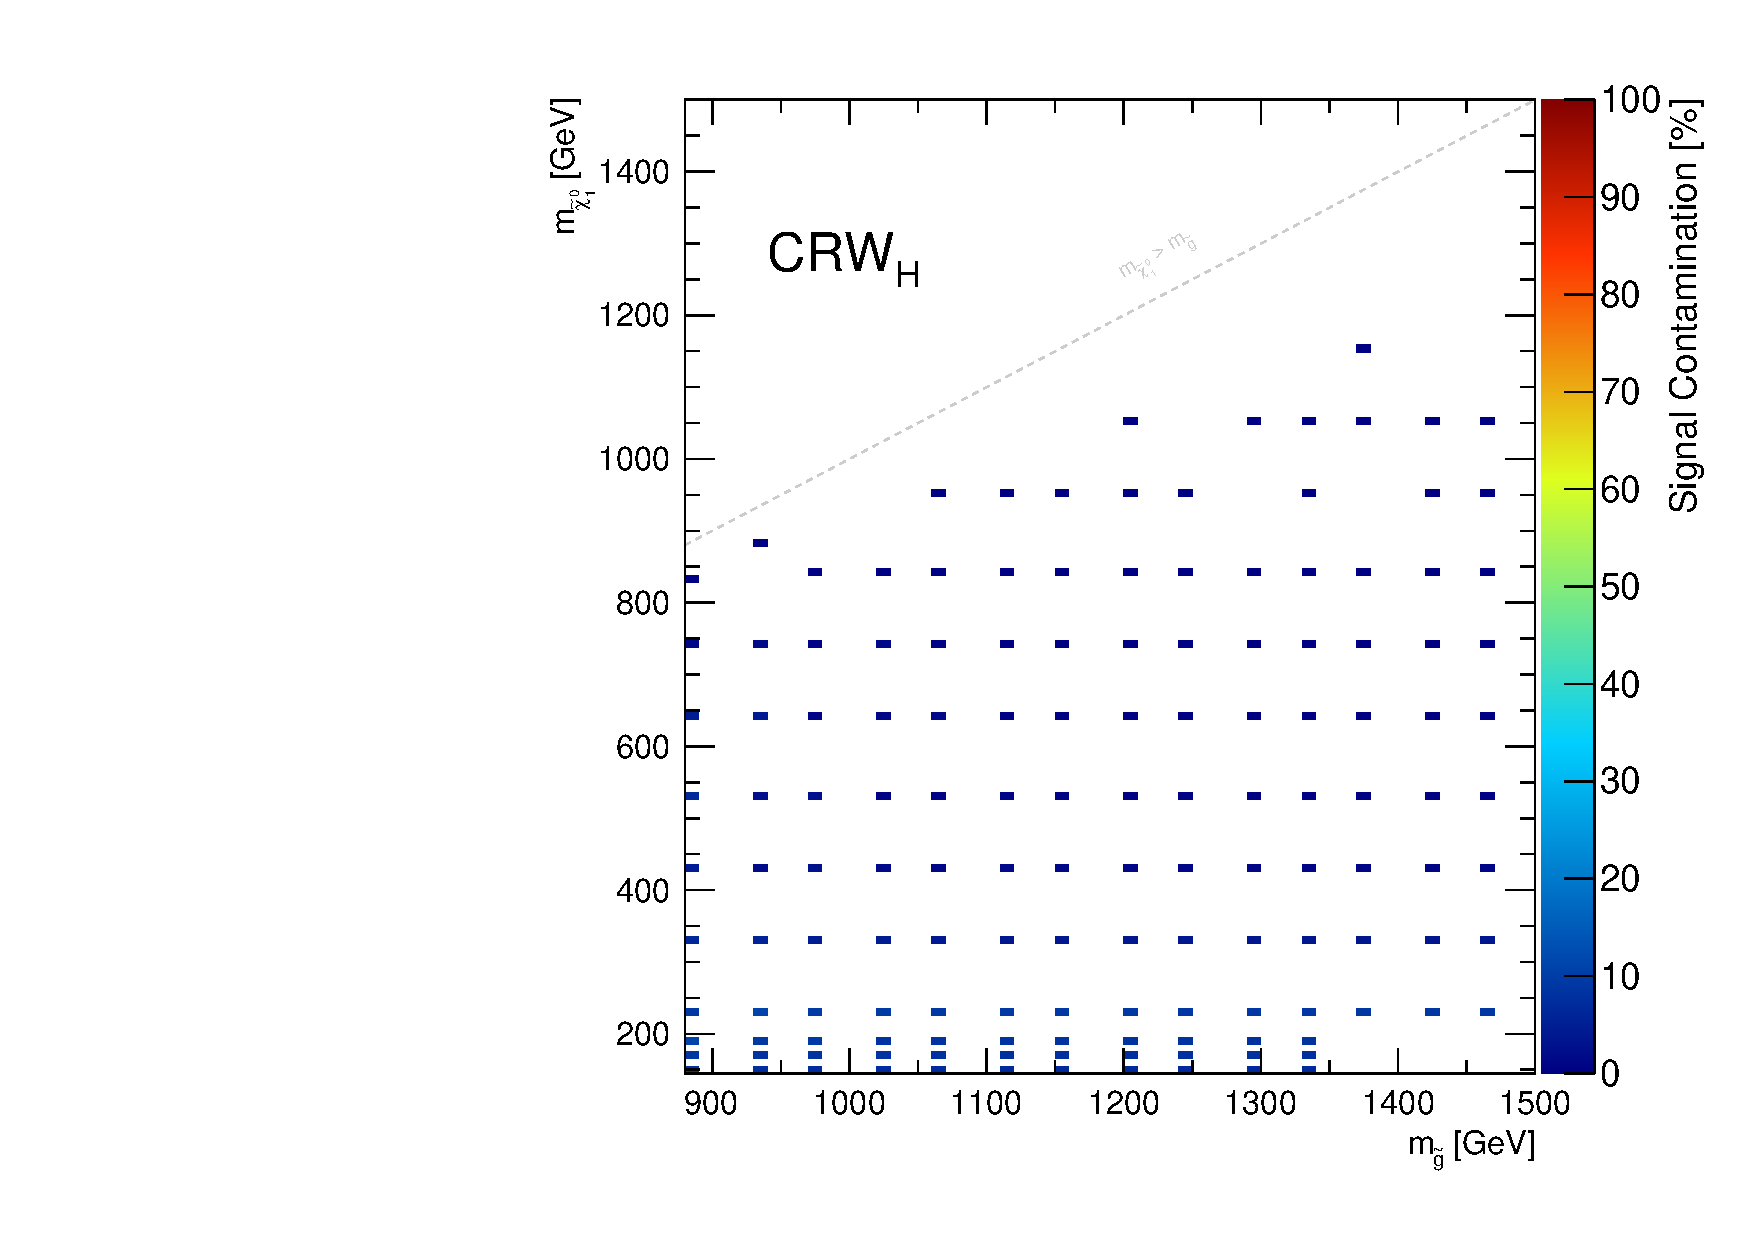
\includegraphics[width=0.49\textwidth]{figures/signal_contamination_crwh}

  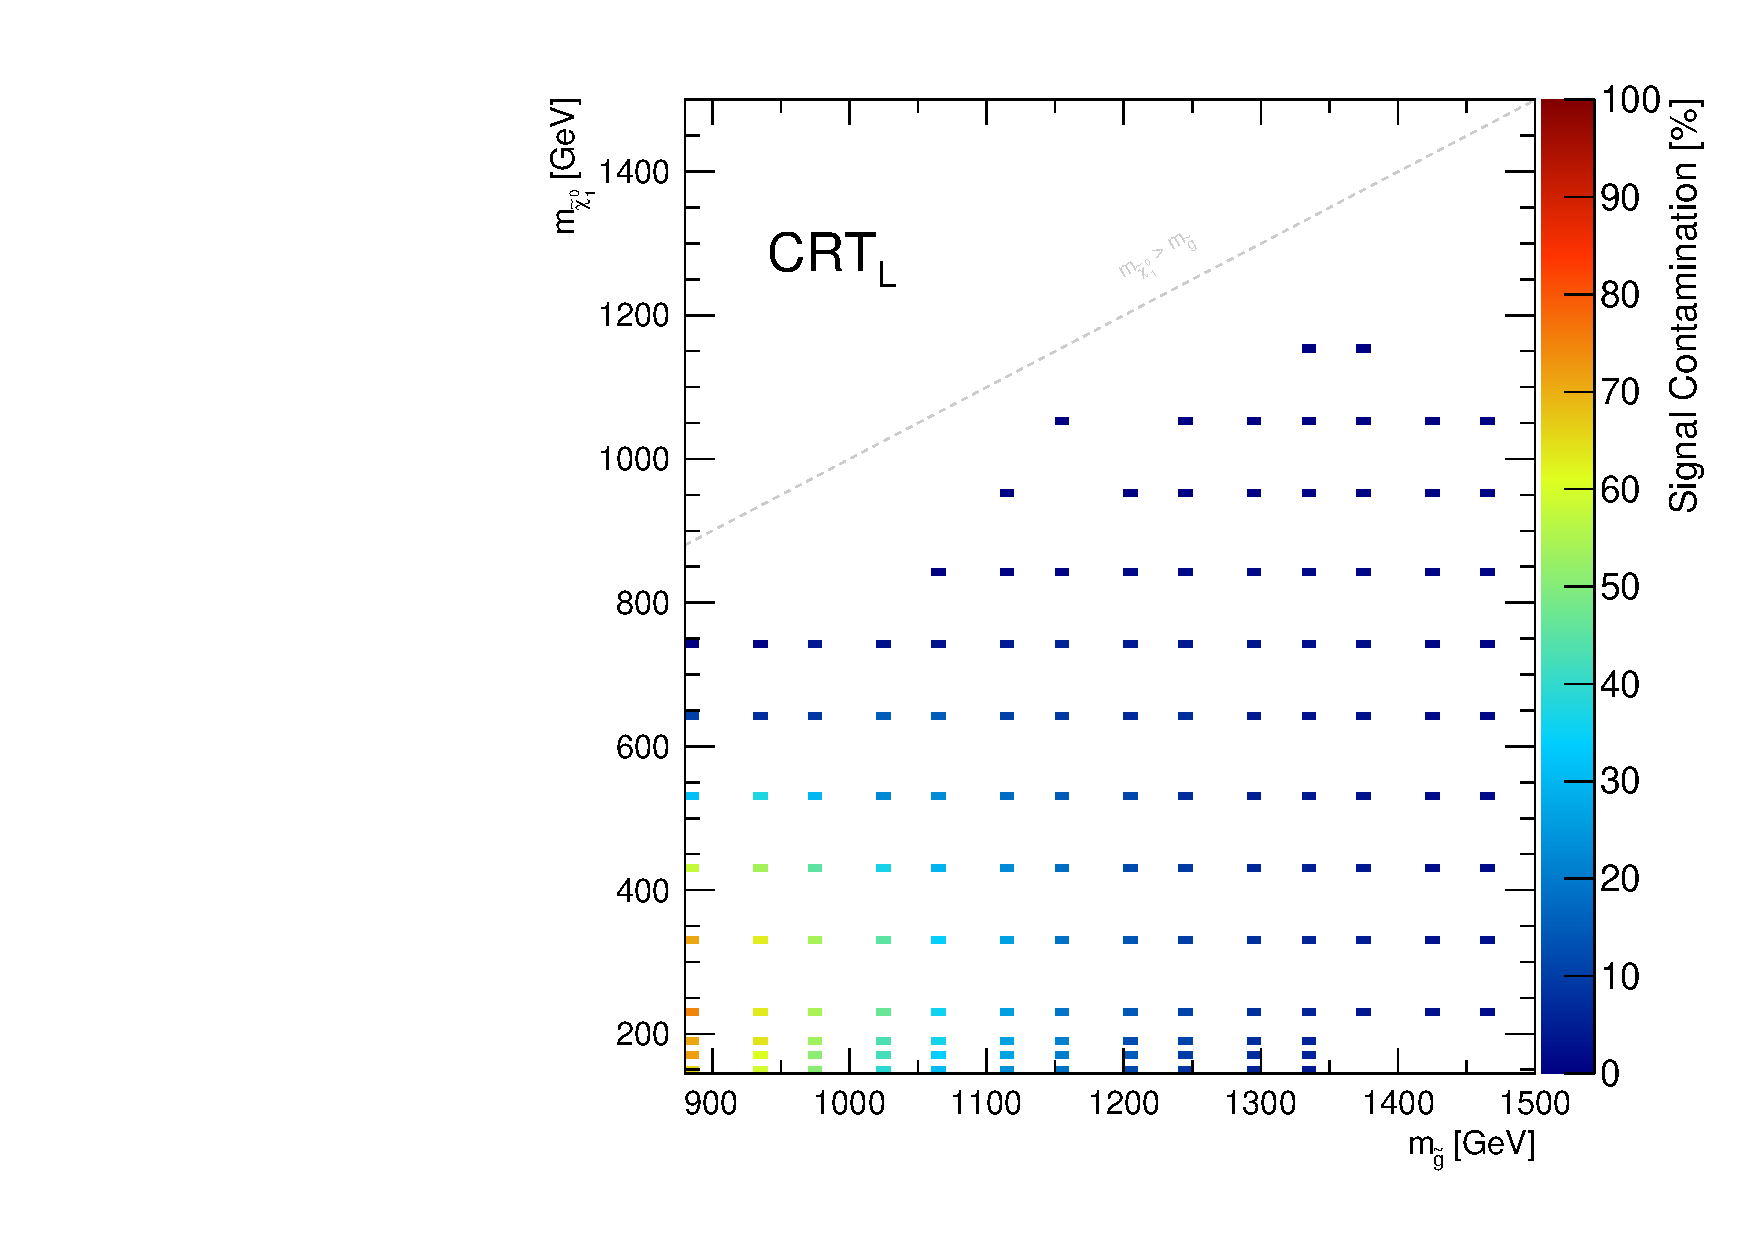
\includegraphics[width=0.49\textwidth]{figures/signal_contamination_crtl}
  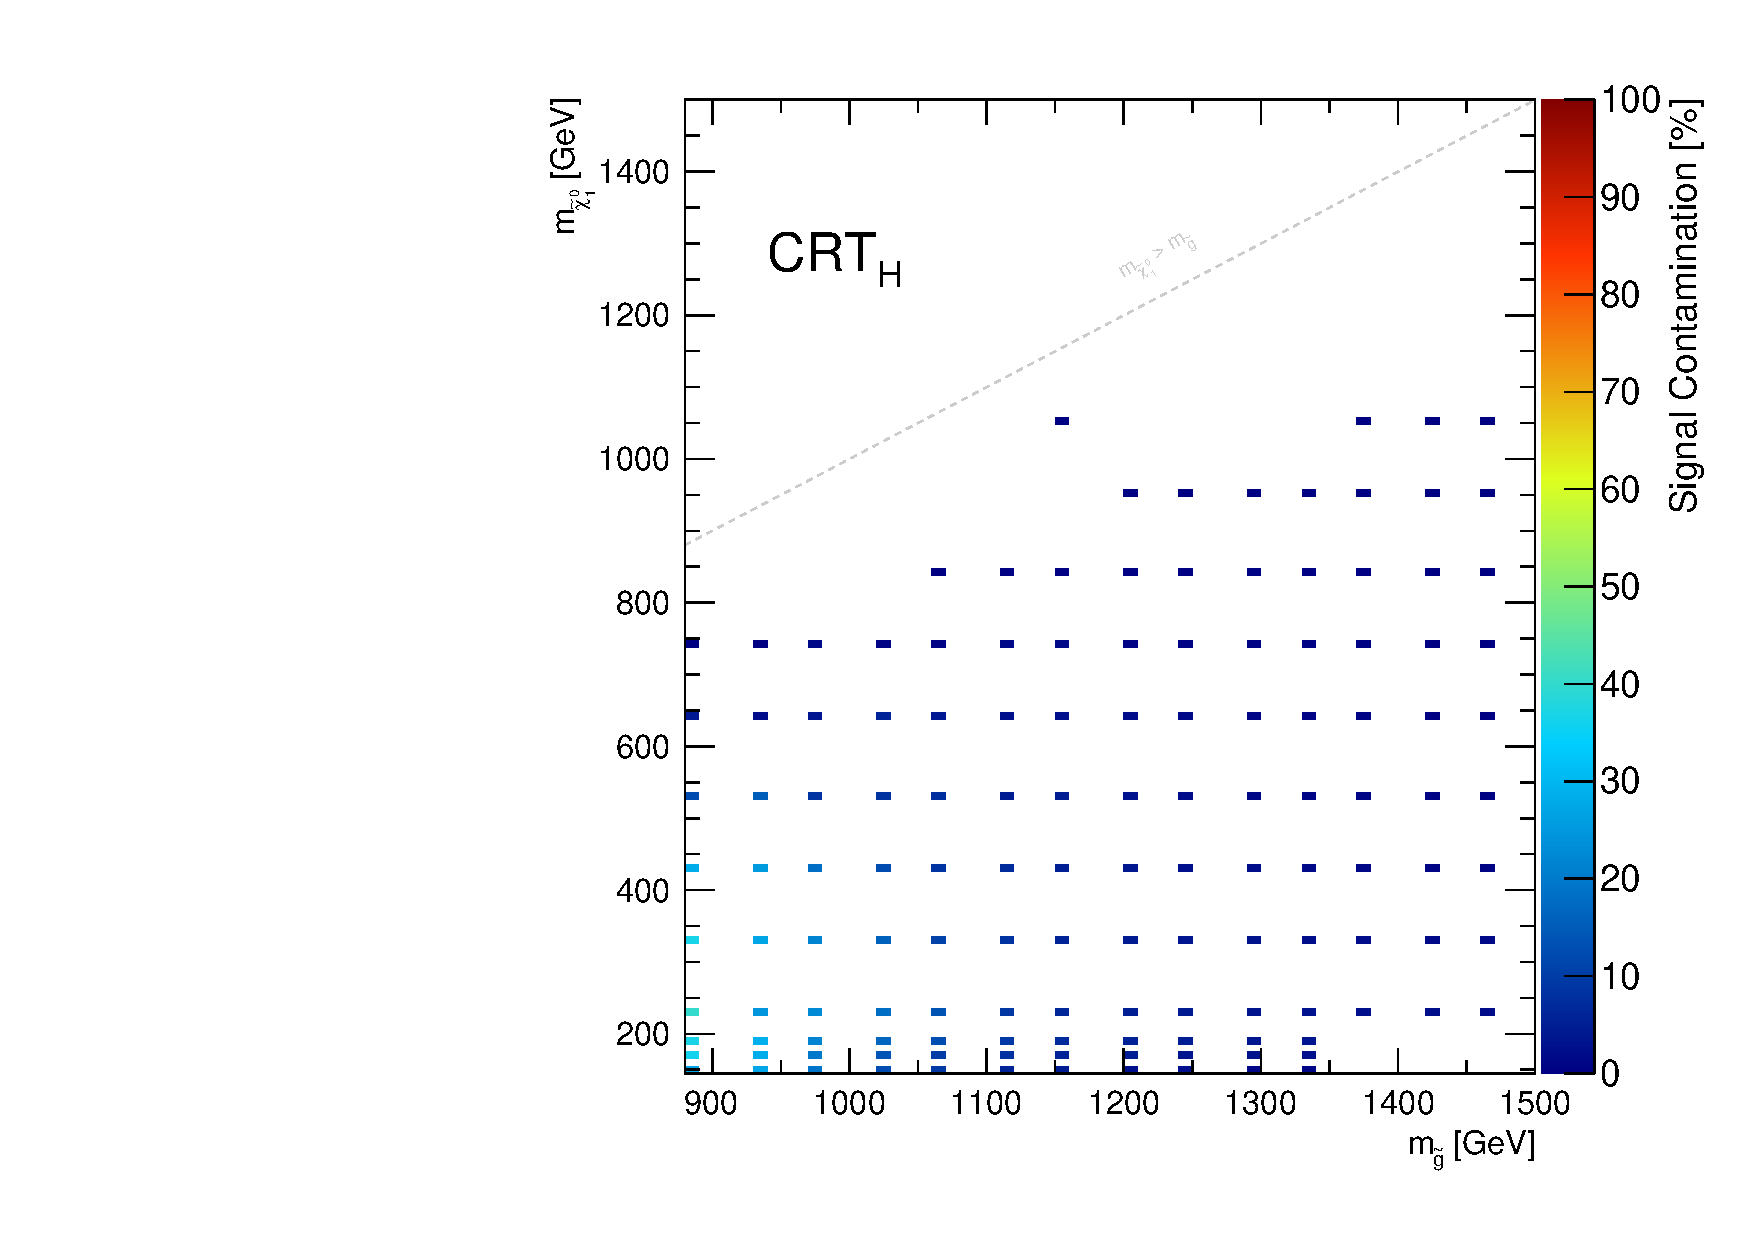
\includegraphics[width=0.49\textwidth]{figures/signal_contamination_crth}

  \caption{Contaminación de señal esperada en las regiones de control {\CRW} y {\CRT} asociadas a {\SRL} (izquierda) y {\SRH} (derecha).}
  \label{fig:bkg_cr_contamination}
\end{figure}



\subsection{Regiones de validación}

En la definición de las regiones de control, algunos cortes fueron relajados, o directamente removidos
respecto a las SR, para incrementar el número de eventos en las mismas. Para validar la extrapolación
entre las CR y la SR, se definen ciertas regiones de validación, imponiendo nuevamente los cortes de la SR, de
a uno a la vez.

De esta forma se definen las siguientes regiones de validación para {\CRW} y {\CRT}, donde la X se refiere a
la correspondiente CR (W o T). La seleccion detallada puede verse en \cref{tab:bkg_vrs1}.

\begin{description}
\item[\textbf{VRXM}] igual que CRX pero con el corte en {\met} como en la SR.
\item[\textbf{VRXR}]  igual que CRX pero con el corte en {\rt} como en la {\SRL} (solo para {\SRL}).
\item[\textbf{VRXH}]  igual que CRX pero con el corte en {\HT} como en la {\SRH} (solo para {\SRH}).
\end{description}

\begin{table}[!htbp]
  \centering

  \caption{Selección para las regiones de validación utilizadas para validar la extrapolación
    de los fondos de {\wgam}, {\ttgam}, entre las CR a las regiones de señal
    {\SRL} y {\SRH}}
  \label{tab:bkg_vrs1}

  \resizebox{\textwidth}{!}{
  \begin{tabular}{r|cccc|cccc}
    \hline
                                       & \multicolumn{4}{c|}{\SRL} & \multicolumn{4}{c}{\SRH} \\
    \cline{2-9}
                             &       VRWM &       VRWR &     VRTM &      VRTR &     VRWM &       VRWH &     VRTM &      VRTH \\
  \hline
  $\pt^\gamma$ [\gev] $>$    &        125 &        125 &      125 &      125  &      150 &        150 &      150 &      150  \\
  $N_\mathrm{leptones}$      &          1 &          1 &  $\ge 1$ &  $\ge 1$  &        1 &          1 &  $\ge 1$ &  $\ge 1$  \\
  {\met} [\gev]              &     $>200$ &  [100-200] &   $>200$ &  [80-200] &   $>300$ &  [100-200] &   $>300$ &  [80-200] \\
  $N_\mathrm{jets} \ge$      &          4 &          4 &        4 &         4 &        2 &          2 &        2 &         2 \\
  $N_{b\text{-jets}}$        &          0 &          0 &  $\ge 1$ &   $\ge 1$ &        0 &          0 &  $\ge 1$ &   $\ge 1$ \\
  $\pt^{j_1},\pt^{j_2}$ [\gev] $>$     &        100 &        100 &      100 &       100 &       40 &         40 &       40 &        40 \\
  $\dphijm >$                &        0.4 &        0.4 &      0.4 &       0.4 &      0.4 &        0.4 &      0.4 &       0.4 \\
  $\rt <$                    &          - &       0.85 &        - &      0.85 &        - &          - &        - &         - \\
  {\HT} [\gev] $>$           &          - &          - &        - &         - &        - &        800 &        - &       800 \\
  \hline
  \end{tabular}
  }

\end{table}



\section{Producción de fotones directos (\gjet)}
\label{sec:bkg_gjet}

Por diseño, la probabilidad de que eventos {\gjet} pasen a la región de señal es
baja, ya que resulta raro que estos eventos tengan una gran cantidad de {\met}.
A pesar de eso, esta energia faltante puede ser producida por la mal
reconstrucción de la energía de los jets. Y debido a que la sección eficaz de
estos procesos es muy alta, puede resulta en una contaminación significativa.

Para determinar este fondo no es posible confiar plenamente en las simulaciones MC.
Debido a la baja cantidad de eventos similares a la señal, solo eventos
muy raros de la simulacion son utiles y seria necesario una muestra MC con
una muy alta cantidad de eventos.

Por estos motivos se diseño una región de control en donde dominan los eventos de
{\gjet} a la que se llamo {\CRQ}. Los detalles de la selección se pueden ver en
la \cref{tab:bkg_crs}. Básicamente es la misma selección que la SR pero a bajo
{\met} ($\met < 50 \gev$), donde domina esta fondo. La contaminación de multijets
es independientemente estimada a partir de los datos como se explica en
\cref{sec:jetfakes}.

%% La estimación final del fondo de fotones directos es obtenida entonces normalizando los
%% eventos de la muestra MC en esta region de control.
%% The final estimate for the prompt photon background is obtained by normalizing the Sherpa MC events passing a dedicated selection (CRM) defined
%% from the corresponding SR but at low {\met} ($< 50 \gev$). As expected,  CRM selects an enriched sample %of events with similar kinematics to the SR but enriched in
%% of QCD background events. The multijet contamination is independently estimated with the ratio method explained in sec \ref{sec:jetfakes}. %, is explicitly removed from the selected sample to avoid double counting in the global fit described in sec \ref{sec:fitconfig}
%% Some intermediate {\met} regions between 50 {\gev} and the SR cut are kept for validation purposes. Given the large jet multiplicty and \MET requirements in SR2 and SR3, respectively, the prompt photon background is
%% expected to be very small in both signal regions. However, its contribution is not negligible in the control and validation regions so it is important to get a good normalization estimate.

%% ## CRM_2
%% Percentage of photonjet_sherpa:  87.65 % 1224.78869629 / 1397.31749731
%% Largest contamination:  0.67 %

%% ## CRM_3
%% Percentage of photonjet_sherpa:  87.54 % 156.909103394 / 179.23669574
%% Largest contamination:  0.35 %

La contaminación de señal en esta región de control es despreciable, debido a
que la señal posee gran cantidad de energía faltante, como puede verse en la
\cref{fig:bkg_cr_contamination}.

\begin{figure}[!htbp]
  \centering
  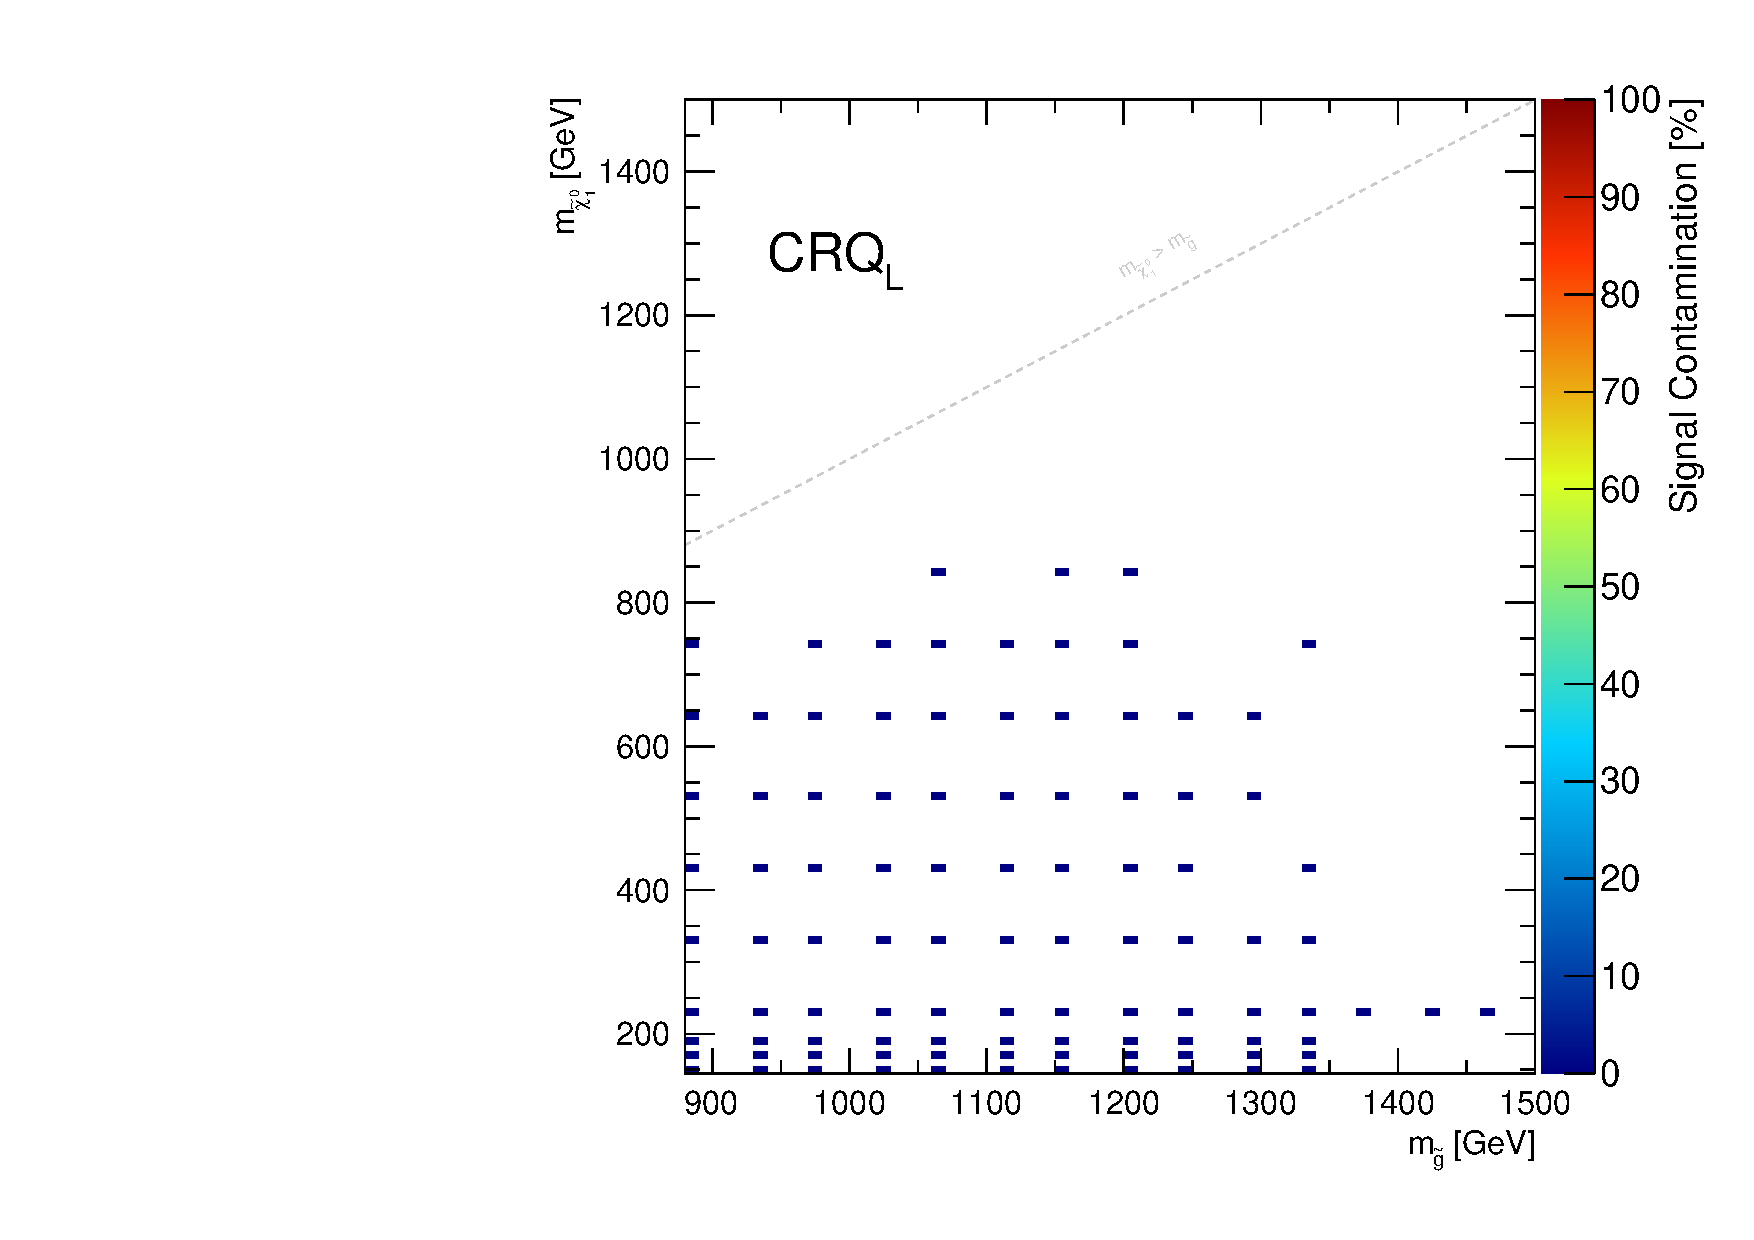
\includegraphics[width=0.49\textwidth]{signal_contamination_crql}
  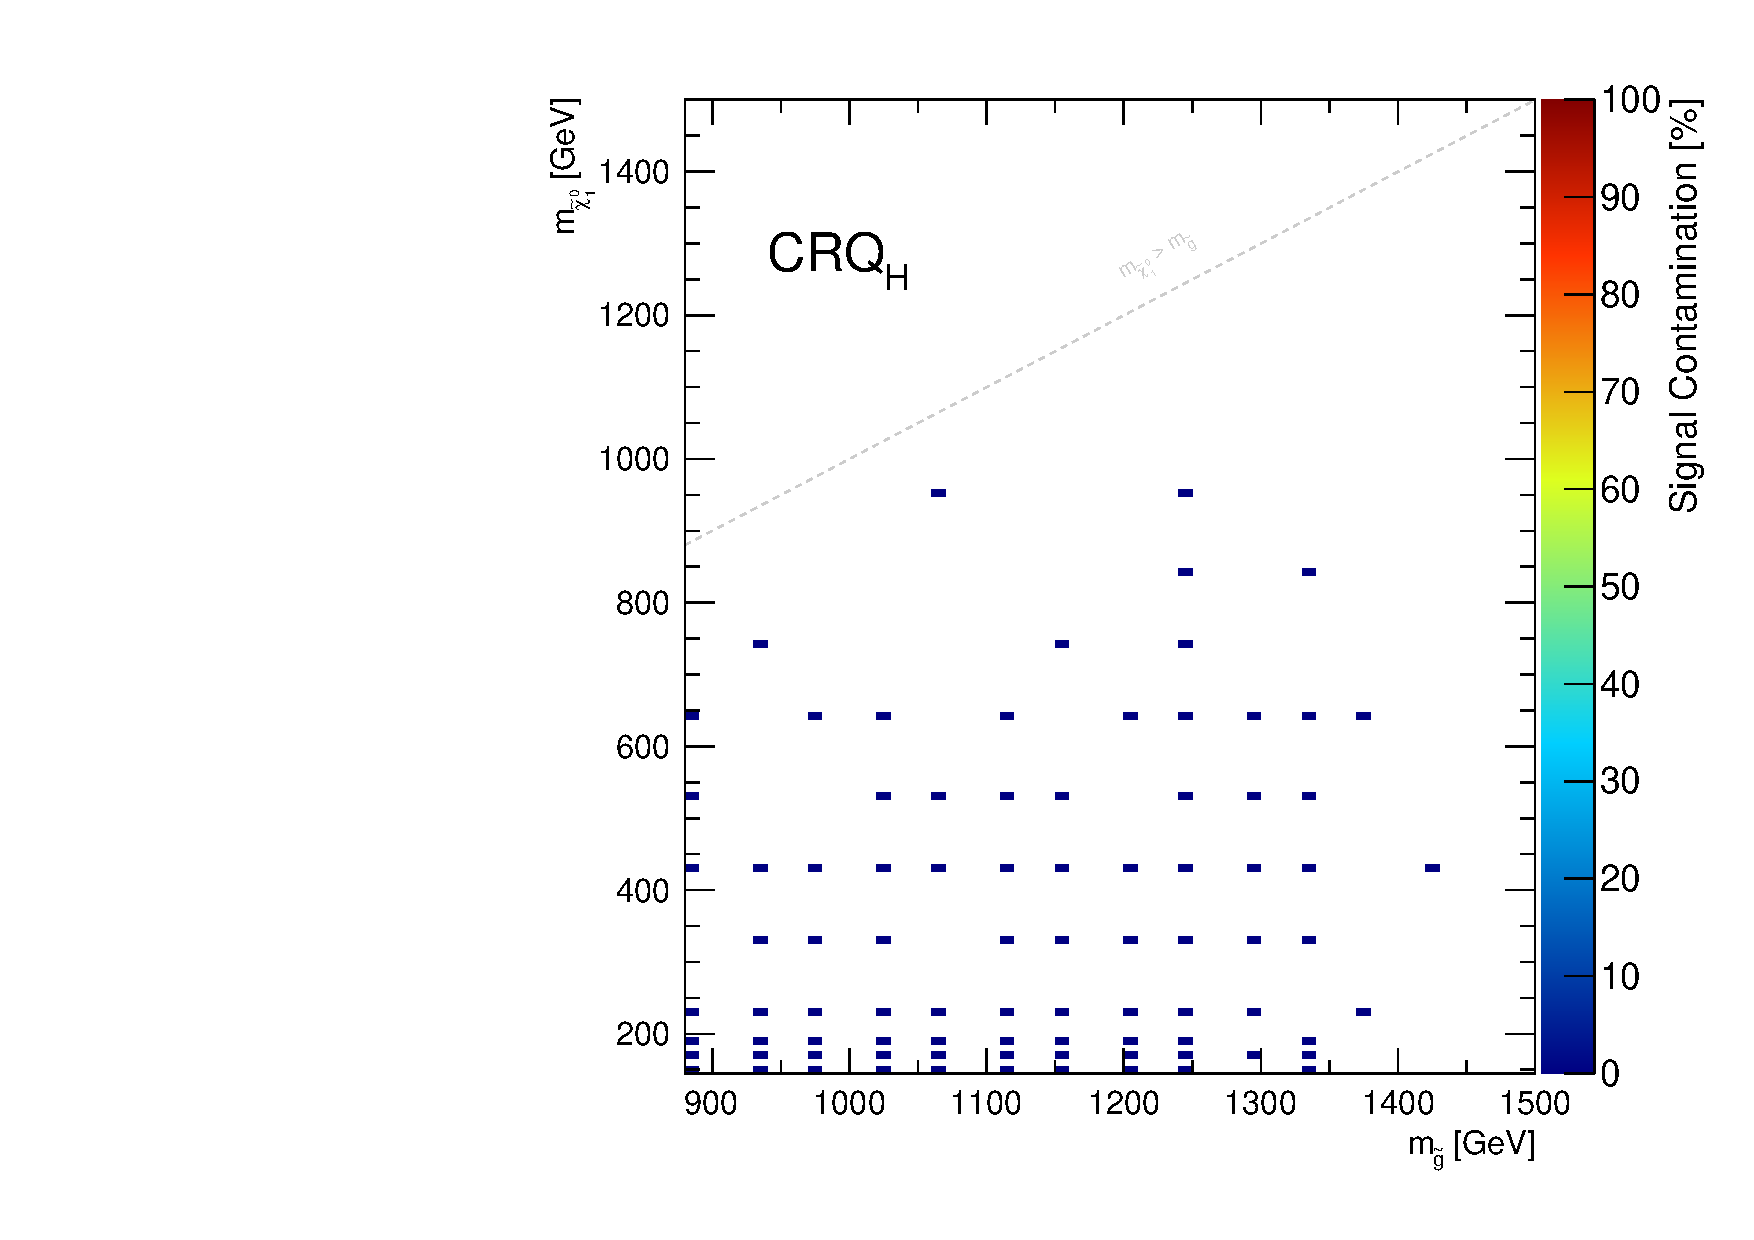
\includegraphics[width=0.49\textwidth]{signal_contamination_crqh}

  \caption{Contaminación de señal esperada en la región de control {\CRQ} asociada a {\SRL} (izquierda) y {\SRH} (derecha).}
  \label{fig:bkg_cr_contamination}
\end{figure}




\subsection{Comparación de generadores}

Acá comparación entre Pythia y Sherpa


\subsection{Regiones de validación}\label{sec:bkg_vrs2}

Se definen un conjunto de selecciones para validar los resultados de la
extrapolación de {\gjet} de la región de control a bajo {\met} hasta
las SR a alto {\met}. Las regiones de validación se definen lo más cerca posible
de las SR en el espacio de observables, revirtiendo algunos cortes para
hacerlas ortogonales a las SR, como se describe a continuación.

\begin{description}\itemsep0.1cm
\item[{\bf VRMX}] igual a la SR pero con un requerimiento intermedio en {\met}
  ($X\gev < \met < 150\gev$) con $X = 50,75,100$. El corte superior asegura la
  ortogonalidad con la SR.
\item[{\bf VRH}] igual a la SR pero invirtiendo el corte en {\HT} ($\HT<
  800\gev$). Solo definida para {\SRH}, ya que no hay un corte en {\HT} en
  {\SRL}.
\item[{\bf VRQ}] igual a la SR pero con el corte en {\dphijm} invertido ($
  \dphijm < 0.4$) para aumentar la contribución de fondos con {\met}
  instrumental.
\end{description}

En la figura \cref{fig:bkg_crq} pueden verse los esquemas de la definición de las CR y VR.

\begin{figure}[!htbp]
  \centering

  \resizebox{0.49\textwidth}{!}{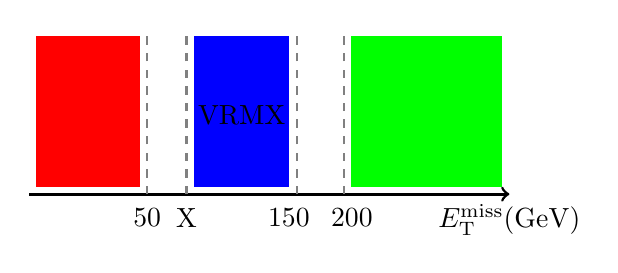
\begin{tikzpicture}[domain=0:4]

  \tikzstyle{region} = [fill]

  \draw[line width=1, ->] (0,0) -- (6.1,0) node[below] {$E_\mathrm{T}^\mathrm{miss} (\mathrm{GeV})$};
  %% \draw[line width=1, ->] (0,0) -- (0,3.1);

  \draw[gray, dashed, line width=0.8] (1.5, 0) -- (1.5, 2.1);
  \draw[gray, dashed, line width=0.8] (4.0, 0) -- (4.0, 2.1);
  \draw[gray, dashed, line width=0.8] (2.0, 0) -- (2.0, 2.1);
  \draw[gray, dashed, line width=0.8] (3.4, 0) -- (3.4, 2.1);

  \draw node at (1.5,-0.3) {50};
  \draw node at (2.0,-0.3) {X};
  \draw node at (3.3,-0.3) {150};
  \draw node at (4.1,-0.3) {200};

  \draw[green, region] (4.1,0.1) rectangle (6,2);
  \draw node at (5.0,1) {\SRL};

  \draw[red, region] (0.1,0.1) rectangle (1.4,2) ;
  \draw node at (0.75, 1) {\CRQ};

  \draw[blue, region] (2.1,0.1) rectangle (3.3,2) ;
  \draw node at (2.7,1) {VRMX};


\end{tikzpicture}
}
  \resizebox{0.49\textwidth}{!}{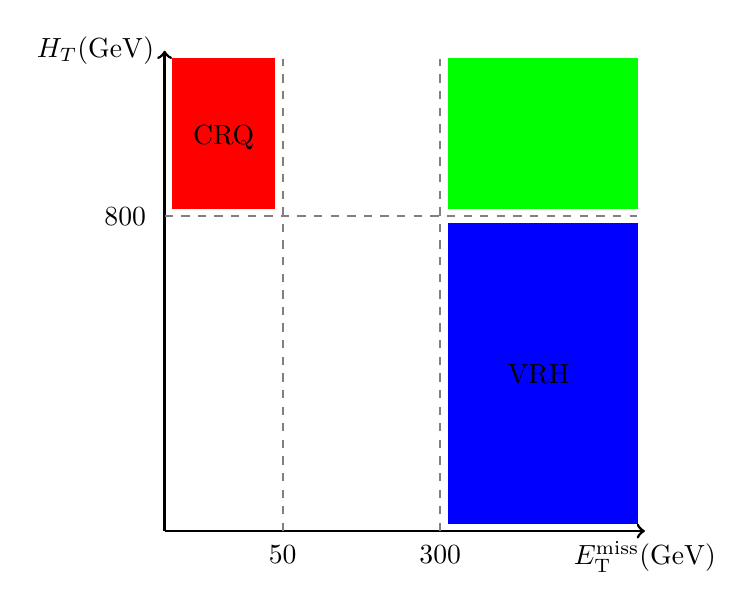
\begin{tikzpicture}[domain=0:4]

  \tikzstyle{region} = [fill]


  \draw[line width=1, ->] (0,0) -- (0,6.1) node[left] {$H_T (\mathrm{GeV})$};
  \draw[line width=1, ->] (0,0) -- (6.1,0) node[below] {$E_\mathrm{T}^\mathrm{miss} (\mathrm{GeV})$};

  %% \draw[gray, dashed, line width=0.8] (0, 2.5) -- (6, 2.5);
  \draw[gray, dashed, line width=0.8] (0, 4.0) -- (6, 4.0) node[black] at (-0.5,4.0) {800};
  \draw[gray, dashed, line width=0.8] (1.5, 0) -- (1.5, 6) node[black] at (1.5,-0.3) {50};
  \draw[gray, dashed, line width=0.8] (3.5, 0) -- (3.5, 6) node[black] at (3.5,-0.3) {300};

  \draw[green, region] (3.6,4.1) rectangle (6,6);
  \draw node at (4.75,5.0) {\large \SRH};

  \draw[red, region] (0.1,4.1) rectangle (1.4,6) ;
  \draw node at (0.75, 5) {CRQ};

  \draw[blue, region] (3.6,0.1) rectangle (6,3.9) ;
  \draw node at (4.75,2.) {VRH};

\end{tikzpicture}
}

  \caption{Esquema de las regiones de control diseñadas para normalizar el fondo
    de {\gjet} para {\SRL} (izquierda) y {\SRH} (derecha). También se muestran
    las regiones de validación utilizadas para validar la extrapolación
    $\mathrm{CR}\to\mathrm{SR}$.}
  \label{fig:bkg_crq}
\end{figure}



%----------------
% Electron fakes
%----------------
\section{Electrones identificados como fotones} \label{sec:efakes}

Los eventos en los que un electrón de alto {\pt} sea identificado como un \note{Bocci:1643300}
fotón, pueden contaminar alguna de las SR. Esta contaminación
proviene generalmente de procesos del SM como $W(\to e\nu)$+ jets, $Z(\to ee)$ +
jets y {\ttbar}.

Como se mencionó en \cref{sec:obj_photons}, los electrones y fotones dejan
lluvias electromagnéticas muy similares en el detector. Los algoritmos de
reconstrucción de fotones están diseñados para reducir la identificación erronea
de electrones como fotones, aunque sin embargo, para poder mantener una alta
eficiencia de reconstrucción, no se realiza un distinción demasiado estricta. En
caso de duda, los clusters electromagnéticos, son reconstruidos bajo ambas
hipótesis (electrón o fotón) y guardados (duplicados) en ambas categorias. Esto
implica que electrones pueden terminar siendo reconstruidos como fotones, y si este
pasa la selección de fotones utilizada en el
análisis, contribuira al fondo por mala identificación $e\to\gamma$.


Los electrones son reconstruidos de los clusters asociados a una traza, mientras
que los fotones son reconstruidos de los clusters que no tienen ninguna traza
asociada (candidatos a fotones no-convertidos) o asociado a un vértice de
conversión (candidatos a fotones convertidos). Se consideran los vértices con
una o dos trazas en la reconstrucción de fotones convertidos, y por lo tanto los
fotones convertidos pueden ser categorizados como fotones convertidos con una
traza o dos trazas. La traza de los candidatos a fotón convertidos con una sola
traza debe poseer un impacto en la B-layer. Se espera que una fracción de
electrones pueda ser reconstruida como fotones convertidos, por ejemplo, si
falla la asociación de la traza a un impacto en la B-layer, o si se asocia un
vértice de conversión espurio a ella. También si falla el algoritmo que asocia
la traza al cluster el electrón puede ser reconstruido como un fotón
no-convertido.

La fracción de electrones reconstruidos como fotones, depende claramente del
material en el detector, es por eso que pueden existir diferencias si se calcula
a partir de simulaciones Monte Carlo, ya que el material en las simulaciones no
es perfecto. Por tal motivo se calcula a partir de los datos, aunque también se
realiza una comparación con las muestras MC.

La estimación del fondo en la SR se calcula como,

\begin{equation}
  N_{e\to\gam}^{\mathrm{SR}} = \feg \cdot N_e^{\mathrm{SR}}
\end{equation}
%
donde $N_e^{\mathrm{SR}}$ es el número de eventos en la muestra de electrones
obtenida invirtiendo el rol de fotones y electrones en la selección de la región
de señal, es decir, se requiere un electrón aislado de alto {\pt}, y los fotones de señal son
vetados. Y {\feg} es la probabilidad de que electrón sea identificado
erróneamente como un fotón.


Para estimar la probabilidad de identificar erróneamente un electrón como un
fotón {\feg} se utiliza un método llamado \emph{tag and probe}, en una muestra
de eventos de datos {\Zee} que pasan el mismo trigger de fotones que utiliza el
análisis y la misma preselección (ver \cref{sec:event_baseline}). Adicionalmente, se
aplica un corte de $\met < 40 \gev$ para reducir la posible contaminación de
fotones reales de eventos de {\wgam}.

El método consiste en seleccionar un electrón (el electrón \emph{tag}) que
pasa un criterio de identificación \emph{tight} y que tener $20
\gev < \pt < 125 \gev$. Luego se busca un segundo candidato a electrón o fotón
(el objeto \emph{probe}). Este puede ser un electrón \emph{tight} o un fotón
\emph{tight}, ambos con $\pt > 125\gev$ y satisfaciendo los requerimientos de
aislamiento correspondientes.

Los valores de la masa de los pares de objetos seleccionados son guardados
separadamente para los tres casos posibles: dos electrones, un electrón y un
fotón convertido, o un electrón y fotón no-convertido. En los tres casos se
puede ver un pico alrededor del valor de la masa del bosón $Z$ ($\sim 91
\gev$).
Como el bosón $Z$ no puede decaer directamente en un electrón y un fotón, los
pares electrón-fotón que aparecen bajo el pico del $Z$ corresponden a electrones
mal identificados. Sin embargo, lo mismo aplica a otras partículas que decaen en
pares de electrones y por lo tanto es necesario utilizar algún método de
sustracción del fondo. Este deberá también tener en cuenta la contaminación por
las combinaciones aleatorias.

La probabilidad de identificación errónea {\feg} puede estimarse entonces como:

\begin{equation}\label{eq:efakerate}
  \feg = \frac{N_{e\gam}}{N_{ee}}
\end{equation}
%
donde $N_{e\gam}$ ($N_{ee}$) es el número de pares electrón-fotón
(electrón-electrón) encontrados en una ventana alrededor del pico del bosón $Z$ en la distribución de
la masa invariante, definida en el rango $81 < m_{ex} < 101 \gev$. Para obtener
el número de eventos $N_{ex}$, se realiza un ajuste de la distribución de la
masa invariante para los dos tipos de eventos utilizando un modelo de
señal+fondo. Este procedimiento se lleva a cabo de forma separada para fotones
convertidos y no-convertidos, y en clases del {\abseta} de los objetos
\emph{probe}. El bajo número de eventos disponibles hace imposible utilizar
clases de {\pt}, aunque de esta forma la estimación es conservativa ya que la
probabilidad de identificación errónea decrece con el {\pt} del electrón
\cite{Kuhl:1604846}.

Como modelo de señal se utiliza la suma de función \emph{Crystall-Ball} y una
Gausiana, mientras que para el modelo de fondo se utiliza un polinomio de grado
dos. En la \cref{fig:invmass_pairs} se puede ver las distribuciones de la masa
invariante para pares de $ee$ y $e\gam$, para la selección inclusiva, y los
correspondientes ajustes del modelo.

\begin{figure}[!htbp]
  \centering

  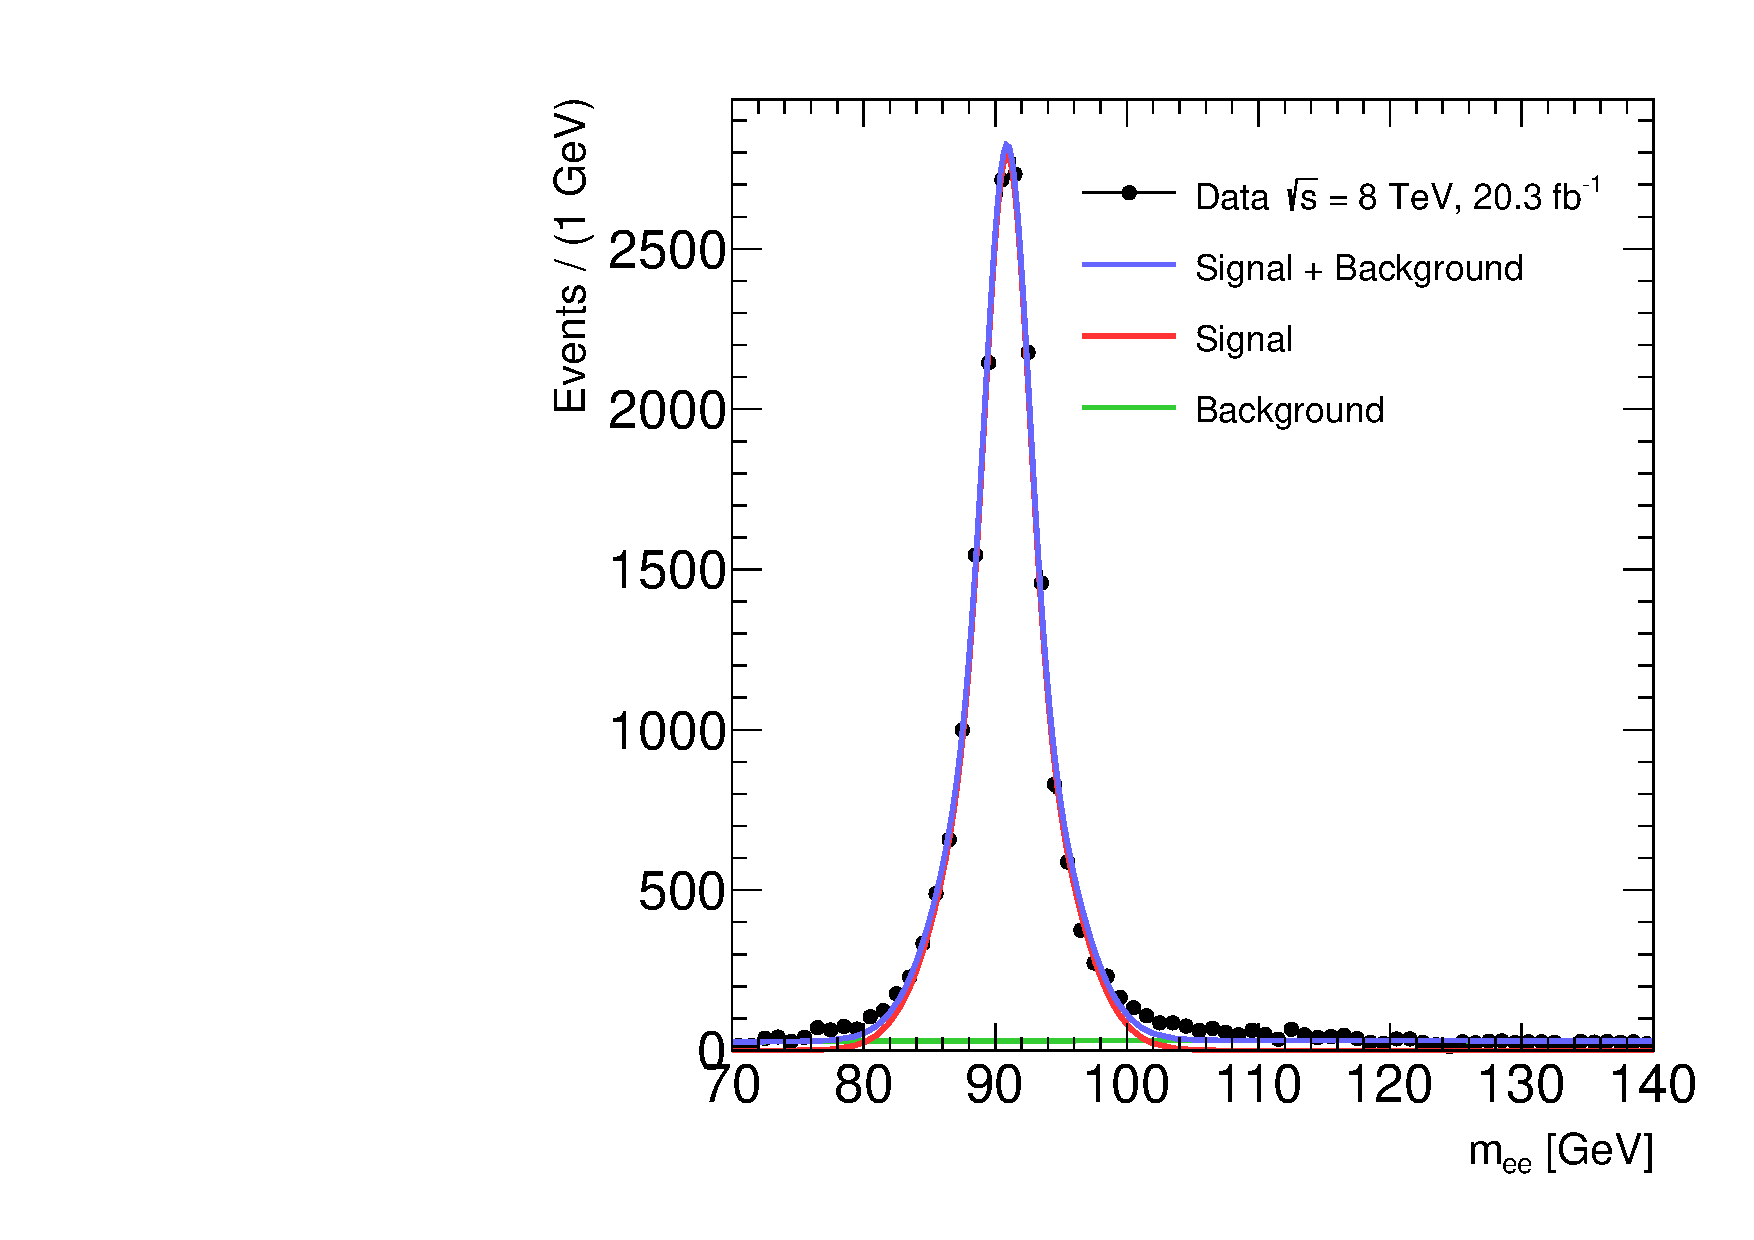
\includegraphics[width=0.49\textwidth]{figures/Fit_mee_efakes_Data_all}
  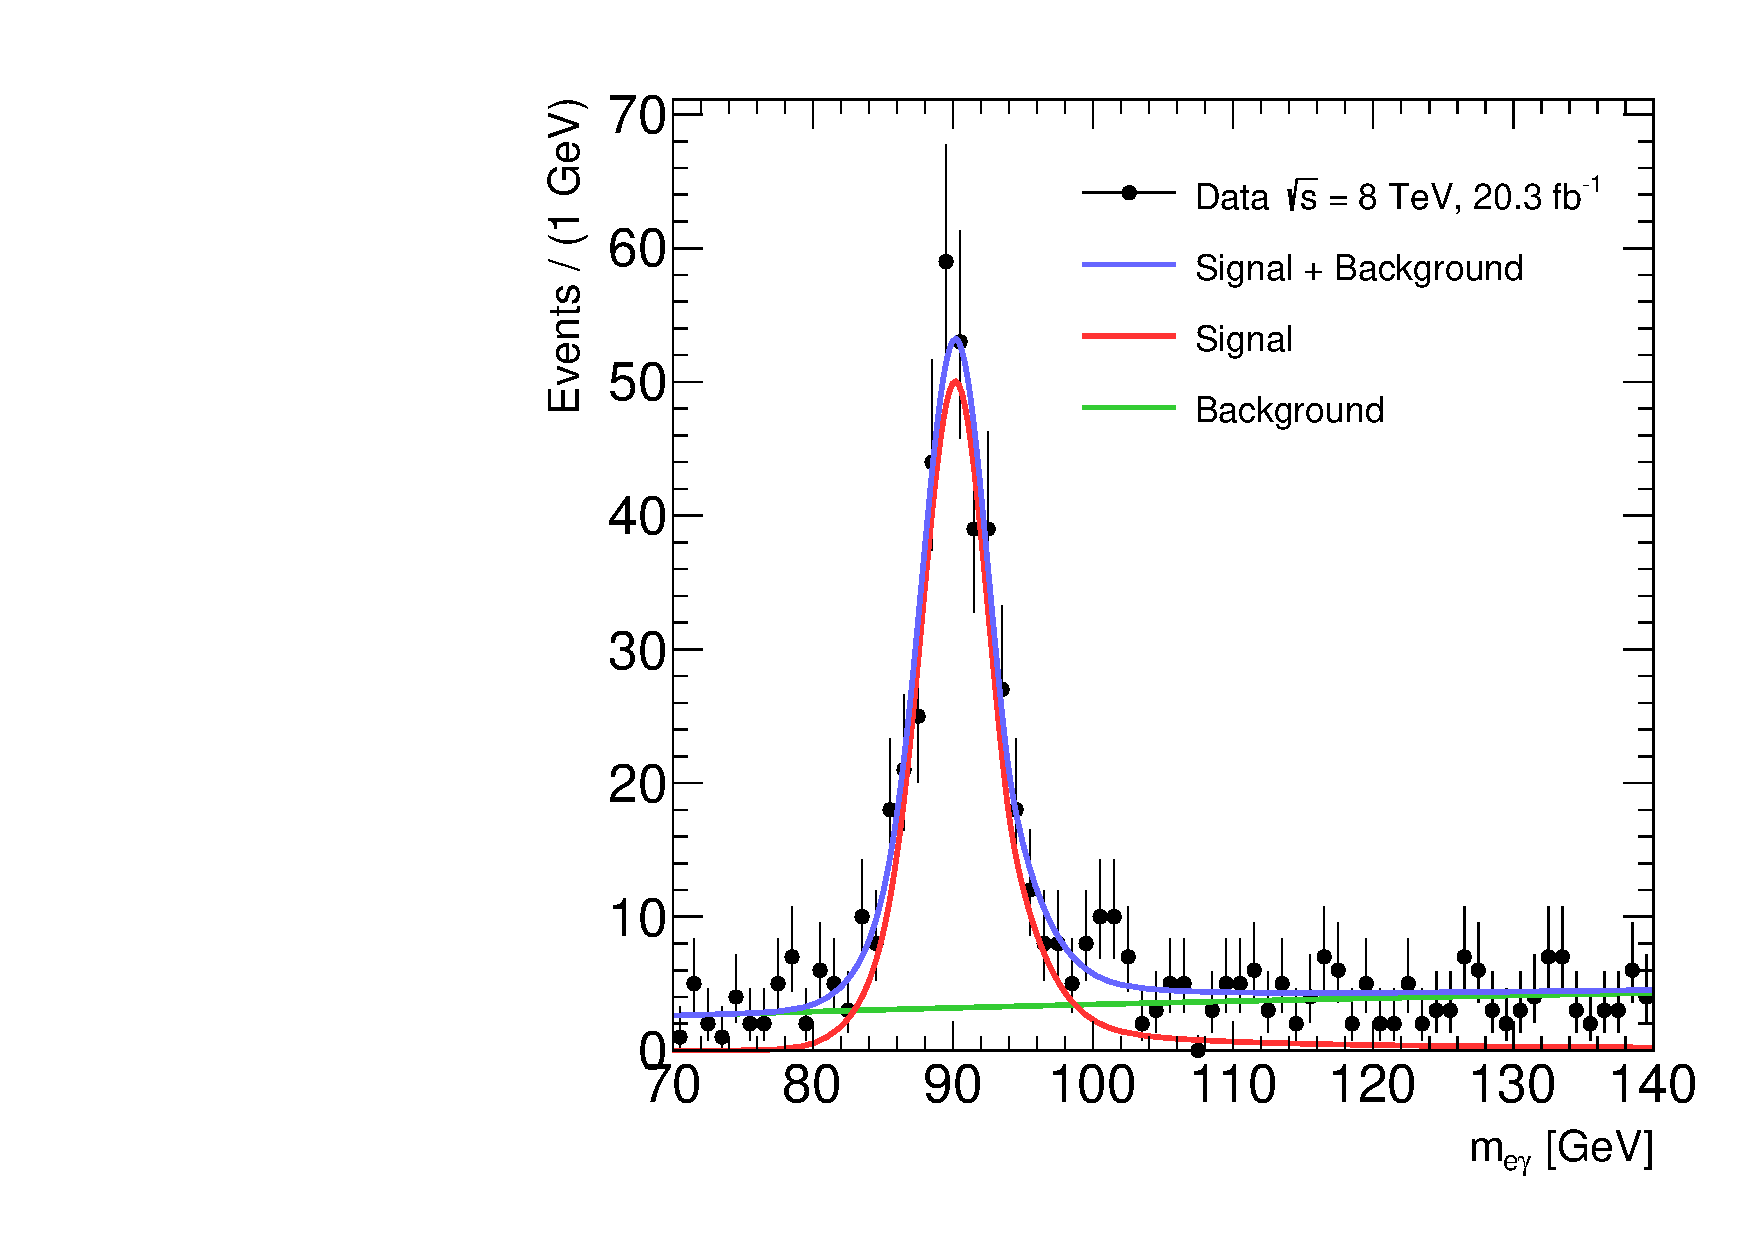
\includegraphics[width=0.49\textwidth]{figures/Fit_meg_efakes_Data_all}
  \caption{Distribuciones de la masa invariante de los pares de
    electrón-electrón (izquierda) y electrón-fotón (derecha). Se puede ver también el ajuste
    con el modelo de señal + fondo.}
  \label{fig:invmass_pairs}

\end{figure}

La probabilidad de identificación errónea se muestra en la \cref{fig:efake_eta},
como función del {\abseta} del objeto \emph{probe} para ``fotones'' convertidos
y no-convertidos. Este factor crece con {\abseta}, lo cual esta relacionado
con el incremento en el material del detector atravesado por los electrones y el
incremento en la tasa de reconstrucción de fotones convertidos con una sola
traza.

El {\feg} calculado a partir de los datos es comparado con el calculado a partir
de muestras MC de eventos de {\Zee} producidas con los generadores {\sherpa} y
{\powheg}. Se encuentra un buen acuerdo para todos los casos dentro de sus incertezas.
Los valores calculados de {\feg} pueden verse en la \cref{tab:efake_eta}, y \cref{tab:efake_uc} para fotones
convertidos y no-convertidos de forma separada.

\begin{figure}[!htbp]
  \centering

  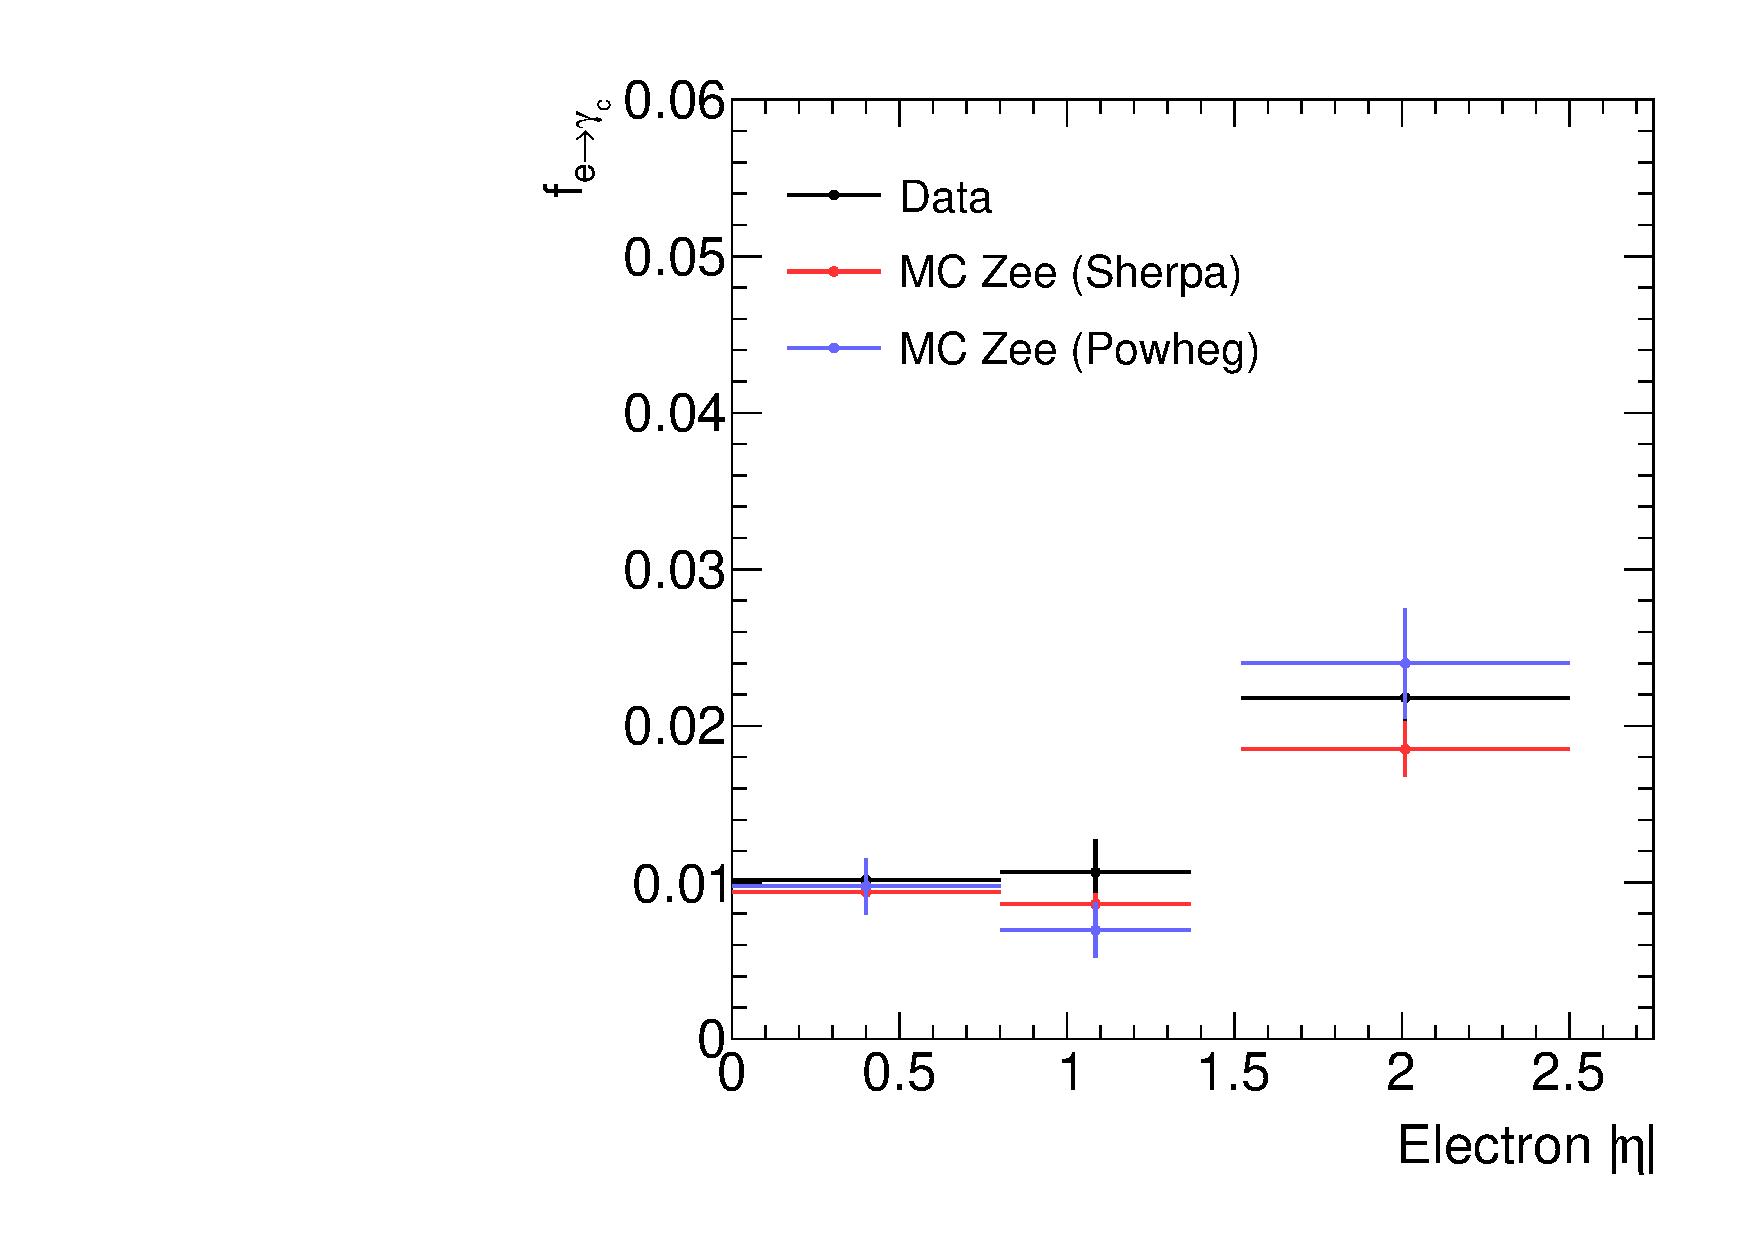
\includegraphics[width=0.45\textwidth]{figures/fegc_feta}
  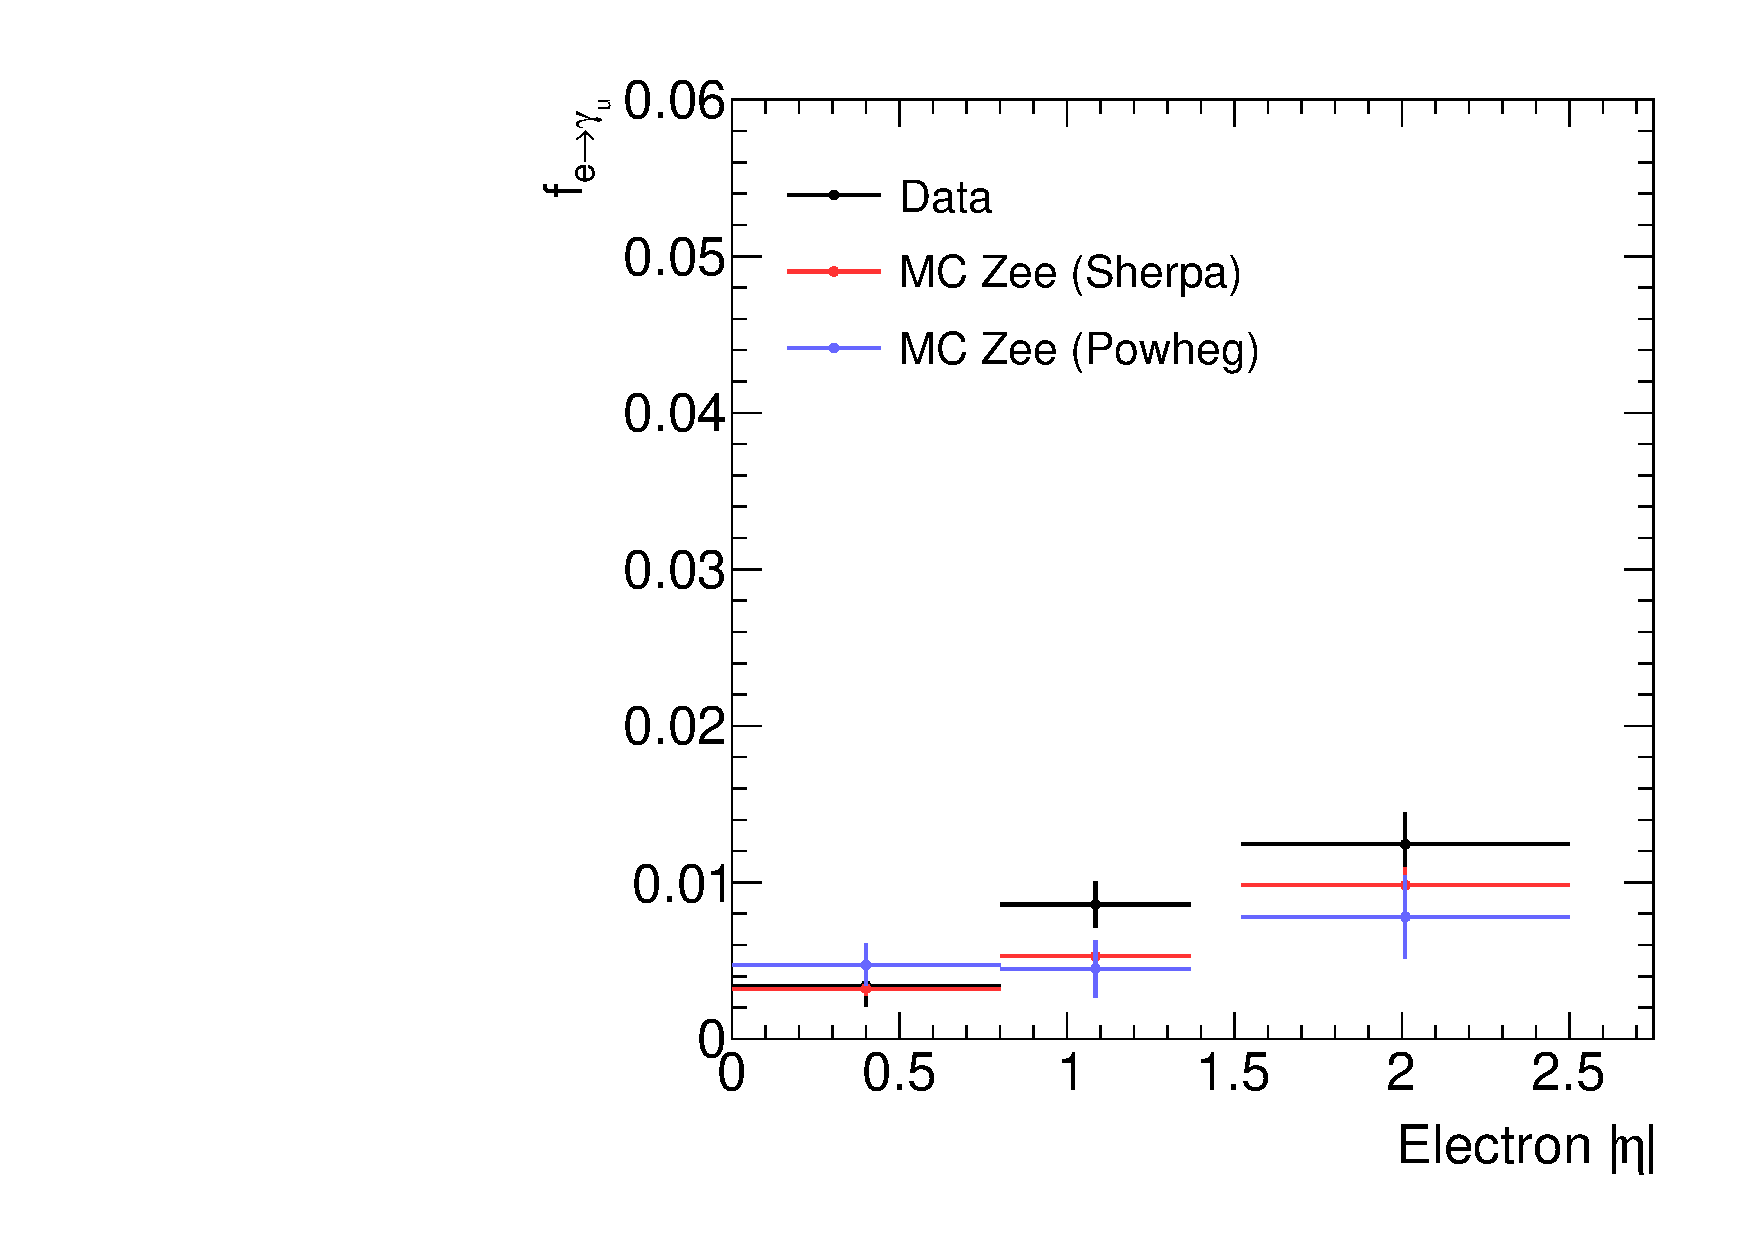
\includegraphics[width=0.45\textwidth]{figures/fegu_feta}

  \caption{Probabilidad de que un electrón real sea identificado como un fotón convertido (izquierda)
    y un fotón no-convertido (derecha), como función de la pseudo-rapidez del objeto \emph{probe}. El valor
    calculado a partir de los datos es comparado con el valor calculado con las muestras MC de eventos de {\Zee} utilizando
    dos generadores distintos.}
  \label{fig:efake_eta}
\end{figure}


\begin{table}[!htbp]
  \centering
  \caption{Probabilidad de que un electrón real sea identificado como un fotón,
    como función de la pseudo-rapidez del objeto \emph{probe}. El valor
    calculado a partir de los datos es comparado con el valor calculado con las
    muestras MC de eventos de {\Zee} utilizando dos generadores distintos.}
  \label{tab:efake_eta}

  %\begin{tabular}{L{0.16\textwidth}x{0.21\textwidth}x{0.21\textwidth}x{0.21\textwidth}}
  \begin{tabularx}{\textwidth}{CCCC}
    \hline
                          & Datos             &  MC {\Zee} (\sherpa) & MC {\Zee} (\powheg) \\
    \hline
    $0 < |\eta| < 0.8$    & $0.014 \pm 0.002$ & $0.012 \pm 0.001$ & $0.014 \pm 0.002$ \\
    $0.8 < |\eta| < 1.52$ & $0.018 \pm 0.003$ & $0.014 \pm 0.001$ & $0.011 \pm 0.003$ \\
    $1.52 < |\eta| < 2.5$ & $0.033 \pm 0.006$ & $0.027 \pm 0.002$ & $0.032 \pm 0.006$ \\
    Inclusivo             & $0.019 \pm 0.001$ & $0.016 \pm 0.001$ & $0.017 \pm 0.002$ \\
    \hline
  \end{tabularx}

\end{table}

\begin{table}[!htbp]
  \centering
  \caption{Probabilidad de que un electrón real sea reconstruido como un fotón
    convertido o no-convertido. El valor calculado a partir de los datos es
    comparado con el valor calculado con las muestras MC de eventos de {\Zee},
    utilizando dos generadores distintos.}
  \label{tab:efake_uc}

%  \begin{tabular}{x{0.16\textwidth}x{0.21\textwidth}x{0.21\textwidth}x{0.21\textwidth}}
  \begin{tabularx}{\textwidth}{CCCC}

    \hline
                       & Datos              & MC {\Zee} (\sherpa)        & MC {\Zee} (\powheg)        \\
    \hline
    $f_{e\to \gamma_u}$ & $0.007 \pm 0.001$ & $0.005 \pm 0.001$ & $0.005 \pm 0.001$ \\
    $f_{e\to \gamma_c}$ & $0.013 \pm 0.001$ & $0.011 \pm 0.001$ & $0.011 \pm 0.002$ \\
    $f_{e\to \gamma}$   & $0.019 \pm 0.001$ & $0.016 \pm 0.001$ & $0.017 \pm 0.002$ \\
    \hline
  \end{tabularx}

\end{table}


Para estimar la incerteza sistemática del método utilizado, el factor {\feg} fue
calculado variando el tamaño de la ventana de masa del $Z$, y sin la sustracción
del fondo. Como se aprecia en la \cref{tab:efake_syst}, en el caso de no
realizar la sustracción del fondo, es donde se obtiene la mayor variación y por
lo tanto se utiliza ese valor como la incerteza sistemática del método, a pesar
de que resulta conservativo.

\begin{table}[!htbp]
  \centering
  \caption{Probabilidad de que un electrón real sea reconstruido como un fotón
    convertido o no-convertido, para variaciones del método original.}
  \label{tab:efake_syst}

  %\begin{tabular}{x{0.14\textwidth}x{0.22\textwidth}x{0.22\textwidth}x{0.22\textwidth}}
  \begin{tabularx}{\textwidth}{CCCC}
    \hline
            &  $m_{ee} \in [71, 111] \GeV$ & $m_{ee} \in [86,96] \gev$ & Sin sustracción del fondo  \\
    \hline
    $f_{e\to \gamma_u}$ & $0.007 \pm 0.001$ & $0.007 \pm 0.001$ & $0.012 \pm 0.001$ \\
    $f_{e\to \gamma_c}$ & $0.013 \pm 0.001$ & $0.012 \pm 0.001$ & $0.012 \pm 0.001$ \\
    $f_{e\to \gamma}$   & $0.019 \pm 0.001$ & $0.019 \pm 0.001$ & $0.024 \pm 0.001$ \\
    \hline
  \end{tabularx}

\end{table}


El valor calculado del factor de identificación errónea de electrón en fotón
({\feg}) resulta entonces el que se muestra en la \cref{tab:efake_final}.

\begin{table}[!htbp]
  \centering

  \caption{Probabilidad de que un electrón real sea reconstruido como un fotón {\feg}, como función de $\eta$, junto
    con su error estadístico y sistemático.}
  \label{tab:efake_final}

  %\begin{tabular*}{0.8\textwidth}{@{\extracolsep{\fill}}cc}
  \begin{tabularx}{0.8\textwidth}{CC}

    \hline
     Región                &  $f(e\to \gamma)$  \\
    \hline
      $0 < |\eta| < 0.8$     & $ \quad  0.014 \pm 0.002 \stat\ \pm 0.005 \syst\ $ \\
      $0.8 < |\eta| < 1.52$  & $ \quad  0.018 \pm 0.003 \stat\ \pm 0.004 \syst\ $ \\
      $1.52 < |\eta| < 2.5$  & $ \quad  0.033 \pm 0.006 \stat\ \pm 0.008 \syst\ $ \\
    \hline
  \end{tabularx}

\end{table}


\hl{Agregar definición de la control sample y numero finales en las SR}

%% FINAL ESTIMATION IN SIGNAL REGIONS
%% \subsubsection{Estimación final en las regiones de señal} \label{sec:efakes_estimation}

%% En la region CSE$_L$, there are 28 events observed, which then correspond to an estimation for this background of $N^\text{SR2}_\text{efakes} = 0.38\, \pm\, 0.07$.
%% In CSE3, given the harder \MET\ cut, there is no observed event in the electron sample for the data analised.

%number of electron events observed by the fake factor computed in data in three $\eta$ regions, [0, 0.8], [0.8, 1.52], [1.52, 2.5].

%% In SR2, only one electron event is observed, which then correspond to an estimation for this background of $N^\text{SR2}_\text{efakes} = 0.02\, \pm\, 0.02$.
%% In SR3, given the harder \MET\ cut, there is no observed event in the electron sample for the data analised.
%% The MC predicts this background to be indeed rather small (actually no event survived the SR3 selection with
%% the available statistics), which is consistent with the observed limit of $<0.02$ events. The estimation of
%% electron fake background for SR3 is then $N^\text{SR3}_\text{efakes} = 0.0^{+0.03}_{-0.0}$, which accomodates the total fake rate uncertainty.

%As a conservative estimate, the last observed yield in the \MET distribution (one event at 200\gev) is taken. This way, it translates to the same estimation as for SR2, after the \etogam\ fake factor is applied.


%The total number of electron events, summed over all $\eta$ bins is reported in \Tab \ref{tab:efake_yields}.
%From these, the number of \etogam\ events expected in the signal region is %$3.679\pm xx$,
%$0.828\pm yy$ and $0.679\pm zz$ events for SR2 and SR3 signal regions, respectively. Only statistical uncertainties are here considered. \tosolve{uncertainties!}%%The associated systematics are discussed in sec \ref{sec:syst_efakes}.
%
%\begin{table}[h!]
%  \centering
%    \caption{Number of misidentified electron events expected in the different signal regions. The unscaled number is weighted by
%    the electron-photon fake rate to get the final background yield from electron fakes in the three
%  analysis regions.}
%  \begin{tabular}{c|cc}
%    \hline
%    \hline
%    Signal region & Unscaled & Weighted  \\
%    \hline
%%    SR1 & $231$ & $3.679$ \\ %% \pm 0.251$ \\
%    SR2 & $57$ & $0.828$ \\ %% \pm 0.110$ \\
%    SR3 & $47$ & $0.679$ \\ %% \pm 0.100$ \\
%    \hline
%    \hline
%  \end{tabular}
%  \label{tab:efake_yields}
%\end{table}




%-----------
% Jet fakes
%-----------
\section{Jets identificados como fotones} \label{sec:jetfakes}

Los jets pueden ser identificados como fotones si fluctúan a uno o dos
{\pizero} con alto \pt, resultando en un objeto electromagnético indistinguible
de un solo fotón muy energético. Este fondo proviene mayoritariamente de
multijets, {\wjets} y eventos {\ttbar} decayendo semi-leptónicamente, y puede
ser una fuente importante de contaminación. Como la proporción de jets mal
identificados como fotones no esta bien descripta por el MC, se la determina
utilizando un método a partir de los datos. La idea es utilizar las diferencias
en la distribución de energía de aislamiento esperada para fotones reales y
falsos, como se describe a continuación.

\subsection{Descripción del método}

Para reducir significativamente el fondo proveniente de jets, en el análisis
se utilizan fotones se satisfacen un criterio de selección \emph{tight}, como se
describe en \cref{sec:pho_obj}. Esta selección es inclusiva respecto a los
fotones reales y tienen una moderada contaminación de jets. Es por definición un
criterio mas ajustado que el trigger de fotones utilizado para la toma de los
datos, por lo que hay una suficiente cantidad de candidatos a fotones provenientes de jets
que fallan la selección \emph{tight} pero satisfacen una selección
intermedia. Estos jets más similares a un fotón real, llamados
\emph{pseudo-fotones}, son útiles para modelar los jets que pasan la selección
total y la tasa de esta contaminación.

%Pseudo-photons are here defined as those passing the loose identification
%but failing (at least) one of a set of tight identification cuts. %, also known as {\it loose'-non-tight}.

La muestra de fotones que pasan los criterios de selección \emph{tight}
($N_\text{tight}$) contiene, en general, fotones reales ($N_{\gamma}$) y falsos
($N_{j\to\gamma}$). Las distribuciones de la energía de aislamiento para estas
dos contribuciones van a tener formas diferentes, lo cual puede ser explotado
para estimar ambas contribuciones. Para hacer esto se ajusta la distribución
total de energía de aislamiento con un combinación de modelos de señal y fondo.

%% , tambien
%% tomado de los datos como se explica en
%% \cref{sec:jfake_sig_template,sec:jfake_bkg_template}.

El número de eventos de fotones falsos que pasa la identificación de fotones y
el corte de aislamiento puede ser estimado entonces integrando la componente de
fondo del ajuste sobre el rango de la región de señal ($\etiso<5\GeV$). De esta
forma la proporción de jets mal identificados como fotones, \fjg, resulta:

\begin{equation}\label{eq:jfake_formula}
  f_{j\to \gamma} = \frac{\int_{-\infty}^{5\gev} B(x)\, dx}{\int_{-\infty}^{5\gev} \left[S(x)+B(x)\right]\, dx}
\end{equation}
%
donde $x$ es la variable de energía de aislamiento \etiso, y $S(x)$ y $B(x)$
son las distribuciones de señal y fondo en el ajuste combinado, respectivamente.
Esta fracción de fotones falsos es estimada en una región de control, y luego
utilizada para pesar la muestra de fotones en la SR para estimar el número de
eventos provenientes de jets mal identificados. Este resultado se discute en
\cref{sec:jet_fake_results}.



\subsection{Modelo de Señal} \label{sec:jfake_sig_template}

El modelo de señal se extrajo de eventos de datos {\Zee} usando el hecho que los
electrones y fotones tienen una señal similar en el calorímetro
electromagnético. La muestra de electrones es obtenida de eventos que satisfacen
el siguiente conjunto de cortes, después de haber pasado la preselección
descripta en \cref{sec:event_baseline}:

\begin{itemize}\itemsep0.1cm
\item Trigger de electrones (\texttt{2e12Tvhi\_loose1} \texttt{e24vhi\_medium1} o
  \texttt{e60\_medium1}).
\item Dos electrones \emph{medium}, aislados, y con carga opuesta, uno con $\pt>50\gev$
  y otro $\pt>25 \gev$
\item \MET\ $<40\gev$
\item $81\gev<m_{ee}<101\gev$
\end{itemize}

Después de aplicar los cortes anteriores, la contaminación de fondos no
provenientes del decaimiento del $Z$ es despreciable, en particular para eventos
de {\ttbar} resulta menor al $1\%$.

\begin{figure}[!htbp]
  \centering
  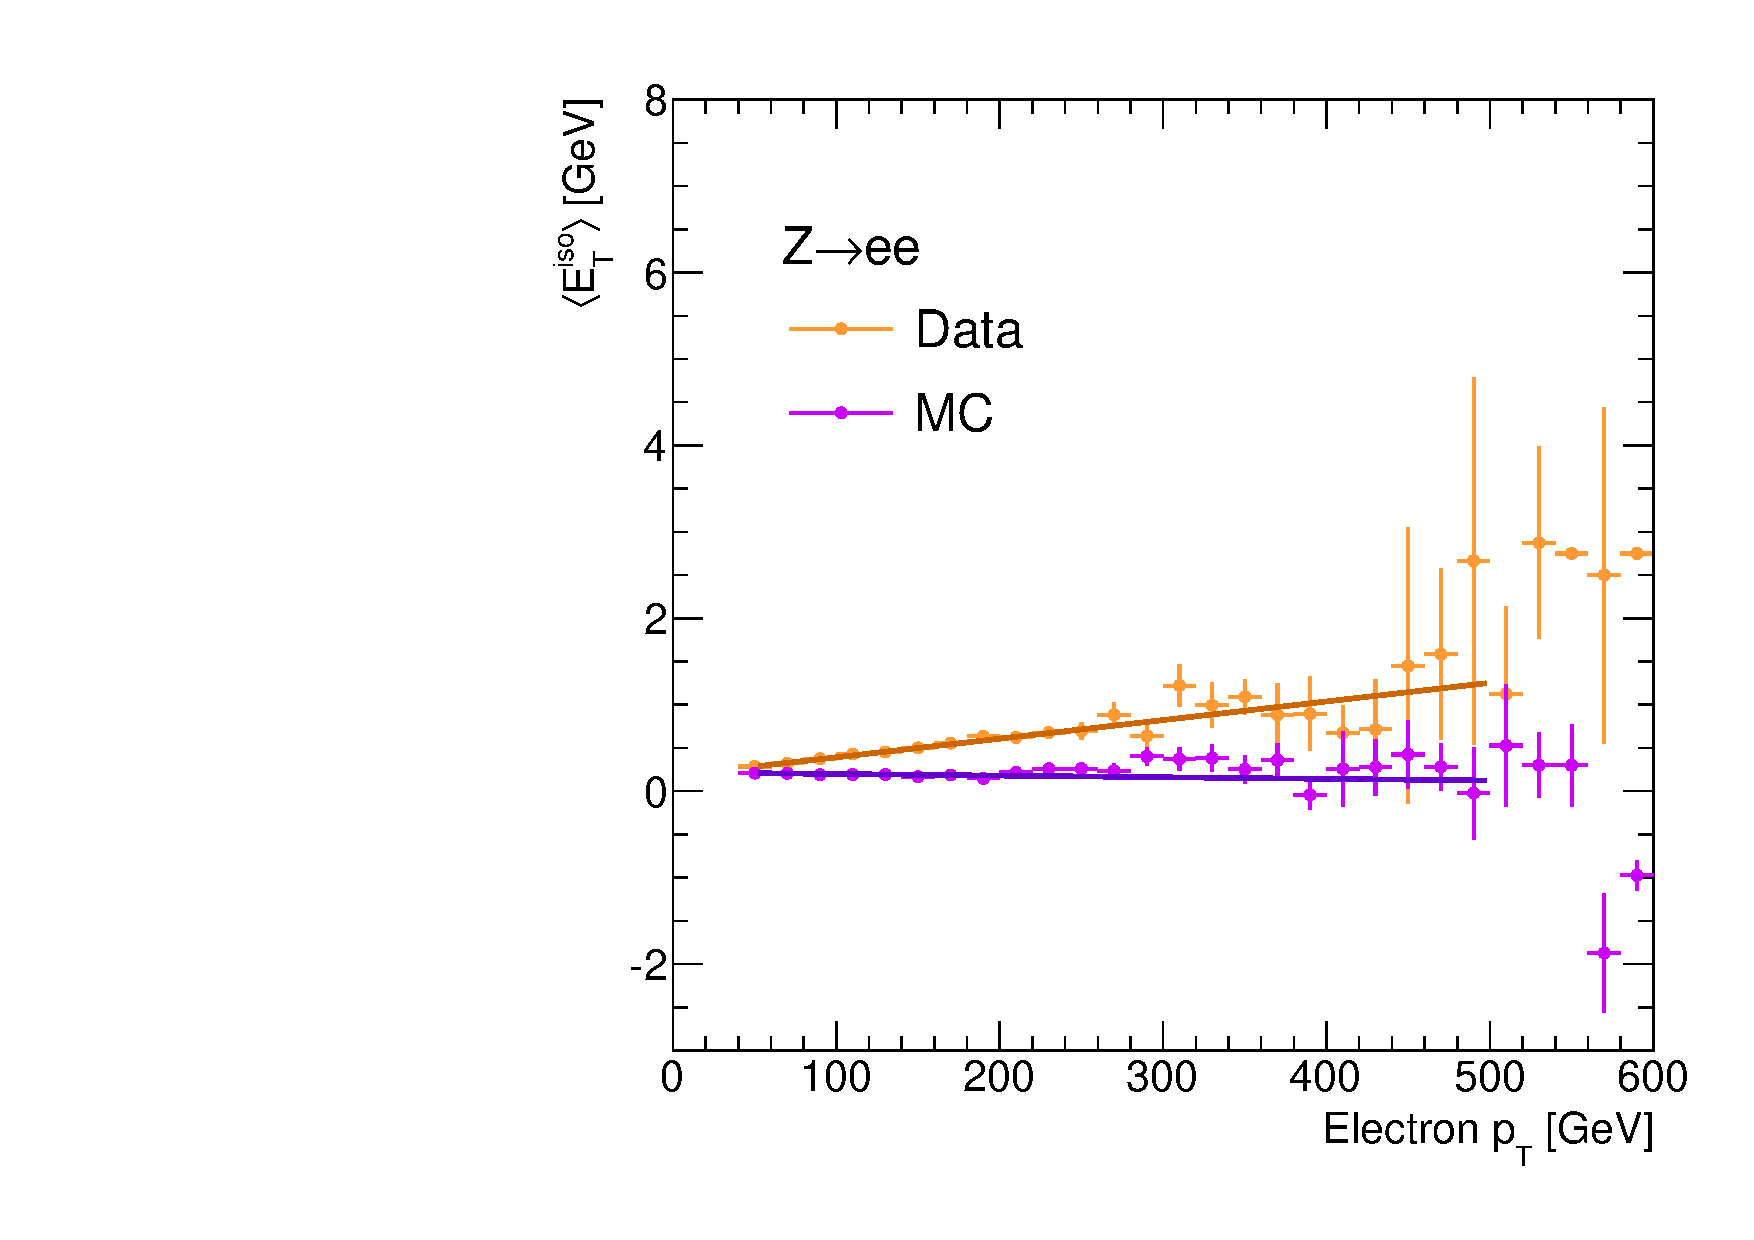
\includegraphics[width=0.49\textwidth]{electron_iso_vs_pt_Zee_raw}

  \caption{Distribución de {\etiso} para electrones vs. {\pt} de eventos {\Zee} en datos y MC.}
  \label{fig:isolation_vs_pt}
\end{figure}

La \cref{fig:isolation_vs_pt} muestra la el valor medio de distribución de la energía de
aislamiento para los electrones seleccionados, como función del {\pt} del
electrón en eventos de datos y simulaciones MC. De la figura es evidente que
para los datos existe una clara dependencia de {\etiso} con {\pt}, aunque no se
aprecia para las simulaciones MC.
Para corregir esta dependencia residual con {\pt} se realiza un ajuste lineal de los
datos del cual se obtiene un factor de corrección que luego es aplicado a {\etiso}.
El valor del factor de corrección
obtenido en el ajuste en el rango $50<\pt<500 \gev$ es $0.00262 \pm 0.00008$.
Conviene notar que este factor es solo aplicado para corregir los datos.

En la
\cref{fig:isolation_wandwo_correction} se muestra una comparación entre datos y
simulaciones del perfil de {\etiso} antes (izquierda) y después (derecha) de
la corrección. Se puede ver que el acuerdo entre datos y MC es mucho mejor después
de aplicar la corrección.


\begin{figure}[!htbp]
  \centering

  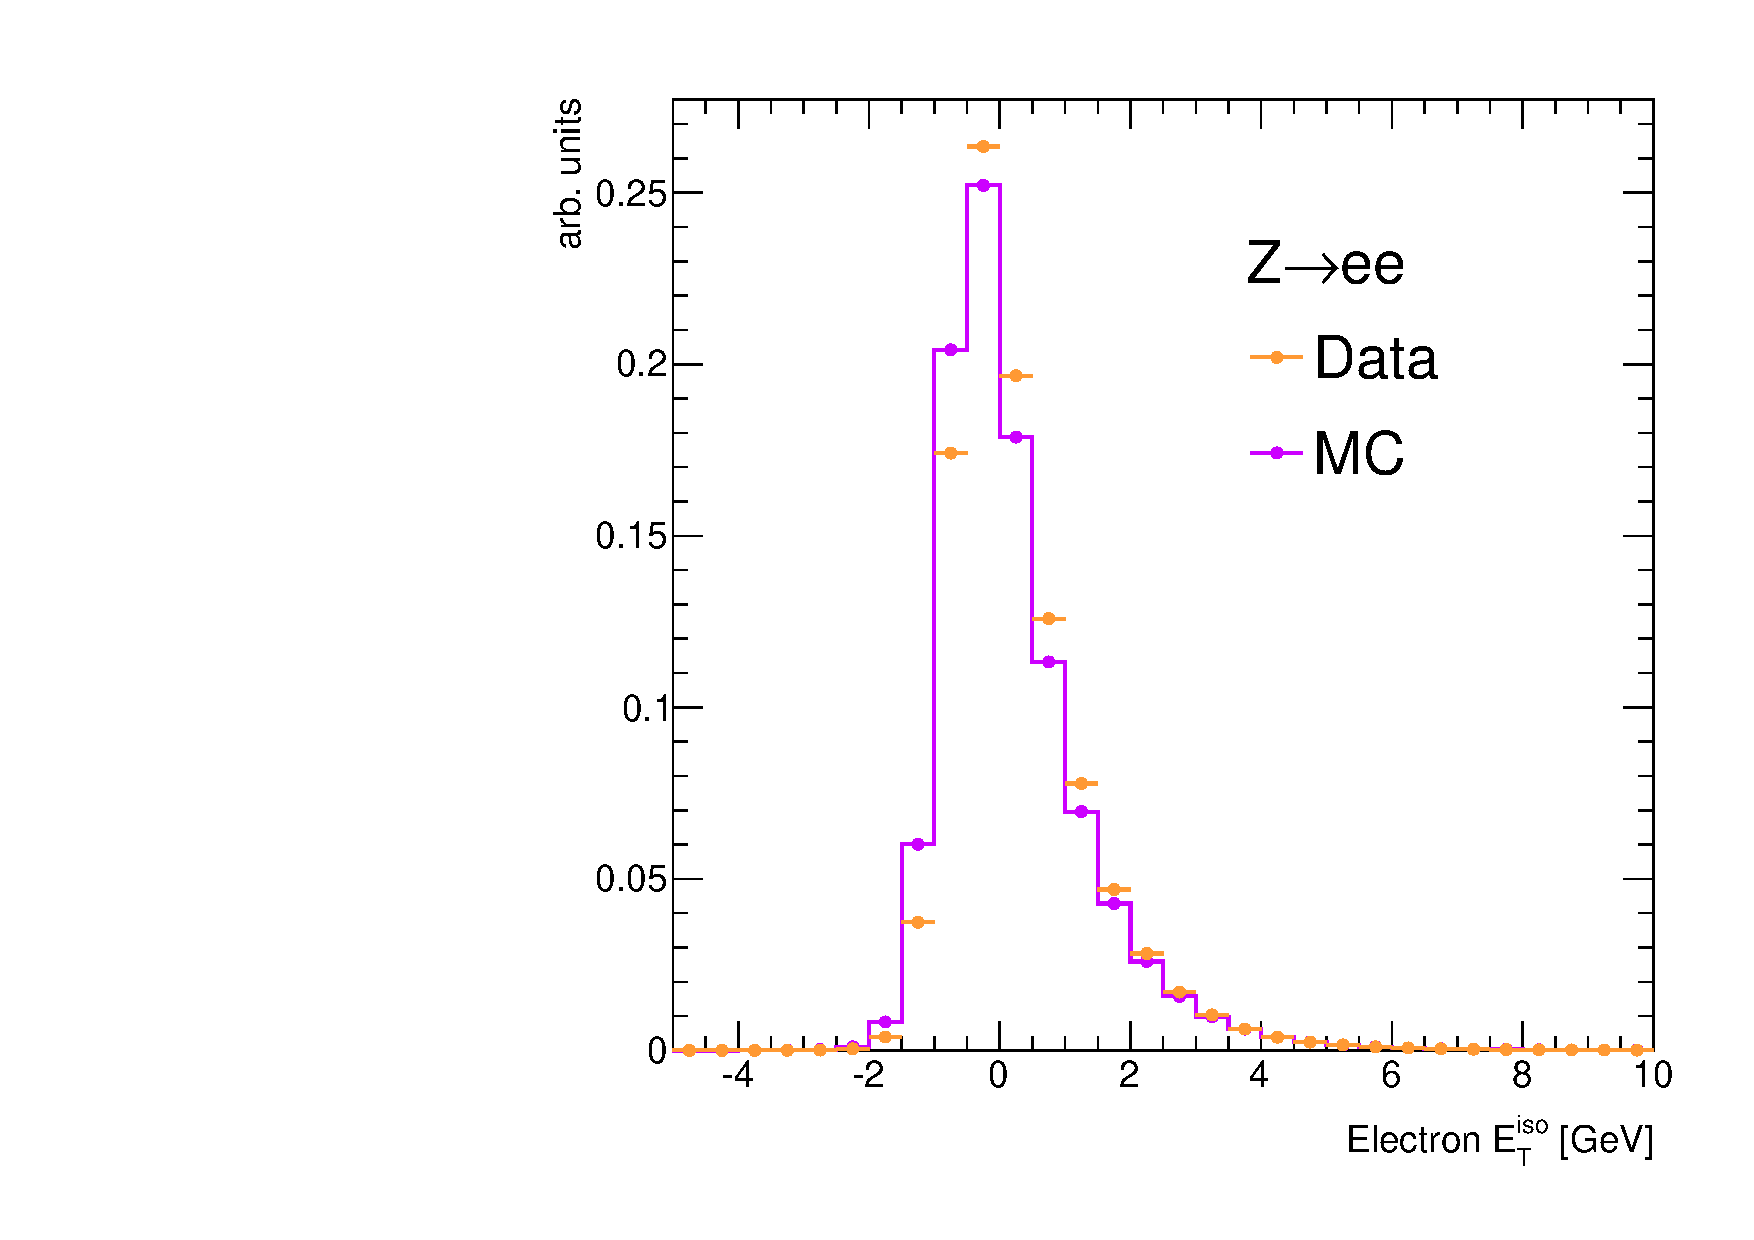
\includegraphics[width=0.49\textwidth]{electron_iso_Zee_raw}
  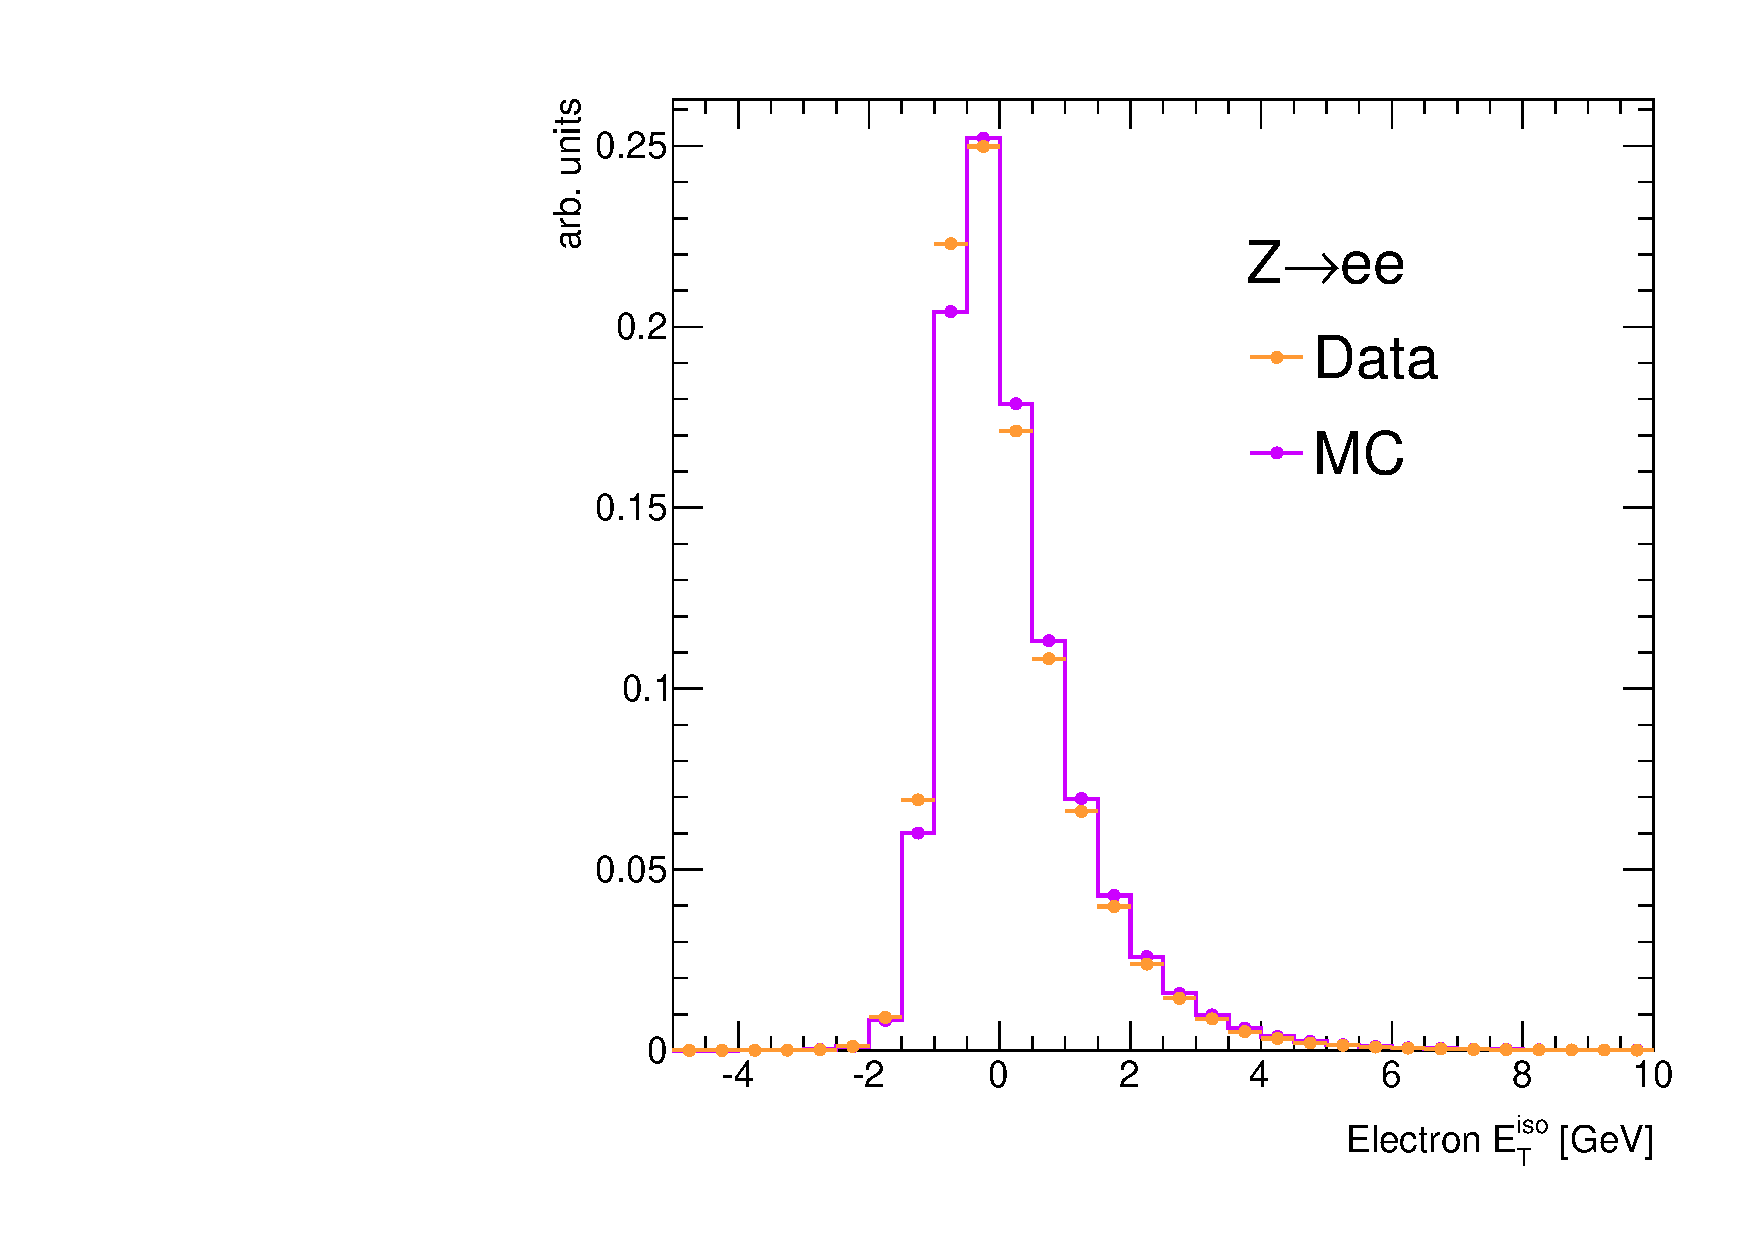
\includegraphics[width=0.49\textwidth]{electron_iso_Zee_corr}

  \caption{Comparación datos/MC de la distribución de {\etiso} de electrones
    provenientes de eventos {\Zee} (izquierda) y la correspondiente distribución
    después de aplicar la corrección por el {\pt} (derecha).}
  \label{fig:isolation_wandwo_correction}
\end{figure}


Para respaldar la estrategia de derivar el modelo de aislamiento de los fotones
de electrones se realizaron varios estudios. Una validación importante del método
consistió en comparar la distribución de {\etiso} de electrones provenientes de
{\Zee} con los fotones provenientes del decaimiento radiativo del $Z$ (\Zee\gam) que provee un fuente
de fotones puros. Los eventos se seleccionaron requiriendo el siguiente conjunto
de cortes, después de la preselección:

\begin{itemize}\itemsep0.1cm
\item Triggers de electrones (\texttt{2e12Tvhi\_loose1} o \texttt{e24vhi\_medium1} o \texttt{e60\_medium1})
\item Un fotón \emph{tight} aislado con $\pt>25 \gev$.
\item Dos electrones \emph{medium}, aislados, con carga opuesta, y con $\pt>50 \gev$ y $\pt>25 \gev$
\item $\Delta R(\gamma,l)>0.7$
\item \MET\ $<40\gev$
\item $40\gev<m_{ee}<85\gev$
\item $70\gev<m_{ee\gamma}<100\gev$
\end{itemize}

En la \cref{fig:photon_electron_iso} se presenta una comparación entre el modelo
de fotones reales de decaimientos radiativos del $Z$ y electrones de {\Zee}. El
gráfico a la derecha es obtenido después de remover la dependencia con el {\pt}
con el factor de corrección como se describió anteriormente. Puede verse
el buen acuerdo entre las distribuciones de {\etiso} de fotones y
electrones, en particular después de aplicar la corrección, dando confianza en la
hipotesis de usar electrones para modelar los fotones.

%% Vale la pena nota que el espectro de {\pt} de fotones tan bajo en estos
%% procesos (ver {\fig} \ref{fig:zllg_pt}) as compared to the generally broader electron \pt\ spectrum from Z decay. %of the electrons (see {\fig} \ref{fig:zeeg_pt}). \tosolve{add this last plot}

\begin{figure}[!htbp]
  \centering

  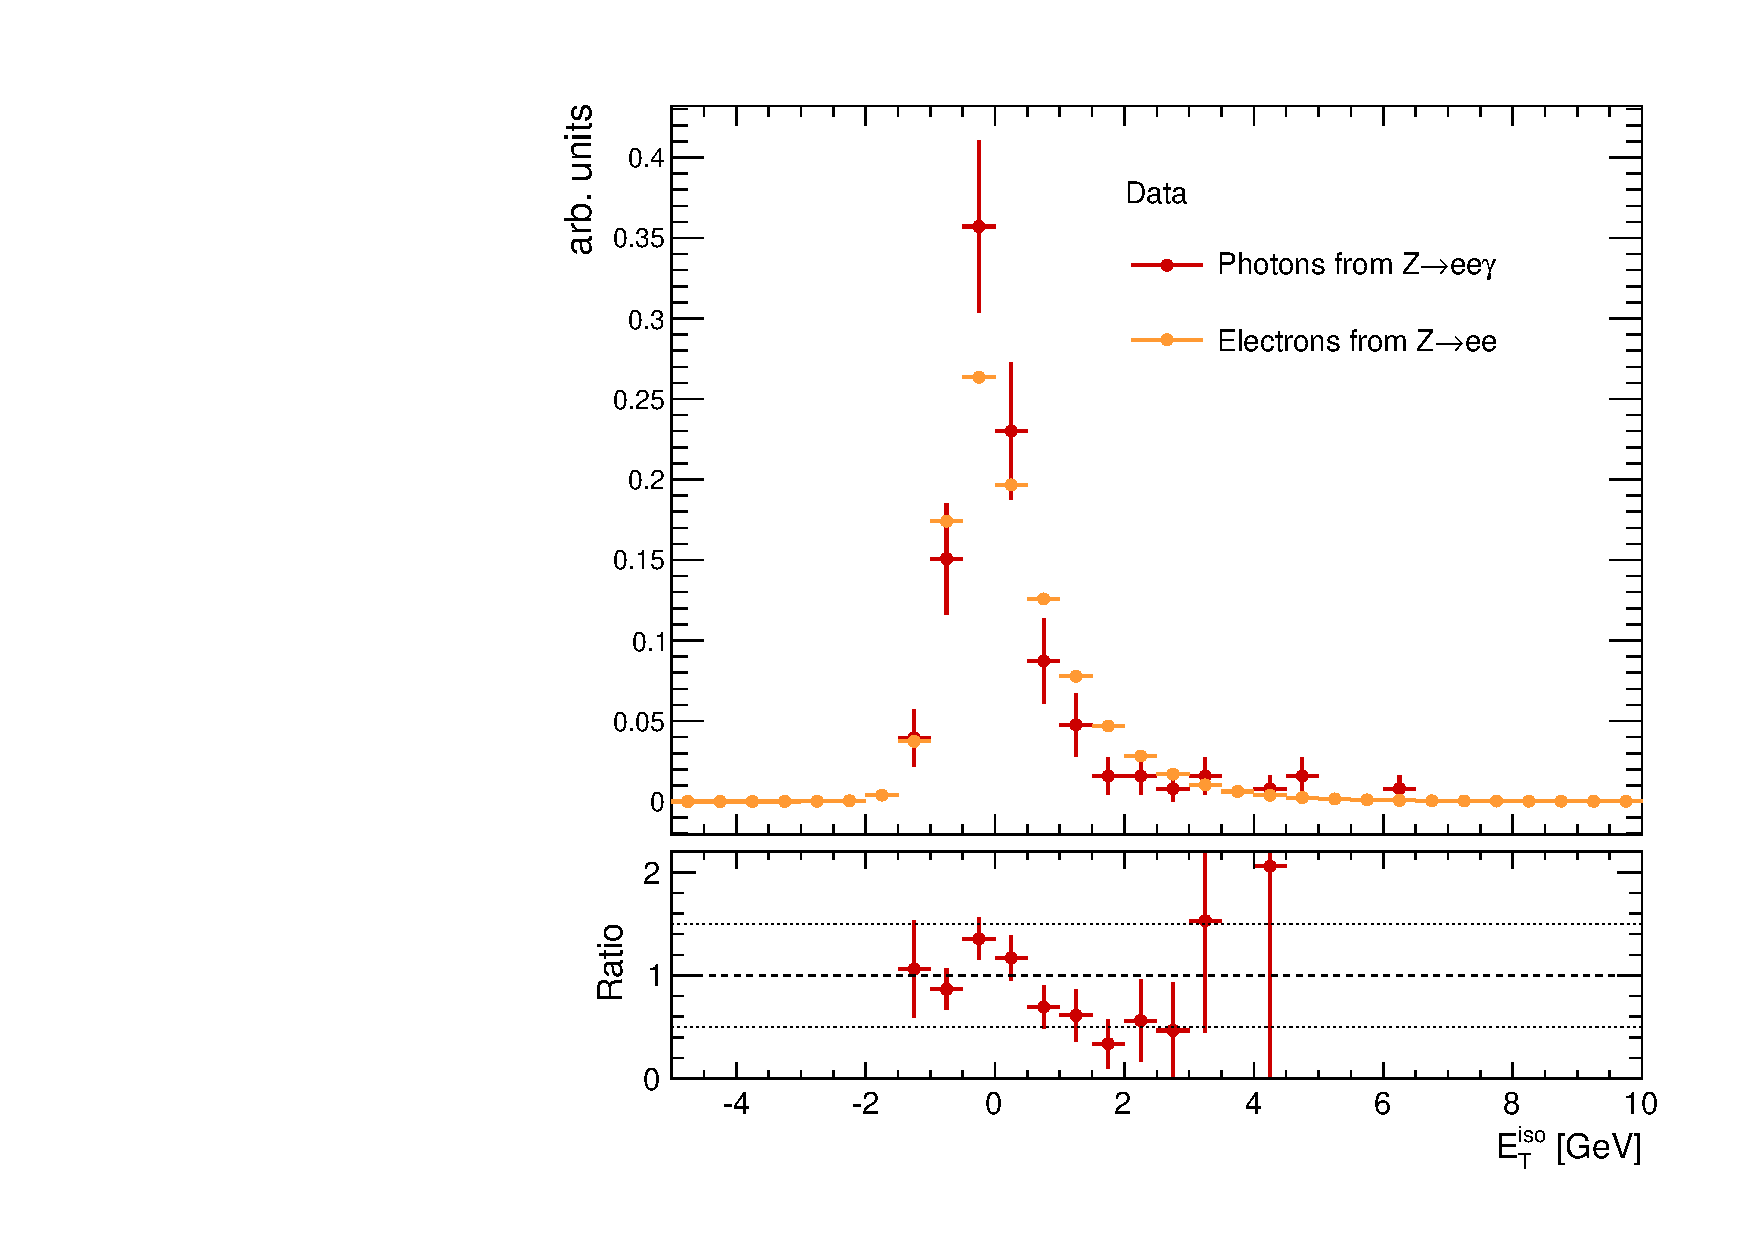
\includegraphics[width=0.49\textwidth]{electronphoton_iso_Zee_before_correction}
  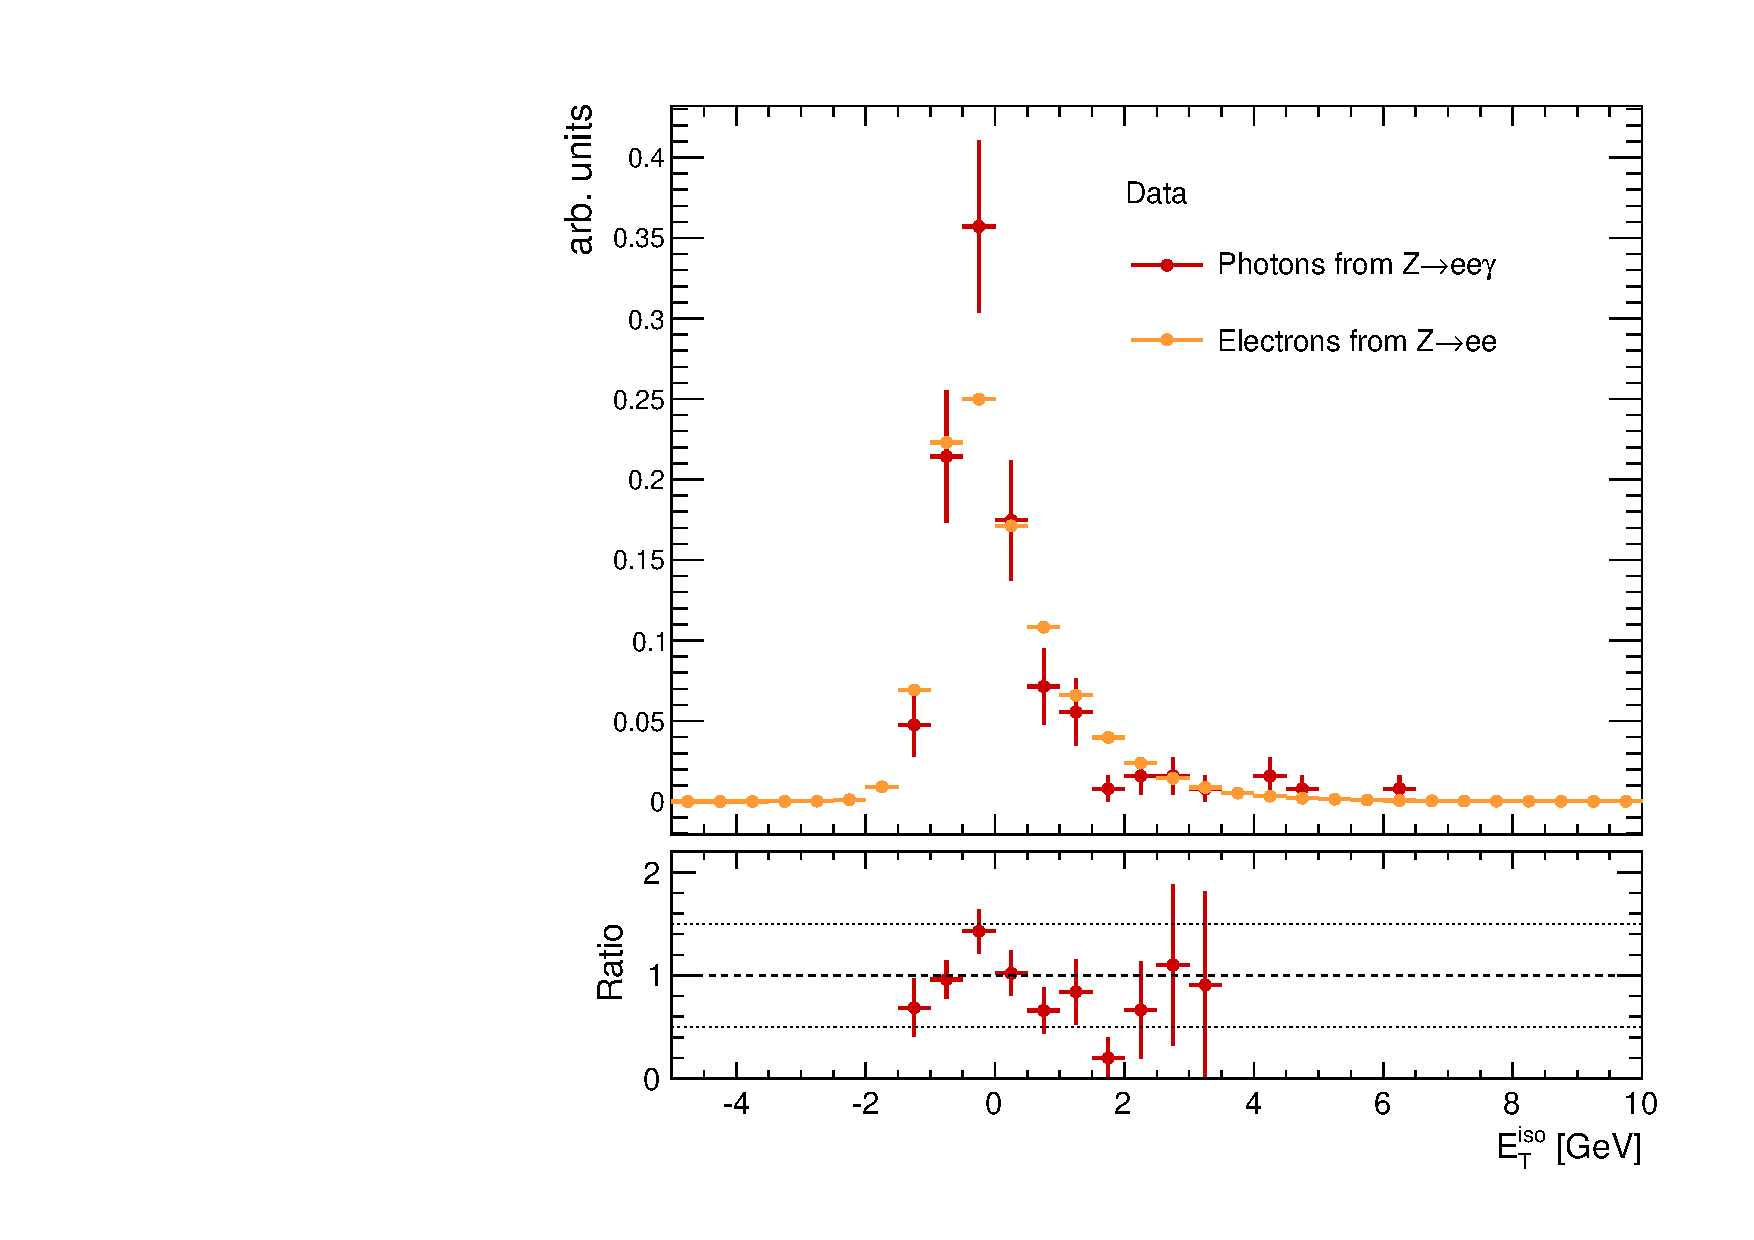
\includegraphics[width=0.49\textwidth]{electronphoton_iso_Zee_after_correction}

  \caption{Comparación de las distribuciones de la energía de aislamiento para fotones reales de
    decaimiento radiativo del $Z$ y electrones provenientes del decaimiento $\Zee$ antes (izquierda)
    y después (derecha) de la corrección por \pt.}
    \label{fig:photon_electron_iso}

\end{figure}

%% \begin{figure}[!htbp]
%%   \centering

%%   \includegraphics[width=0.49\textwidth]{figures/pt_sig_templates}

%%   \caption{Espectro del impulso transverso de fotones provenientes de decaimientos
%%     radiativos del Z, en datos.}
%%   \label{fig:zllg_pt}

%% \end{figure}

Para estudiar el efecto en las distribuciones obtenidas de {\Zee} en distintas
regiones cinemáticas, en \cref{fig:electron_iso_HT}, se presentan las
distribuciones agregando un corte en {\HT} para muestras MC y datos {\Zee}. Como
es de esperar la energía de aislamiento es mas alta y la distribución se hace
mas ancha con \HT.
Desafortunadamente, la escasa estadística impide el uso del corte en {\HT} de la
SR. En cualquier caso, el efecto se considera como una posible fuente de
incerteza sistemática.

\begin{figure}[!htbp]
  \centering

  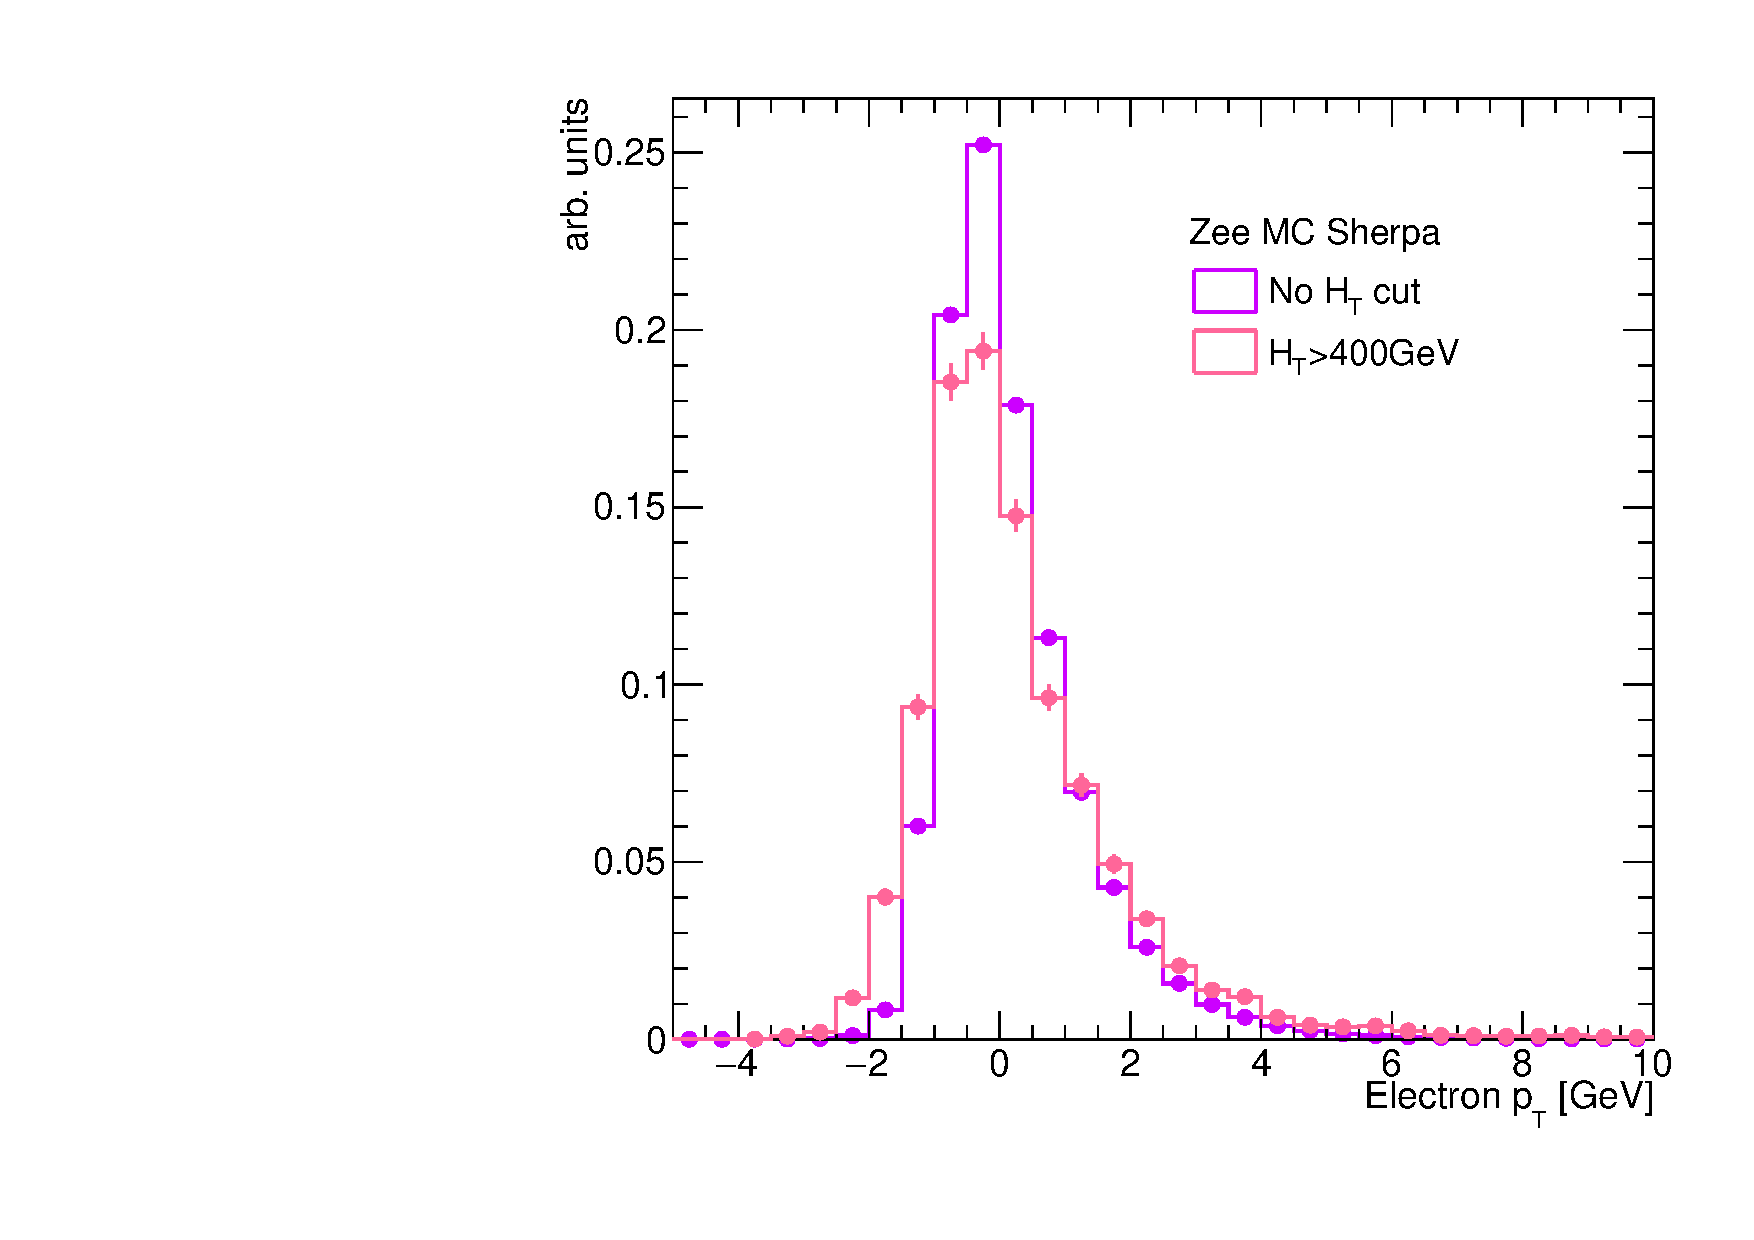
\includegraphics[width=0.49\textwidth]{figures/electron_iso_ZeeHMC_corr}
  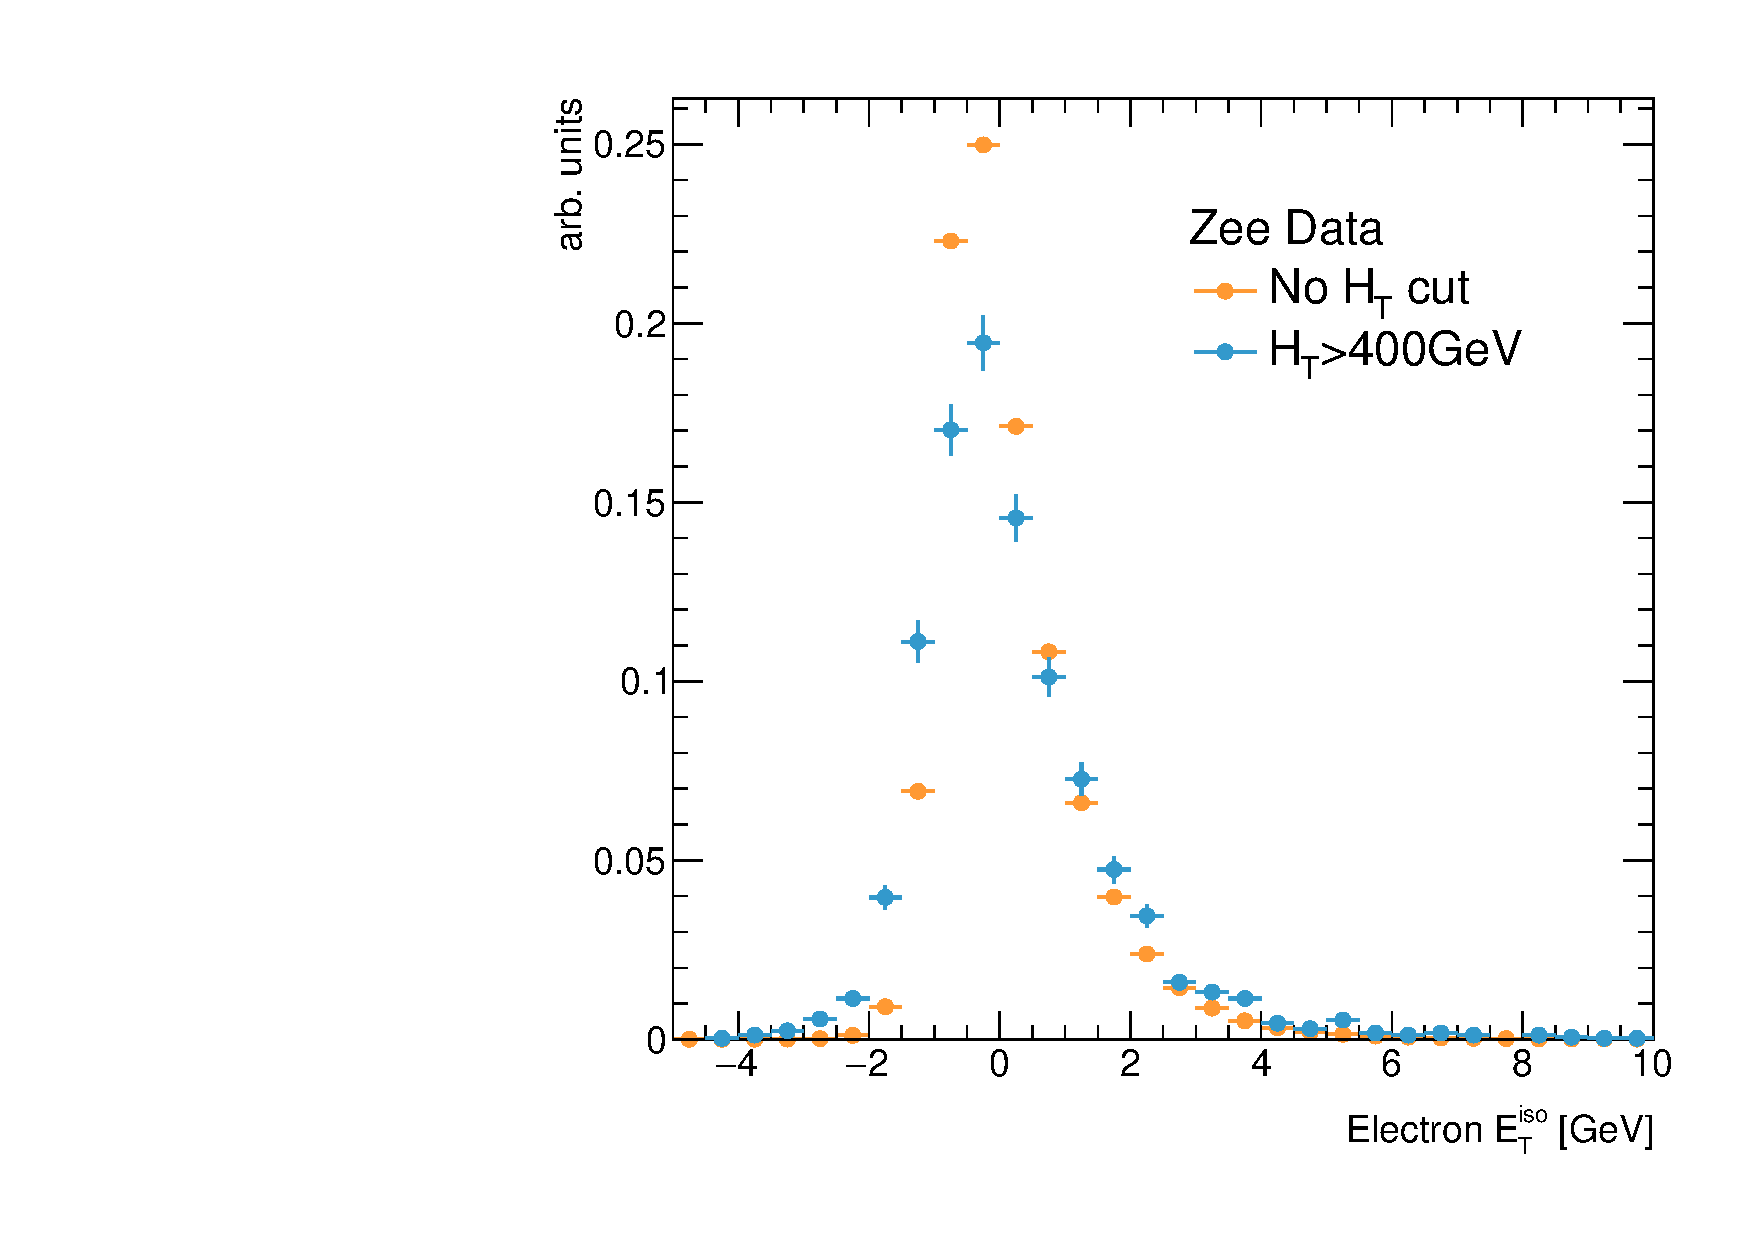
\includegraphics[width=0.49\textwidth]{figures/electron_iso_ZeeH_corr}

  \caption{Dependencia de la energía de aislamiento de electrones con {\HT}
    para MC (izquierda) y datos (derecha) \Zee}
    \label{fig:electron_iso_HT}

\end{figure}



\subsection{Modelo de fondo} \label{sec:jfake_bkg_template}

El modelo de fondo fue derivado de los datos, en eventos que pasan todos los
criterios de identificación salvo los criterios de identificación \emph{tight}
de fotones. La muestra de pseudo-fotones seleccionada de esta forma debe
presentar un perfil de aislamiento similar a la de fotones reales, permitiendo
una pequeña contaminación de señal y alta estadística.

Se realizó un estudio delicado en muestras MC para encontrar el mejor conjunto
de los cortes utilizados por el criterio de identificación \emph{tight} que debía ser
revertido para modelar de la mejor manera la distribución de aislamiento para
los fotones falsos provenientes de decaimientos de hadrones en la SR. En la
\cref{fig:jetfake_mc_data} se puede ver la comparación de dos definiciones
distintas de pseudo-fotones para MC y datos.

%% The background template was derived from the data, in events passing all signal requirements
%% but the tight photon ID cuts. The pseudo-photon sample selected this way should present an
%% isolation profile similar to that for the signal photons, allowing a low signal contamination
%% and high statistics.

%% A dedicated study was done in MC to find the best set of tight ID cuts
%% to be reversed, in order to best model the expected isolation distribution for true hadronic fakes in the SR.
%% This is shown in {\fig} \ref{fig:jetfake_mc_data}, compared to the pseudo-photon sample in MC and data,
%% for two different ID definitions.

Los pseudo-fotones \emph{loose-non-tight} (LNT) pasan los cortes de
identificación \emph{loose}, pero fallan al menos uno de los cortes
\emph{tight}. A pesar de la escasa estadística, resulta claro falla en su
objetivo de modelar el fondo tanto en datos como en MC. Se obtiene un mejor
acuerdo para la definición \emph{loose'-non-tight} (L'NT), en la cual los
fotones pasan todos los cortes \emph{tight} salvo (al menos) uno de las
variables en las narrow strips ($F_\text{side}$, $w_{s3}$, $E_\text{ratio}$,
$\Delta E$). Estas variables son construidas con solo algunas strips centrales
alrededor de la dirección del fotón, y por lo tanto se espera que no tengan una
correlación con la energía de aislamiento del fotón, ya que para el calculo de
esta se excluye la energía en las celdas centrales para tener en cuenta la
propia energía del fotón. Utilizando esta definición, los pseudo-fotones tiene
un perfil de aislamiento con una forma similar a la de fotones \emph{tight} y
por lo tanto es posible la extrapolación a la SR.

\begin{figure}[!htbp]
  \centering

  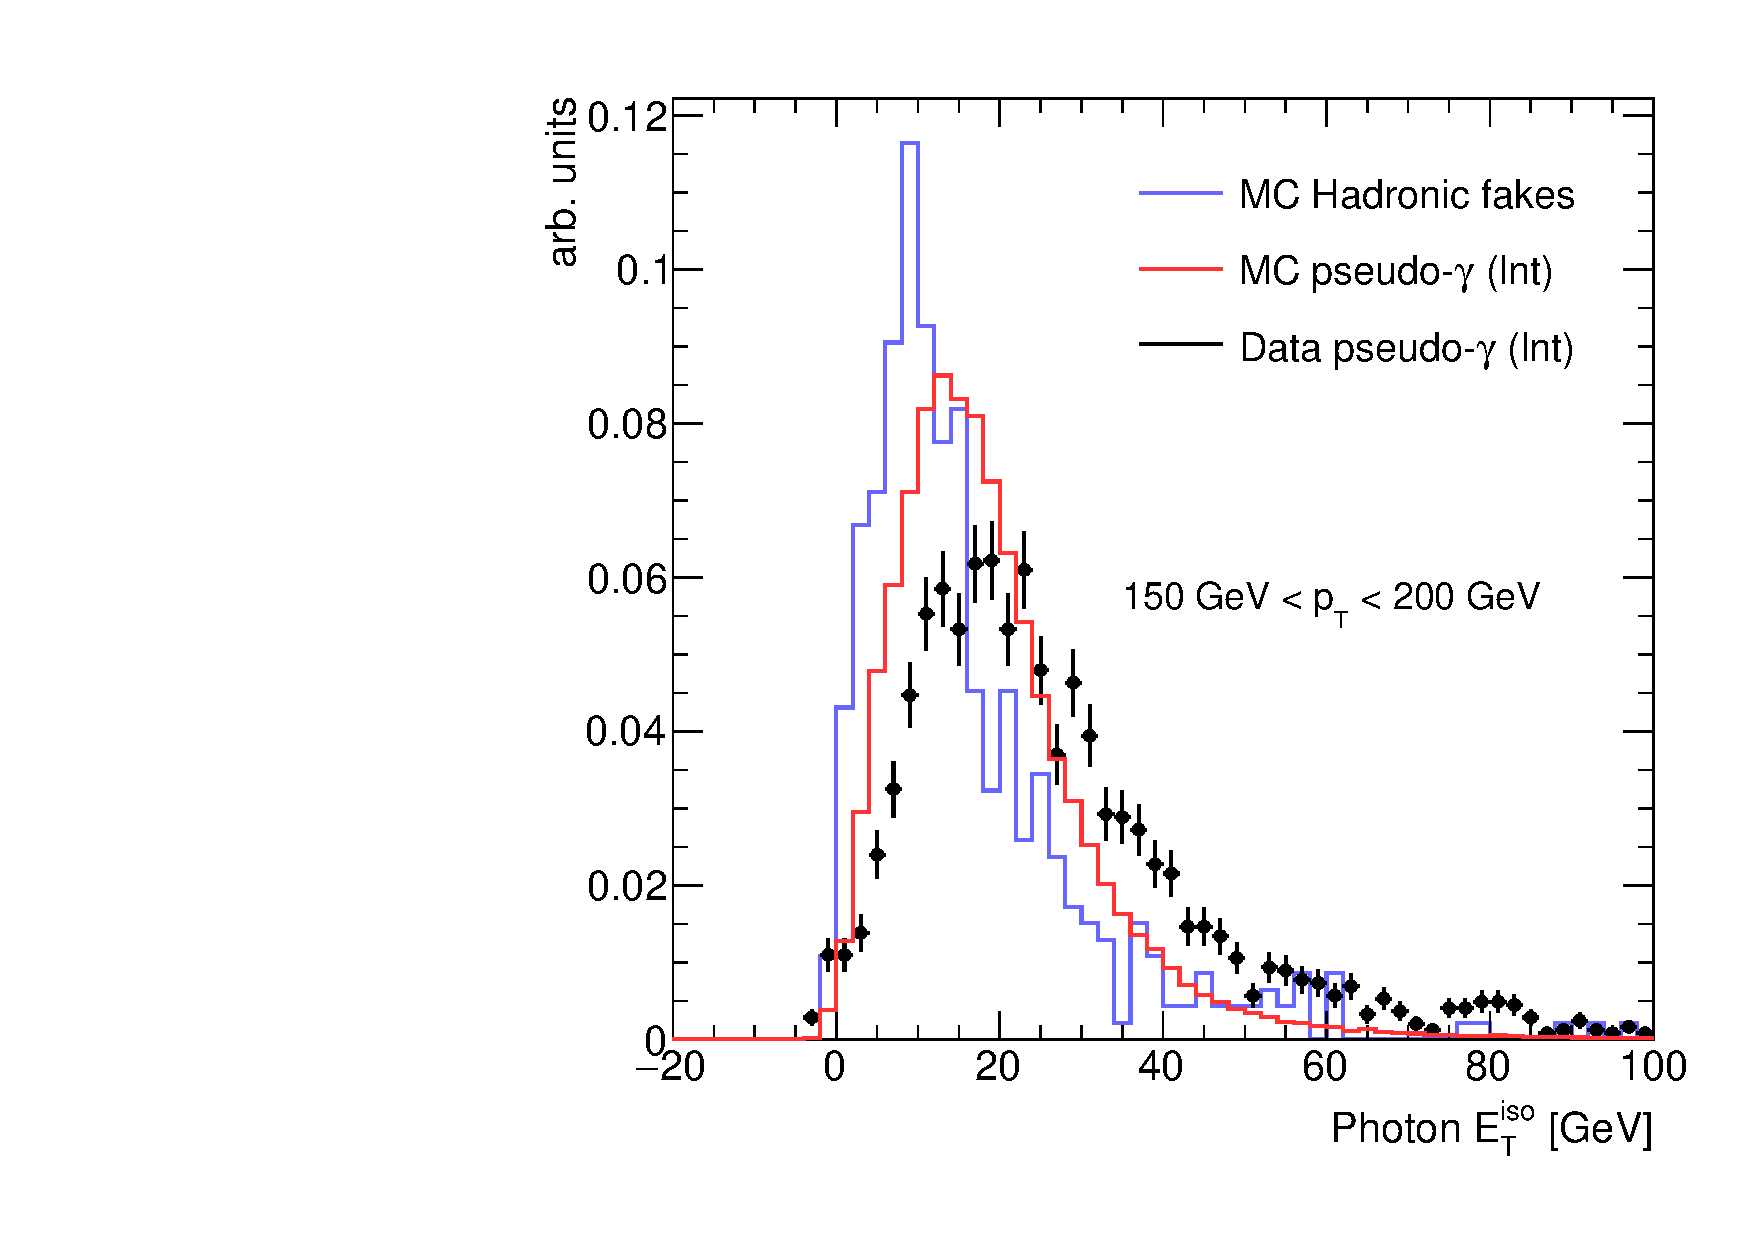
\includegraphics[width=0.49\textwidth]{figures/bkg_mc_pseudo_data_SR_l_ptbin}
  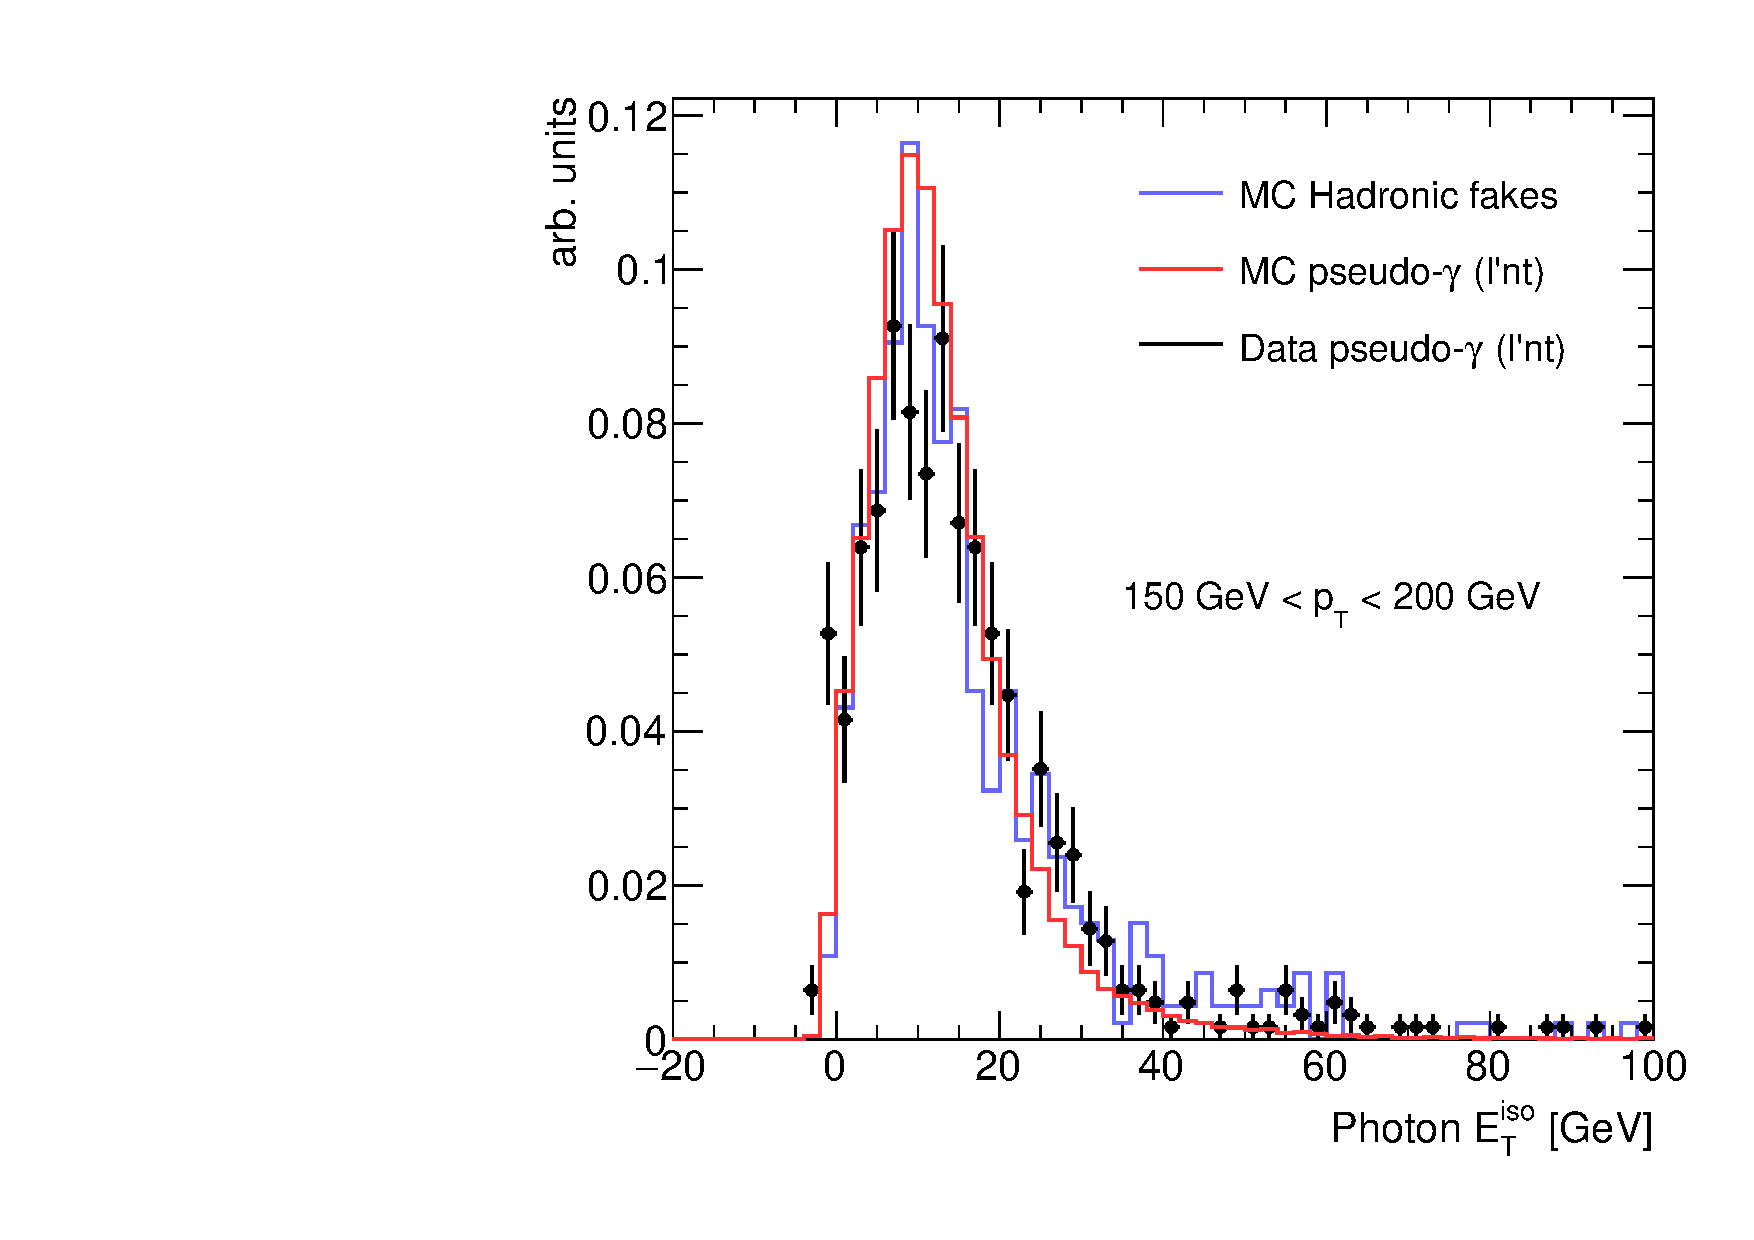
\includegraphics[width=0.49\textwidth]{figures/bkg_mc_pseudo_data_SR_lp_ptbin}

  \caption{Distribución de la energía de aislamiento para fotones falsos
    provenientes de decaimientos hadronicos (a nivel generador), comparada con
    la de pseudo-fotones obtenidos ....}
     %% Isolation distribution for truth MC photon fakes from hadronic decays, compared to pseudo-photon
    %% sample obtained in MC for background, obtained in the (right) nominal and (left) loose signal regions.}
  \label{fig:jetfake_mc_data}

\end{figure}

Mas aún, como se ve en la \cref{fig:jetfake_pseudo_data_pt}, los fotones L'NT
reproducen mejor el espectro de {\pt} de los fotones \emph{tight}, y no hace falta aplicar
una correcion por el {\pt}. Similarmente,
\cref{fig:jetfake_pseudo_data_BE} muestra la unica pequeña diferencia en la
región barrel y endcap.

%% Particularly for fake events, the extrapolation from the region used to derive the faking probability ratio and
%% the respective signal region might suffer from different topology and kinematics of the events in each case.
%% For this reason, the control region selection to derive the templates is kept close to the SR, as listed in {\tab} \ref{tab:cr_jetfake}.
%% An orthogonality requirement is placed on \MET ($50-150\gev$) and some SR cuts are loosened to retain statistics.
%% As expected, however, the larger the jet activity around the harder the photon isolation in the event. So the
%% \HT\ requirements can not be loosened much. This can be clearly observed in {\fig} \ref{fig:jetfake_pseudo_data_LR_VR},
%% for a loose (CRFJL: $>200 \gev$) and tight (CRFJ: $>600 \gev$) \HT\ selection. The latter is therefore used to
%% perform the combined fit and to compute the jet fake factor, as discussed in the next section.

\begin{table}[!htbp]
  \centering

  \caption{Definición de las regiones de control utilizadas para la estimación de los jets mal identificados como fotones.}
  \label{tab:cr_jetfake}

  %%$f_{j\to\gamma}$ fake factor derived in the CRFJ region. The numeric suffix indicates (when present) the SR associated to each region (SR2 or SR3).}
  \begin{tabular}{rcc}
    \hline
                                             &          CRFJ &       CRFJL \\
    \hline
    $\pt(\text{pseudo}-\gamma_1)$ [\gev] $>$ &           125 &         125 \\
    $\nleptons$                              &             0 &           0 \\
    \met [\gev]                              &   $[50, 150]$ & $[50, 150]$ \\
    $\njets \ge$                             &             2 &           2 \\
    $\pt^{j_1,j_2}$  [\gev]  $>$             &           100 &         100 \\
    $\dphijm >$                              &           0.4 &         0.4 \\
    \HT [\gev] $>$                           &           600 &         200 \\
    \hline
  \end{tabular}

\end{table}


\begin{figure}[!htbp]
  \centering

  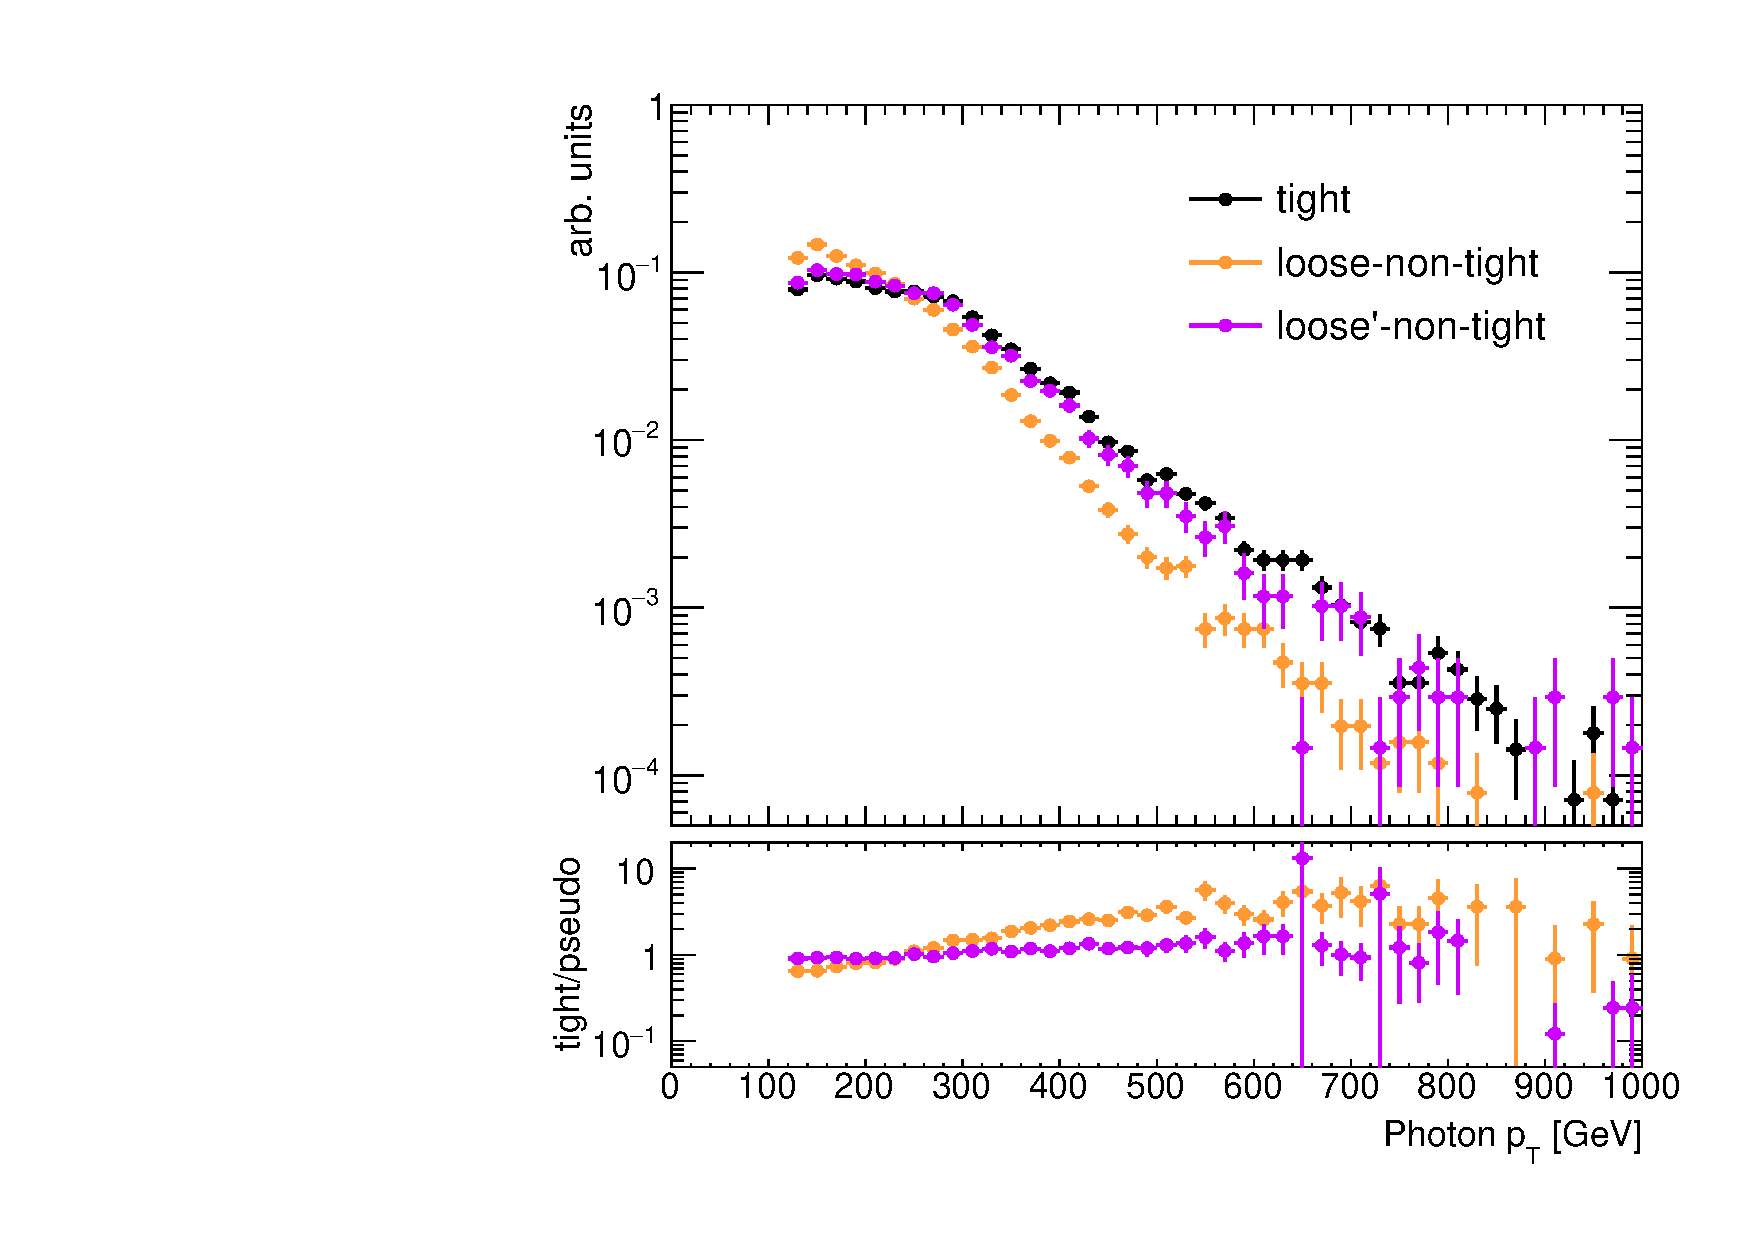
\includegraphics[width=0.49\textwidth]{figures/bkg_data_pseudo_tight_data_VR}

  \caption{Distribución del {\pt} del fotón para candidatos
    \emph{tight} y pseudo-fotones, luego de la selección  CRFJ.}
  \label{fig:jetfake_pseudo_data_pt}

\end{figure}

\begin{figure}[!htbp]
  \centering

  \includegraphics[width=0.49\textwidth]{figures/bkg_pseudo_data_SREB_l}
  \includegraphics[width=0.49\textwidth]{figures/bkg_pseudo_data_SREB_lp}

  \caption{Distribucion de la energia de aislamiento para pseudo-fotones loose-non-tight (izquierda) y loose'-non-tight (derecha),
    luego de la seleccion CRFJ, en la regiones de \emph{barrel} y \emph{endcap}.}
  \label{fig:jetfake_pseudo_data_BE}

\end{figure}

\begin{figure}[!htbp]
  \centering

  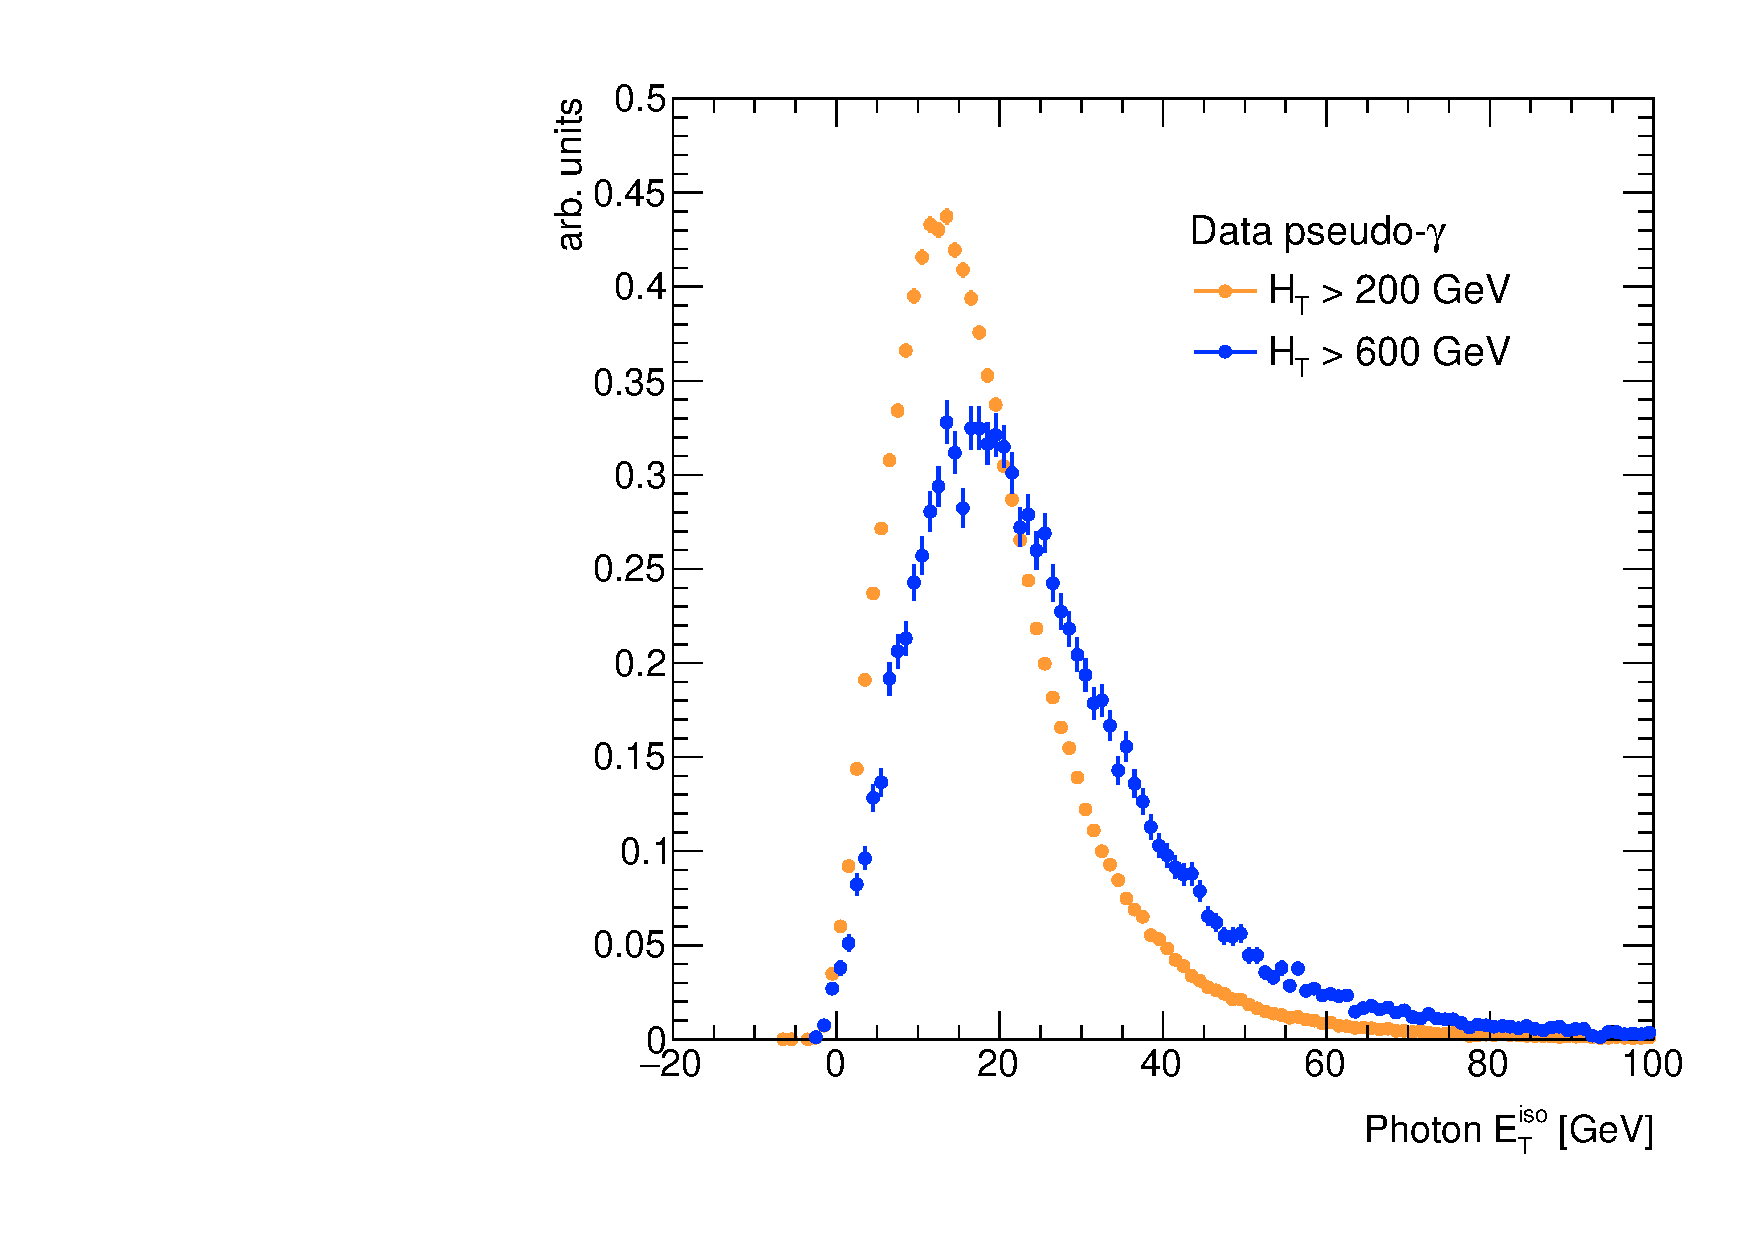
\includegraphics[width=0.49\textwidth]{figures/bkg_pseudo_data_SR_VR_l}
  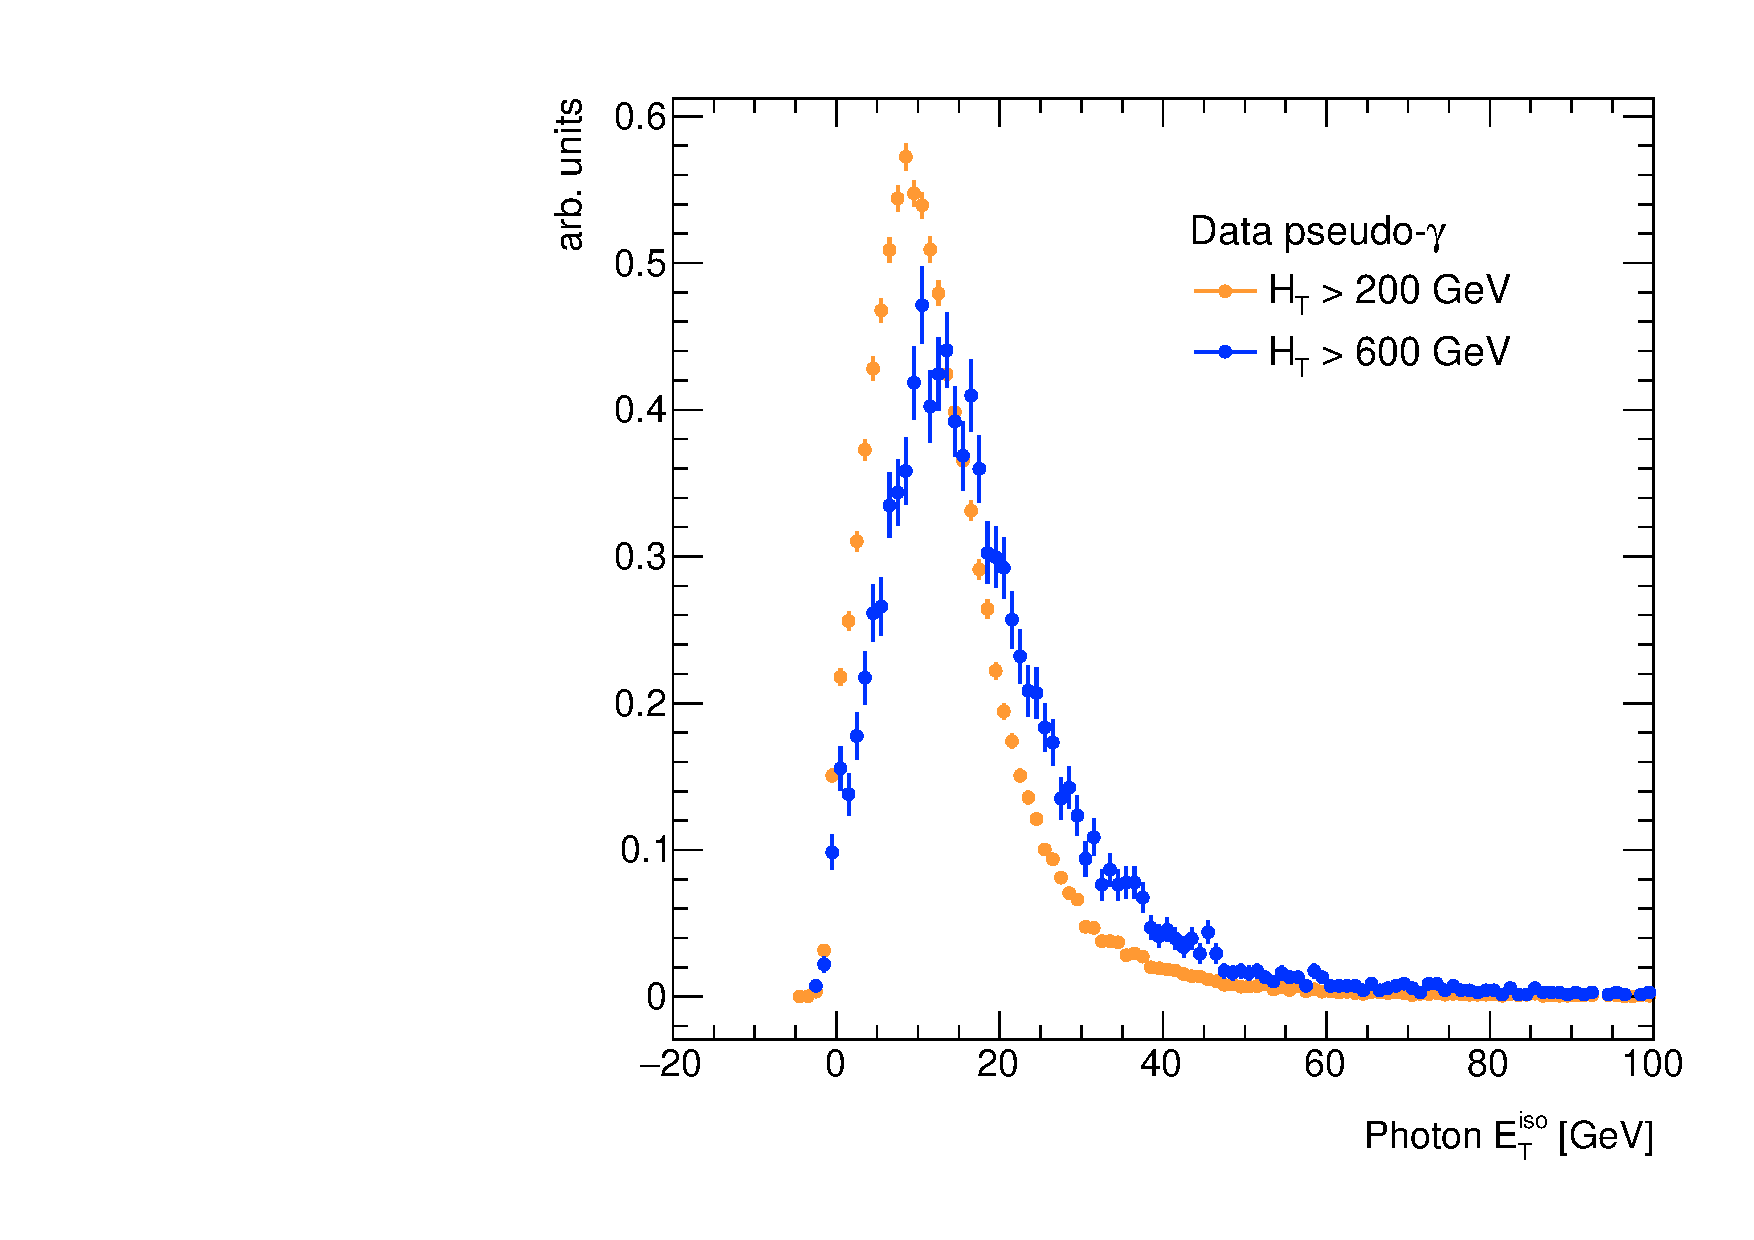
\includegraphics[width=0.49\textwidth]{figures/bkg_pseudo_data_SR_VR_lp}

  \caption{Distribucion de la energia de aislamiento para pseudo-fotones loose-non-tight (izquierda) y loose'-non-tight (derecha),
    luego de la seleccion con un corte en {\HT} CRFJL ($>200 \gev$) y CRFJ ($>600 \gev$).}
  \label{fig:jetfake_pseudo_data_LR_VR}

\end{figure}

Finalmente, se encuentra que la distribucion de los psuedp-fotones esta bien descripta en la region CRFJ port una funcion
Crystall-Ball. La distribucion en datos y el ajuste puede verse en la \cref{fig:jetfake_sigbkg}.
%% The parametrized template is used in the combined
%% fit to tight photon data to derive the jet fake rate.

%% \begin{figure}[h]
%%   \begin{center}
%%   \includegraphics[width=0.49\textwidth]{iso_fit_bkg_wpars}
%%   \caption{Fit to the observed isolation template for  loose'-non-tight pseudo-photon data in the VR.}
%%   \end{center}
%%   \label{fig:jetfake_bkg_template_fit}
%% \end{figure}

\subsection{Ajuste combinado y estimación del fondo} \label{sec:jet_fake_results}

%% A template fit to both signal and background distributions is then used to model the shape of the photon isolation
%% for each contribution, as shown in \cref{fig:jetfake_sigbkg}, together with the fitted parameters.
%The corresponding $\chi^2$/dof are 2.4 and 8.8 for signal and background templates with 240 points.
Se utiliza el modelo de señal y fondo descriptos en las secciones anteriores para
modelar la forma de la energía de aislamiento de los fotones, como se puede
apreciar en la \cref{fig:jetfake_sigbkg}.

La distribución de {\etiso} para todos los eventos que pasan los criterios de
selección de la región relajada (CRFJ) es ajustada a una combinación lineal de
los modelos de señal y fondo. El ajuste combinado y cada componente de la
distribución pueden verse en \cref{fig:jetfake_combfit}. Los parámetros son
inicializados con los valores extraídos de los ajustes individuales a la señal y
el fondo, y se los permite variar dentro de su incerteza
%As this fit is the source of the biggest systematic uncertainty the range of the parameters is then extend to two times the
%individual fit uncertainties to compute the systematic of the method.

Para estimar la incerteza sistemática, el ajuste combinado es realizado
sin ningún constrarin en los parámetros. La incerteza obtenida es del
50\% del valor de $f_{j\to\gamma}$, lo suficientemente grande para contener
cualquier potencial mismodelado de los templates.

%The fitted parameters for the signal, background and combined fits are tabulated in \Tab \ref{tab:jetfake_fit_pars}.
%% Los parametros estimados del ajuste combinado estan tabulados en la
%% \cref{tab:jetfake_fit_pars}.

El número de fotones total (N$_\text{tot}^\text{iso}$) y falsos
(N$_{j\to\gamma}^\text{iso}$) esperados en la región de control es obtenido
integrando las componentes de fondo y total del ajuste combinado sobre todo el
rango $\etiso<5\gev$, respectivamente:

\begin{itemize}
\item[] N$_{j\to\gamma}= 24143 \pm 56$

\item[] N$_\text{tot}= 281812 \pm 533$
\end{itemize}

La fracción $f_{j\to \gamma}$ es obtenida simplemente como el cociente
en la \cref{eq:jfake_formula}:

\begin{itemize}
\item[] $f_{j\to\gamma} = 0.0857 \pm 0.0002 \stat \pm 0.04 \;\syst$
\end{itemize}

\begin{figure}[!htbp]
  \centering

  \includegraphics[width=0.49\textwidth]{figures/iso_fit_sig_wpars}  \hfill
  \includegraphics[width=0.49\textwidth]{figures/iso_fit_bkg_wpars}

  \caption{Ajuste a las distribuciones de {\etiso} de señal
    (izquierda) y fondo (derecha) (right) en la región
    de control CRFJ.}
  \label{fig:jetfake_sigbkg}

\end{figure}

\begin{figure}[!htbp]
  \centering

  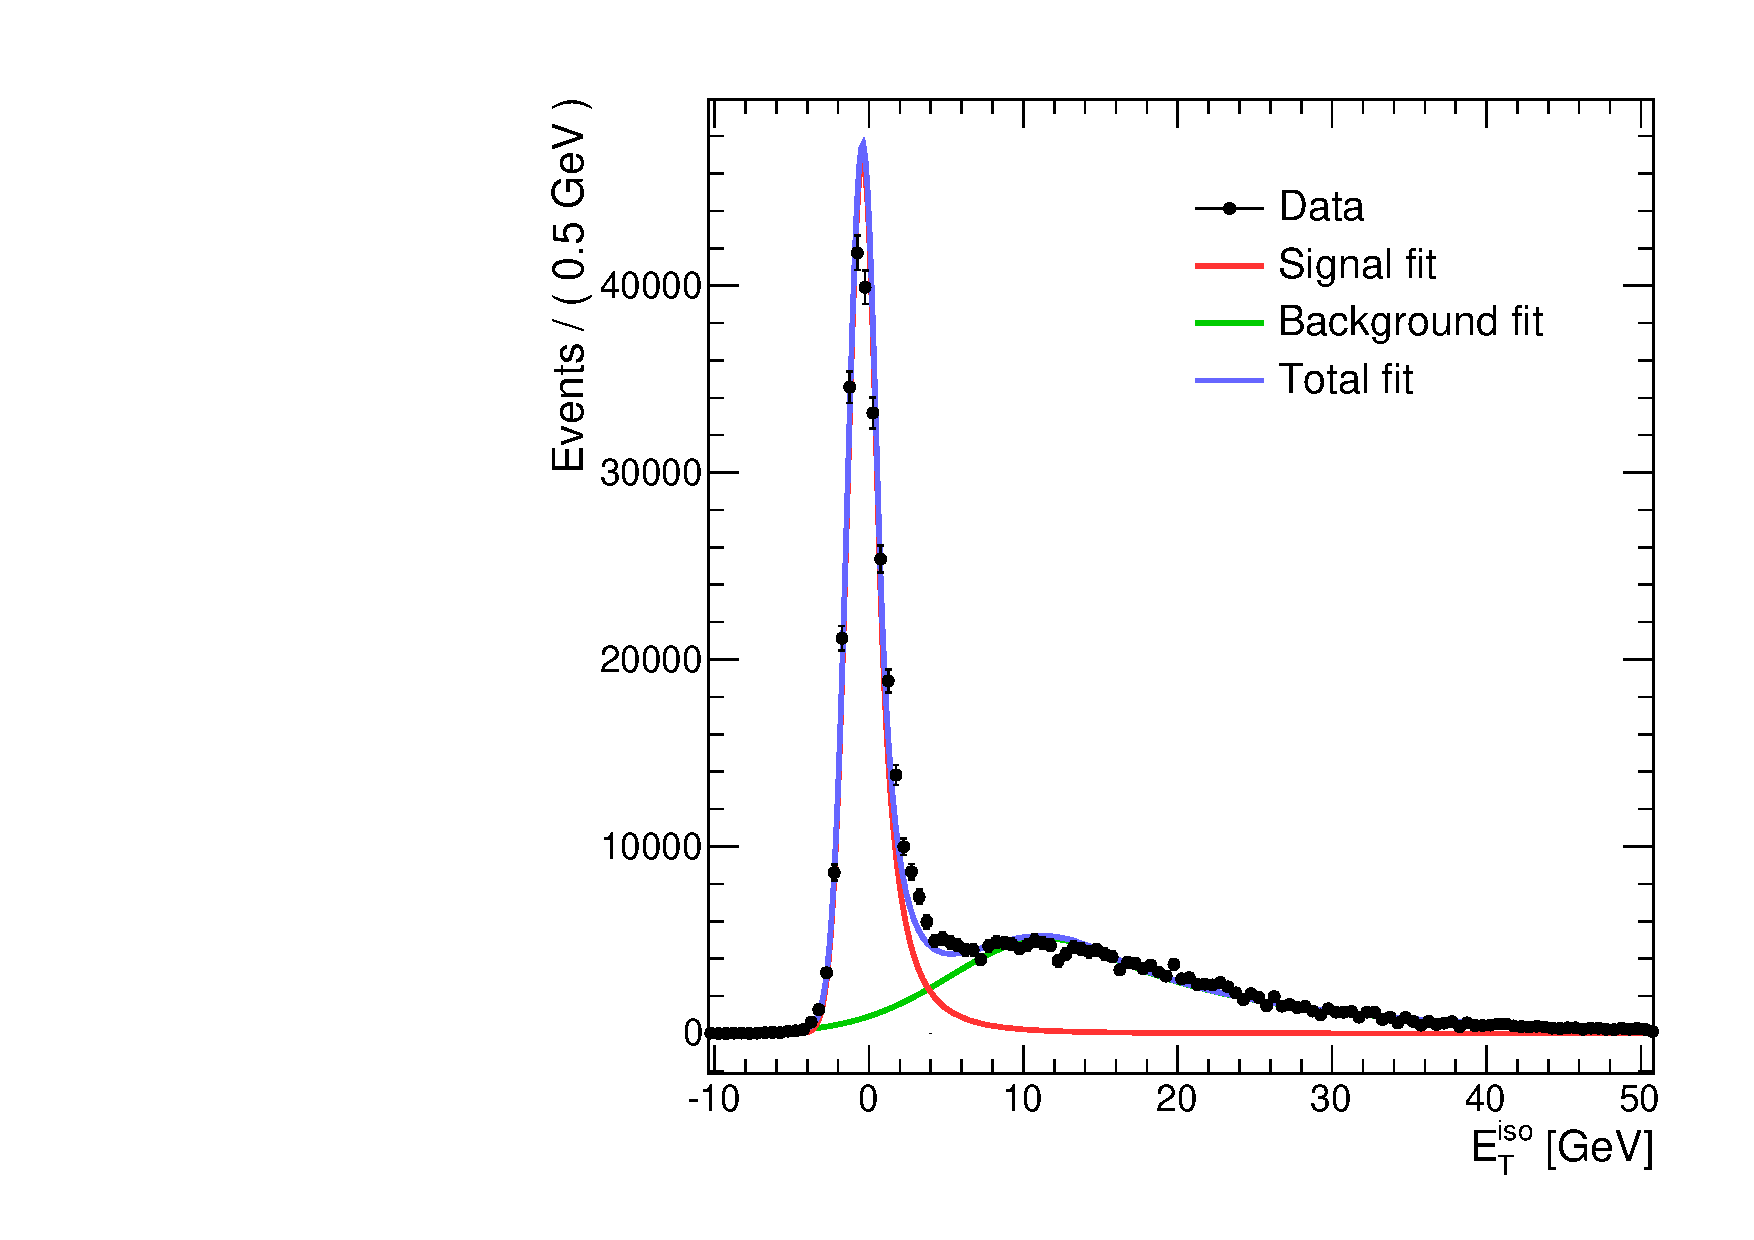
\includegraphics[width=0.49\textwidth]{figures/iso_fit_sarange}

  \caption{Ajuste combinado a la distribución de {\etiso}
    para los pseudo-fotones que pasan la selección de la región
    de control CRFJ (ver texto para detalles).}
  \label{fig:jetfake_combfit}

\end{figure}

%% \begin{table}[h!]
%%   \centering
%%   \caption{Fit parameters results from the combined fit to the isolation distribution of pseudo-photon data in CRFJ. Both signal and background were found to be well described by a Crystall Ball function.}
%%   \begin{tabular}{l l}
%%      Parameter &  Fit result \\
%%      \hline
%%      \verb|bkg_cb_alpha| & $-0.5932 \pm 0.0003$ \\
%%      \verb|bkg_cb_mean|  & $11.4897 \pm 0.0009 \GeV$ \\
%%      \verb|bkg_cb_n|     & $9.33 \pm 0.03$ \\
%%      \verb|bkg_cb_sigma| & $6.2862 \pm 0.0008 \GeV$ \\
%%      \verb|bkg_yield|    & $216579 \pm 500$ \\
%%      \hline
%%      \verb|sig_cb_alpha| & $-1.0460 \pm 0.0001$ \\
%%      \verb|sig_cb_mean|  & $-0.4175 \pm 0.003 \GeV$ \\
%%      \verb|sig_cb_n|     & $3.6675 \pm 0.0007$ \\
%%      \verb|sig_cb_sigma| & $0.9819 \pm 0.0001$ \\
%%      \verb|sig_yield|    & $2654337 \pm 546$ \\
%%      \hline
%%    \end{tabular}
%%     \label{tab:jetfake_fit_pars}
%% \end{table}

El número de jets identificados erróneamente como fotones puede ser estimado
utilizando la fracción $f_{j\to\gam}$ como,

\begin{equation}\label{eq:njfakes}
  N_{j\to\gam} = f_{j\to\gam} \cdot N_\mathrm{tight}
\end{equation}

Para estimar la contribucion en las SR, sin necesidad de utilizar el numero
de eventos en las SR, para poder estimar el número de jets
mal identificados como fotones en las SR, se parametrizó este número como
función de \met, como se puede ver en \cref{fig:jetfake_nfakes_met}, utilizando
una función exponencial $N_{j\to\gam} = \exp(a+b \, \met)$. Los valores de
$a$ y $b$ obtenidos del ajuste se muestran en la \cref{tab:exppars}.

\begin{table}[!htbp]
  \centering
  \caption{Parámetros que resultan del ajuste a la distribución de $N_{j\to\gam}$ como función de {\met} con una función exponencial $\exp(a+b\, \met)$.}
  \begin{tabular}{crr}
    \hline
    Parámetro &  {\SRL} & {\SRH} \\
     \hline
     a & $3.87 \pm 1.25$  &  $1.80 \pm 0.98$ \\
     b &  $-0.054 \pm 0.018$  & $-0.047 \pm 0,014$ \\
     \hline
  \end{tabular}
  \label{tab:exppars}
\end{table}


La contaminación esperada de jets falsos en las SR se estima integrando la
parametrización de $N_{j\to\gam}$ sobre la región de {\met} de cada SR.

\begin{align}
  N_{j\to\gam}^\text{\SRL} &= \int_{200}^{\infty} N_\text{fakes}(\met) \, d\met = 0.01 \pm 0.02 \\
  N_{j\to\gam}^\text{\SRH} &= \int_{300}^{\infty} N_\text{fakes}(\met) \, d\met = 0.0001 \pm 0.0001
\end{align}


\begin{figure}[!htbp]
  \centering
  \includegraphics[width=0.49\textwidth]{figures/nfakes_SR2}  \hfill
  \includegraphics[width=0.49\textwidth]{figures/nfakes_SR3}
  \caption{Parametrización del número de jets mal identificados como
    función de {\met}.\hl{Update plot}}
  \label{fig:jetfake_nfakes_met}
\end{figure}

El fondo de jets identificados como fotones es estimado similarmente en las
regiones de control y validación,
multiplicando el número de eventos observado en cada cosa por el factor
$f_{j\to\gamma}$.


%% The final background contamination expected from jets faking photons is obtained by weighting the number of events observed in data,
%% after the otherwise full tight SR selections detailed in sec \ref{sec:signal_regions} (i.e. only the photon identification requirement is reversed).


%% Indeed, no pseudo-photon event was ultimately observed after all CRJ selections. This leads to a
%% j$\to\gamma$ background estimate of $<0.07$ events. Consistently, MC studies have shown this
%% background to be small in the high \MET\ and \HT\ regimes on the final SRs. As seen in \Tab \ref{tab:mc_events_sr_phtype}, the
%% MC predicts a jet fake contamination of $0.10\pm 0.04$ and $0.02 \pm 0.02$ event for SR2 and SR3, respectively.
%% This supports the findings in the data, agreeing within the uncertainties. The final jet fake background yield is estimated as $N^\text{SR}_\text{jfakes} = 0.0^{+0.1}_{-0.0}$, which accommodates an extra $+0.03$ uncertainty from the comparison of the MC-data predictions.

%\tosolve{add check with MET-stepped predictions?}.


%In absence of observed events surviving the SR selection, a conservative estimate is computed under the assumption
%of one event in the pseudo photon sample for each signal region. It translates to a final yield of


%The final background contamination expected from jets faking photons was obtained by weighting the number of pseudo-photon events observed
%in data, after the otherwise full tight SR selections detailed in sec \ref{sec:signal_regions}. i.e. only the photon identification requirement is reversed.
%The results are summarized in \Tab \ref{tab:jetfake_yields}.
%
%\begin{table}[h!]
%  \centering
%  \caption{Number of misidentified jet events expected in the different signal regions. The unscaled number of pseudo-photons
%    is weighted by the $f/p$ ratio to get the final background yield from jet fakes in the three
%    analysis regions.}
%
%  \begin{tabular}{ccc}
%    \hline
%    \hline
%    Signal region & Unscaled & Weighted  \\
%    \hline
%%    SR1 & $4$ & $7.50$ \\
%    SR2 & $0$ & $0.00$ \\
%    SR3 & $0$ & $0.00$ \\
%    \hline
%    \hline
%  \end{tabular}
%  \label{tab:jetfake_yields}
%\end{table}


%% Two control samples are defined from the data to estimate the contamination in the SR of background events by electron or jet fake.
%% %The are the control samples used as inputs for the weighting procedure.
%% In the CSE sample the role of the photon is replaced by a \texttt{medium++} isolated electron and then weighted to get the final estimate
%% in the SR as described in sec \ref{sec:ewbackground}. Similarly, the jet$\to$photon background is obtained by weighting a pseudo-photon
%% sample (CSJ) defined from the SR selection by reversing the ID cuts satisfied by the high-\pt\ photon as explained in sec \ref{sec:jetfakes}.
%% To ensure orthogonality to the signal region, no tight-isolated photon is allowed in the CSJ selection above the SR {\pt} threshold. All selection
%% cuts are summarized in {\tab} \ref{tab:CRdd}.

%\tosolve{add table for CSE/CSJ definitions?}
%Regions CRE and CRJ are used to select a control sample for the electron and jet fakes data-driven methods. They are not constrained by the global likelihood fit used for the final background estimation.

%% \begin{table}[h!]
%%   \centering
%% \caption{Selection cuts for CSE and CSJ regions defined for the data-driven methods applied in this analysis, associated to each SR.}
%% \begin{tabular}{rcccc}
%%     \hline \hline
%%                                                &    CSE2 &     CSJ2 &    CSE3 &   CSJ3 \\
%%     \hline
%%     leading electron $\pt$ (\gev) $>$          &    125  &       -  &    300  &    300 \\
%%     leading pseudo-photon $\pt$ (\gev) $>$     &      -  &     125  &      -  &      - \\
%%     $\pt(\gamma_1)$ (\gev) (if any) $<$        &    125  &     125  &    125  &    125 \\
%%     N leptons                                  &      1  &       0  &      1  &      1 \\
%%     \met (\gev)                                & $>200$  &  $>200$  & $>300$  & $>300$ \\
%%     N jets $\ge$                               &      4  &       4  &      2  &      2 \\
%%     $\pt(j_2)$  (\gev)  $>$                    &    100  &     100  &     40  &     40 \\
%%     $\dphijm >$                                &    0.4  &     0.4  &    0.4  &    0.4 \\
%%     $\rt <$                                &   0.85  &    0.85  &      -  &      - \\
%%     $\dphijg <$                               &     -   &      -   &    2.0  &    2.0 \\
%%     \HT (\gev)                                 &     -   &      -   & $>800$  & $>800$ \\
%%     \hline \hline
%%   \end{tabular}
%% \label{tab:CRdd}
%% \end{table}
